\documentclass[12pt]{book}

%\usepackage{color}
\usepackage{xcolor}
\usepackage{listings}
\usepackage{array}
\usepackage{geometry}
\usepackage{graphicx}

\title{Discrete-Event Simulation\\
       of Queueing Systems in Java:\\
       The JSimulation and JQueues Libraries}
\author{Jan de Jongh}
\date{Release 5}

\lstset
{
  language=Java,
  basicstyle=\ttfamily,
  commentstyle=\textit,
  keywordstyle=\color{blue}\bfseries,
  tabsize=2,
  frame=single,
  escapeinside={<@}{@>}
}

\begin{document}

\maketitle

\chapter*{}

{\em This book is dedicated to Dick Epema, Graham Birtwistle, and Isi Mitrani.}

\tableofcontents

\chapter{Preface}

Queueing systems deal with the general notion of {\em waiting\ }
  for (the completion of) something.
They are ubiquitously and often annoyingly present in our everyday lives.
If there is anything we do most,
  it is probably {\em waiting\ } for something to
  happen (finally winning a non-trivial prize in the State Lottery
          after paying monthly tickets over the past thirty years),
  arrive (the breath-taking dress we ordered from that webshop
          against warnings in the seller's reputation blog),
  change (the reception of many severely bad hands in the poker game
          we just happened to ran into),
  stop (the constant flipping into red of traffic lights
        while we are just within breaking distance
        in our urban environment),
  or resume (the heater that regularly happens to have
             a mind of its own during
             winter months).

{\bf XXX}

\chapter{Introduction}

\chapter{Guided Tour}

\section{Getting Started}

\section{Creating and Running Queueing-System Simulations}

\subsubsection{A Simple Simulation with a First-Come First-Served Queue}

In order to perform a simulation study in \lstinline|jqueues|,
  the following four actions need to be taken:
\begin{itemize}
\item The creation of an event list;
\item The creation of one or more queues, and their attachment to the event list;
\item The selection of the method for listening to the queue(s), and/or the event list;
\item The creation of a workload consisting of jobs;
\item Running the event list.
\end{itemize}
Without much further ado, here's an example:

\begin{lstlisting}[
  caption={A simple simulation with a single FCFS\_B queue and ten jobs.},
  label=simExample1_main,
  basicstyle=\tiny]

    final SimEventList el = new DefaultSimEventList ();
    final int bufferSize = 2;
    final FCFS_B queue = new FCFS_B (el, bufferSize);
    queue.registerStdOutSimQueueListener ();
    for (int j = 0; j < 10; j++)
    {
      final double jobServiceTime = (double) 2.2 * j;
      final double jobArrivalTime = (double) j;
      final String jobName = Integer.toString (j);
      final SimJob job = new DefaultSimJob (null, jobName, jobServiceTime);
      SimEntityEventScheduler.scheduleJobArrival (job, queue, jobArrivalTime);
    }
    el.run ();

\end{lstlisting}

In Listing \ref{simExample1_main},
  we first create a single event list of type \lstinline|DefaultSimEventList|
  and a \lstinline|FCFS_B| queue.
On the queue, we invoke its default "listener",
  issuing notification to the standard output.
Subsequently,
  we create ten jobs named "0", "1", "2", $\ldots$,
  scheduled for arrival at the queue
  at $t=0$, $t=1$, $t=2$, $\ldots$,
  respectively.
Finally, we "run" the event list, i.e.,
  let it process the arrivals.

The event list type
  \lstinline|DefaultSimEventList|
  will suffice for almost all practical cases,
  but it is essential to note already that
  a {\em single\/} event-list instance is typically used
  throughout {\em any\/} simulation program.
Its purpose of the event list is to hold scheduled {\em events\/}
  in non-decreasing order of {\em schedule time},
  and, upon request (in this case through \lstinline|el.run|),
  starts processing the scheduled events in sequence,
  invoking their associated {\em actions}.
In this case,
  the use of events remains hidden,
  because jobs are scheduled through the use of utility method
  \lstinline|scheduleJobArrival|.

The queue of choice is the First-Come First-Served queue
  with limited buffer size, \lstinline|FCFS_B|,
  described in more detail in Section \ref{FCFS_B}.
The constructor takes two arguments,
  the event list \lstinline|el|
  and the buffer size.
The queueing system consists of a queue with only \lstinline|B|
  places to hold jobs,
  and a single server that "serves" the jobs in the queue in order
  of their arrival.
If a job arrives at the \lstinline|FCFS_B| system
  while all places in the queue are occupied by other jobs,
  the arriving job is denied access to the system,
  and is {\em dropped}.
Once a queue has finished serving the (single) job,
  the job {\em departs\/} from the system.

So how long does it take to serve a job?
Well, in \lstinline|jqueues|,
  the default behavior is that
  a queue requests the job for its
  {\em required service time},
  and we set a fixed service time (at {\em any\/} queue)
  for each job upon creation as the third argument of the constructur.
The first argument of the \lstinline-DefaultSimJob-
  is the event list to which it is to be attached.
For jobs (well, at least the ones derived from \lstinline|DefaultSimJob|),
  it is often safe to set this to \lstinline|null|,
  although we could have equally well set it to \lstinline|el|.
However, queues must always be attached to the event list;
  a \lstinline|null| value upon construction will throw an exception.

The (approximate) output of the code fragment of Listing \ref{simExample1_main}
is shown in Listing \ref{simExample1_out} below.

\begin{lstlisting}[
  caption={Example output of Listing \ref{simExample1_main}.},
  label=simExample1_out,
  basicstyle=\tiny]

StdOutSimQueueListener t=0.0, entity=FCFS_B[2]: UPDATE.
StdOutSimQueueListener t=0.0, entity=FCFS_B[2]: STATE CHANGED:
  => ARRIVAL [Arr[0]@FCFS_B[2]]
  => START [Start[0]@FCFS_B[2]]
  => DEPARTURE [Dep[0]@FCFS_B[2]]
StdOutSimQueueListener t=0.0, queue=FCFS_B[2]: ARRIVAL of job 0.
StdOutSimQueueListener t=0.0, queue=FCFS_B[2]: START of job 0.
StdOutSimQueueListener t=0.0, queue=FCFS_B[2]: DEPARTURE of job 0.
StdOutSimQueueListener t=1.0, entity=FCFS_B[2]: UPDATE.
StdOutSimQueueListener t=1.0, entity=FCFS_B[2]: STATE CHANGED:
  => ARRIVAL [Arr[1]@FCFS_B[2]]
  => START [Start[1]@FCFS_B[2]]
  => STA_FALSE [StartArmed[false]@FCFS_B[2]]
StdOutSimQueueListener t=1.0, queue=FCFS_B[2]: ARRIVAL of job 1.
StdOutSimQueueListener t=1.0, queue=FCFS_B[2]: START of job 1.
StdOutSimQueueListener t=1.0, queue=FCFS_B[2]: START_ARMED -> false.
StdOutSimQueueListener t=2.0, entity=FCFS_B[2]: UPDATE.
StdOutSimQueueListener t=2.0, entity=FCFS_B[2]: STATE CHANGED:
  => ARRIVAL [Arr[2]@FCFS_B[2]]
StdOutSimQueueListener t=2.0, queue=FCFS_B[2]: ARRIVAL of job 2.
StdOutSimQueueListener t=3.0, entity=FCFS_B[2]: UPDATE.
StdOutSimQueueListener t=3.0, entity=FCFS_B[2]: STATE CHANGED:
  => ARRIVAL [Arr[3]@FCFS_B[2]]
StdOutSimQueueListener t=3.0, queue=FCFS_B[2]: ARRIVAL of job 3.
StdOutSimQueueListener t=3.2, entity=FCFS_B[2]: UPDATE.
StdOutSimQueueListener t=3.2, entity=FCFS_B[2]: STATE CHANGED:
  => DEPARTURE [Dep[1]@FCFS_B[2]]
  => START [Start[2]@FCFS_B[2]]
StdOutSimQueueListener t=3.2, queue=FCFS_B[2]: DEPARTURE of job 1.
StdOutSimQueueListener t=3.2, queue=FCFS_B[2]: START of job 2.
StdOutSimQueueListener t=4.0, entity=FCFS_B[2]: UPDATE.
StdOutSimQueueListener t=4.0, entity=FCFS_B[2]: STATE CHANGED:
  => ARRIVAL [Arr[4]@FCFS_B[2]]
StdOutSimQueueListener t=4.0, queue=FCFS_B[2]: ARRIVAL of job 4.
StdOutSimQueueListener t=5.0, entity=FCFS_B[2]: UPDATE.
StdOutSimQueueListener t=5.0, entity=FCFS_B[2]: STATE CHANGED:
  => ARRIVAL [Arr[5]@FCFS_B[2]]
  => DROP [Drop[5]@FCFS_B[2]]
StdOutSimQueueListener t=5.0, queue=FCFS_B[2]: ARRIVAL of job 5.
StdOutSimQueueListener t=5.0, queue=FCFS_B[2]: DROP of job 5.
StdOutSimQueueListener t=6.0, entity=FCFS_B[2]: UPDATE.
StdOutSimQueueListener t=6.0, entity=FCFS_B[2]: STATE CHANGED:
  => ARRIVAL [Arr[6]@FCFS_B[2]]
  => DROP [Drop[6]@FCFS_B[2]]
StdOutSimQueueListener t=6.0, queue=FCFS_B[2]: ARRIVAL of job 6.
StdOutSimQueueListener t=6.0, queue=FCFS_B[2]: DROP of job 6.
StdOutSimQueueListener t=7.0, entity=FCFS_B[2]: UPDATE.
StdOutSimQueueListener t=7.0, entity=FCFS_B[2]: STATE CHANGED:
  => ARRIVAL [Arr[7]@FCFS_B[2]]
  => DROP [Drop[7]@FCFS_B[2]]
StdOutSimQueueListener t=7.0, queue=FCFS_B[2]: ARRIVAL of job 7.
StdOutSimQueueListener t=7.0, queue=FCFS_B[2]: DROP of job 7.
StdOutSimQueueListener t=7.6000000000000005, entity=FCFS_B[2]: UPDATE.
StdOutSimQueueListener t=7.6000000000000005, entity=FCFS_B[2]: STATE CHANGED:
  => DEPARTURE [Dep[2]@FCFS_B[2]]
  => START [Start[3]@FCFS_B[2]]
StdOutSimQueueListener t=7.6000000000000005, queue=FCFS_B[2]: DEPARTURE of job 2.
StdOutSimQueueListener t=7.6000000000000005, queue=FCFS_B[2]: START of job 3.
StdOutSimQueueListener t=8.0, entity=FCFS_B[2]: UPDATE.
StdOutSimQueueListener t=8.0, entity=FCFS_B[2]: STATE CHANGED:
  => ARRIVAL [Arr[8]@FCFS_B[2]]
StdOutSimQueueListener t=8.0, queue=FCFS_B[2]: ARRIVAL of job 8.
StdOutSimQueueListener t=9.0, entity=FCFS_B[2]: UPDATE.
StdOutSimQueueListener t=9.0, entity=FCFS_B[2]: STATE CHANGED:
  => ARRIVAL [Arr[9]@FCFS_B[2]]
  => DROP [Drop[9]@FCFS_B[2]]
StdOutSimQueueListener t=9.0, queue=FCFS_B[2]: ARRIVAL of job 9.
StdOutSimQueueListener t=9.0, queue=FCFS_B[2]: DROP of job 9.
StdOutSimQueueListener t=14.200000000000001, entity=FCFS_B[2]: UPDATE.
StdOutSimQueueListener t=14.200000000000001, entity=FCFS_B[2]: STATE CHANGED:
  => DEPARTURE [Dep[3]@FCFS_B[2]]
  => START [Start[4]@FCFS_B[2]]
StdOutSimQueueListener t=14.200000000000001, queue=FCFS_B[2]: DEPARTURE of job 3.
StdOutSimQueueListener t=14.200000000000001, queue=FCFS_B[2]: START of job 4.
StdOutSimQueueListener t=23.0, entity=FCFS_B[2]: UPDATE.
StdOutSimQueueListener t=23.0, entity=FCFS_B[2]: STATE CHANGED:
  => DEPARTURE [Dep[4]@FCFS_B[2]]
  => START [Start[8]@FCFS_B[2]]
StdOutSimQueueListener t=23.0, queue=FCFS_B[2]: DEPARTURE of job 4.
StdOutSimQueueListener t=23.0, queue=FCFS_B[2]: START of job 8.
StdOutSimQueueListener t=40.6, entity=FCFS_B[2]: UPDATE.
StdOutSimQueueListener t=40.6, entity=FCFS_B[2]: STATE CHANGED:
  => DEPARTURE [Dep[8]@FCFS_B[2]]
  => STA_TRUE [StartArmed[true]@FCFS_B[2]]
StdOutSimQueueListener t=40.6, queue=FCFS_B[2]: DEPARTURE of job 8.
StdOutSimQueueListener t=40.6, queue=FCFS_B[2]: START_ARMED -> true.

\end{lstlisting}

Apart from the \lstinline-STATE CHANGED-, \lstinline-UPDATE-
  and \lstinline-START_ARMED- lines in the output,
  the notifications pretty much speak for themselves.
We even get notified when jobs start service (\lstinline-START-),
  and when they are dropped (jobs $5$, $6$, and $7$)
  by the queue (\lstinline -DROP-).
The \lstinline-START_ARMED- notifications
  refer to state changes in a special boolean attribute of a
  queue named its \lstinline-StartArmed- property.
It is explained in detail in Section \ref{sec-start-armed}
  but since you will hardly need it in practical applications,
  we will not delve into it.
Suffice it to say that \lstinline|StartArmed| property
  reveals in some strange way
  whether the queue {\em would\/}
  start a hypothetical arriving job
  if several additional conditions are also met.
It is crucial for the implementation
  of more complex queueing systems.

The remaining two notification types, \lstinline|UPDATE| and \lstinline|STATE CHANGED|
  are essential, however, and require special attention.
We will however, defer their discussion for now.

\subsubsection{Creating and Registering Listeners}

\subsubsection{The \lstinline|UPDATE| and \lstinline|STATE CHANGED| Notifications}

As you may have spotted,
  events are actually reported twice,
  once as part of a \lstinline|STATE CHANGED| notification,
  followed by a separate notification specific to the event type
  (\lstinline-ARRIVAL-, \lstinline-DEPARTURE-, etc.).
As a matter of fact, these separate notifications are merely a courtesy
  of the queue as it is only required to issue
  \lstinline|UPDATE|, \lstinline|STATE CHANGED| and \lstinline|RESET| notifications.

In order to understand this,
  we must realize that in {\em any\/} discrete-event simulation,
  the entities (like queues) involved possess an individual {\em state\/}
  that can only change at discrete moments in time (the {\em epochs\/}),
  and as a result of an {\em operation\/} on the entity at that time.
This is explained grapically in Figure \ref{fig:SimpleSimulationOverview}.

\begin{figure}[h]
\label{fig:SimpleSimulationOverview}
\caption{The relations between simulation time, epochs,
	 the event list, scheduled events, and actions,
	 as well their impact on notifications from
	 and operations on
	 (the state of) an entity.}
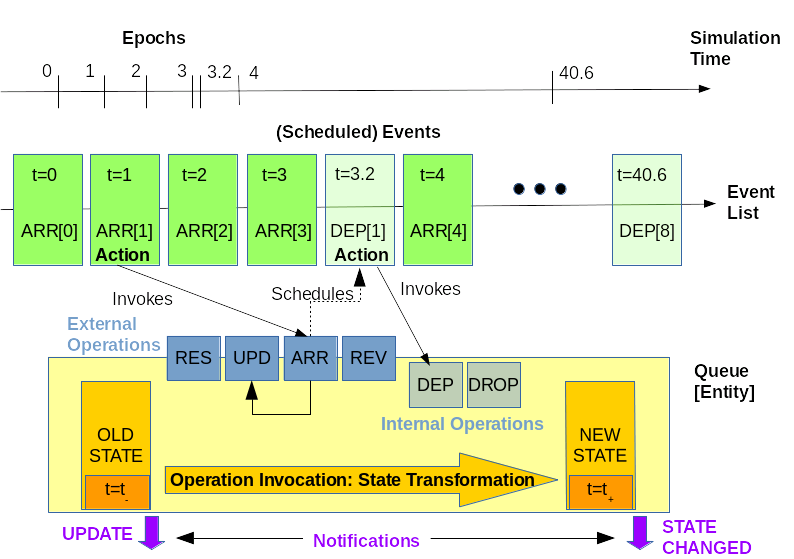
\includegraphics[width=\textwidth]{SimpleSimulationOverview}
\end{figure}

In the top of the figure,
  we show the simulation time and some of the epochs
  from the example.
During a simulation run, the simulation time increases monotonically
  as a function of "real time".
What this says is that the simulation time does not
  "strictly decrease" in real time,
  but at the same time,
  that's pretty much the only requirement
  on the relation between real time
  and simulation time.
For instance,
  processing the epochs between $t=0$ and $t=9$
  may take several minutes in real time,
  whereas epochs between $t=9$ and $t=100$
  could be done in a mere second\footnote{
This is not to say that is is impossible or even hard
  to let simulation time progress
  (roughly) at the same rate as real time,
  or at some scaled version of it.
However, in discrete-event simulation,
  the relationship between real time and simulation time
  is generally considered unimportant.}

Below the simulation-time line,
  we show the event list and some of the scheduled events
  from the example.
The apparent equal distance between the events
  is actually on pupose.
The event list is really not concerned with the
  simulation-time differences between adjacent events.
No matter how large the time interval between an
  event and its predecessor,
  in between (basicaly) nothing happened:
  There were not events,
  and hence,
  no state changes.
Going back to the figure,
  we scheduled the arrival events ourselves
  before processing the event list,
  but we also see two "departure events"
  we did not schedule.
In fact, these events were scheduled by the
  queue, in response to previous events.
For instance, when job $1$ arrives at $t=1$ (simulation time),
  it is taken into service immediately,
  and after requesting the service time from job $1$ ($2.2$),
  it schedules a {\em departure event\/} at $t=3.2$,
  shown in a somewhat different color because we
  did not schedule this ourselves (we are not even allowed to do so).
This shows an important aspect of the event list while processing it:
  in general, the actions taken while processing the event list have
  full freedom to schedule new events,
  as long as they are not in the past.
This, admittedly, is not clear from the figure.
What is essential to remember is that a scheduled event
  await its turn while the event list is being processed,
  and the event list invokes the event's action
  when it has processed all preceding events.

Assuming the event's action involves the queue in question,
  we now turn our attention to the bottom part of the figure,
  showing our queue from the example, the \lstinline|FCFS_B| queue.
We assume the arrival event at $t=1$ is processed by the event list,
  and the net effect of this (i.e., the action of the event)
  is the invokation of the arrival operation on the queue
  (with the job $1$ as its argument).
As a result of this operation,
  the state of the queue will transform,
  and registered listeners to the queue will be informed
  of the new state upon completion of the operation.
This, effectively, is the \lstinline|STATE CHANGED| notification.
In the figure this is shown with the right-pointing arrow at the bottom
  from \lstinline|OLD STATE| to \lstinline|NEW STATE|,
  and the \lstinline|STATE CHANGED| notification below that.

However, before doing anything,
  the arrival operation invokes
  the so-called \lstinline|UPDATE| operation,
  which exposes the {\em old\/} state
  to listeners and internally registered "hooks",
  and, subsequently, increases the most essential state
  property, the {\em last update time}.
By now, you should realize that
  as the event list progresses in simulation time,
  queues (or better, {\em entities\/})
  that are not affected by the events processed
  will not be bothered at all.
Yet a queue needs to assure that time-stamped operations
  never lie in the past,
  so they need to maintain a notion of simulation time themselves.
The importance of the \lstinline|UPDATE| notification
  lies in {\em statistics gathering},
  in which it is essential to know exactly
  during which (non-trivial) intervals
  the state of a queue did {\em not\/} change,
  and the lenght of such intervals.
As long as you are not involved in statistics-gathering,
  you can safely ignore these notifications,
  otherwise,
  you can find more details in Section \ref{sec:statistics}.

Once the \lstinline|UPDATE| operation has been
  fulfilled, the \lstinline|ARR| (job arrival) operation,
  in this particular case,
  checks the number of jobs waiting,
  and drops the arriving job if the number is $2$ ($=$\lstinline|B|)
  by invoking the internal operation \lstinline|DROP|.
However, for job $1$ in the example,
  it finds an empty waiting area,
  and, in addition, no job being served at the server.
This means that the job is taking into service immediately
  (the \lstinline|START| internal operation),
  and since the required service time is non-zero,
  the queue schedules a {\em departure event\/}
  at $t=3.2$.
The departur event, in turn,
  will invoke the internal \lstinline|DEP| (job departure)
  event because of which the job
  will eventually depart from the queueing system.

So, what more is there to say.
Well, we seem to have so called {\em external\/}
  and {\em internal\/} operations,
  the latter of which we cannot schedule ourselves
  (departures, drops, $\ldots$).
In a way, the external operations allow us
  to subject a queue to some kind of {\em workload\/}
  consisting of arriving jobs
  (as well as of, yet undescribed, other external operations on the queue).
The internal operations, on the other hand,
  are always involved from within the queue itself,
  either as a response to a scheduled event,
  or as a response to an invocation of an external operation
  in combination with a state condition
  (e.g., the arrival of a job while $2$ jobs are already waiting
  causes the internal \lstinline|DROP| operation to be invoked).
 
\begin{itemize}
	\item {\bf XXX}
	\item Atomicity of Operations and Notifications and their importance.
	\item Queue Invariants.
	\item \lstinline|RESET| operation.
	\item \lstinline|UPDATE| operations.
	\item When does a simulation end?
	\item Simultaneous events?
	\item Listeners and Listener Types.
	\item Remaining Operations (QAV, SAC, REV, AREV).
\end{itemize}

\chapter{Events, Event Lists and Actions}

This chapter describes the event and event-list features
  that are available from the \lstinline{jsimulation} package.
Note that \lstinline{jsimulation} is a dependency of \lstinline{jqueues}.

\section{Creating the Event List and Events}

At the very heart of every simulation experiment
  in \lstinline{jqueues}
  is the so-called {\em event list}.
The event list obviously holds the events,
  keeps them ordered,
  and maintains a notion of "where we are" in a simulation run.
Together, an event list and the events it contains define
  the precise sequence of actions taken in a simulation.
The following code snipplet shows how to create an event list and
  schedule two (empty) events, one at $t_{1}=5.0$ and one at $t_{2}=10$,
  and print the resulting event list on \lstinline{System.out}:
\begin{lstlisting}
final SimEventList el = new DefaultSimEventList ();
final SimEvent e1 = new DefaultSimEvent (5.0);
final SimEvent e2 = new DefaultSimEvent (10.0);
el.add (e1);
el.add (e2);
el.print ();
\end{lstlisting}
In \lstinline{jsimulation},
  the event list is of type \lstinline{SimEventList};
  events are of type \lstinline{SimEvent},
  respectively.
Since both of them are Java {\em interfaces}, you need implementing classes
  to instantiate them: \lstinline{DefaultSimEventList} for an event list;
  \lstinline{DefaulSimEvent} for an event.
Typically,
  you instantiate a single event list for a simulation experiment,
  and numerous events.

The \lstinline{double} argument in the \lstinline{DefaultSimEvent} constructor
  (of which there are several)
  is the {\em schedule time\/} of the event on the event list.
Perhaps surprisingly,
  in \lstinline{jsimulation},
  the schedule time is actually held on the event,
 {\em not\/} on the event list.
Also, a \lstinline{SimEventList} is inheriting from \lstinline{SortedSet}
  from the Java Collections Framework.
These choices have the following consequences:
\begin{itemize}
  \item Each \lstinline{SimEvent} can be present {\em at most once\/} in a \lstinline{SimEventList}.
        You cannot reuse a single event instance (like a job creation and arrival event)
          by scheduling it multiple times on the event list.
        Instead, you must either use separate event instances, or reschedule the event
          the moment it leaves the event list.
  \item You cannot (more precisely, {\em should not\/}) modify the time on the event while it is
          scheduled on an event list.
  \item You always have access to the (intended) schedule time of the event, without having to
          refer to an event list (if the event is scheduled at all) or use a separate
          variable to keep and maintain that time.
  \item The events must be equipped with a {\em total ordering\/} (imposed by \lstinline{SortedSet})
          and distinct events should not be equal (imposed by us).
          This means that for each pair of (distinct) events scheduled on a \lstinline{SimEventList},
          one of them is always strictly larger than the other
          (in the ordering, they cannot be "equal").
\end{itemize}

The output of the code snipplet is something like\footnote{
We may have improved the layout in the meantime.}:
\begin{lstlisting}[basicstyle=\tiny]
SimEventList {X}.DefaultSimEventList@{Y}, class=DefaultSimEventList, time=-Infinity:
  t=5.0, name=No Name, object=null, action=null.
  t=10.0, name=No Name, object=null, action=null.
\end{lstlisting}
The output shows the name of the event list (as obtained from its \lstinline{toString} method)
  and the current time ($-\infty$) in the first row, and then the events in the list
  in the proper order.
By the way, we modified the output; the markers \lstinline|{X}| and \lstinline|{Y}|
  represents strings that most likely deviate on your system.

The output also shows the four properties of an event: its time, name, user object, and action.
These will be described in more detail in the next section.

\section{Event Properties and Event Constructors}

A \lstinline{SimEvent} has the following properties:
\begin{itemize}
\item Time:   The (intended) schedule time of the event (default $-\infty$).
\item Name:   The name of the event, which is only used for logging and output (default "No Name").
\item Object: A general-purpose object available for storing information associated with the event
              (\lstinline{jsimulation} nor \lstinline{jqueues} uses this field; its
              default value is \lstinline{null}).
\item Action: The action to take, a \lstinline{SimEventAction} (default \lstinline{null}),
                described in the next section.
\end{itemize}
Each property has corresponding getter and setter methods:

\begin{tabular}{|l|}
  \hline
  {\bf Properties of \lstinline|SimEvent|} \\
  \hline
  \lstinline[basicstyle=\footnotesize]!double getTime ()! \\
  \lstinline[basicstyle=\footnotesize]!void setTime (double)! \\
  \hline
  \lstinline[basicstyle=\footnotesize]!String getName ()! \\
  \lstinline[basicstyle=\footnotesize]!void setName (String)! \\
  \hline
  \lstinline[basicstyle=\footnotesize]!T getObject ()! \\
  \lstinline[basicstyle=\footnotesize]!void setObject (T)! \\
  \hline
  \lstinline[basicstyle=\footnotesize]!SimEventAction getEventAction ()! \\
  \lstinline[basicstyle=\footnotesize]!void setEventAction (SimEventAction)! \\
  \hline
\end{tabular}

Note that \lstinline{T} refers to the so-called {\em generic-type argument\/}
  of \lstinline{SimEvent} (and also of \lstinline|DefaultSimEvent|).
The prototype is \lstinline|SimEvent<T>|, so \lstinline|T| can be any object type.
The use of generic types is explained in some more details in the "Advanced Topics" section,
  but for now \lstinline!T! can be simply read as a \lstinline{Object}.

The next section describes the actions in more detail, but we first provide a list
  of constructors for \lstinline{DefaultSimEvent}:

\begin{tabular}{|l|}
  \hline
  {\bf Constructors of \lstinline|DefaultSimEvent|} \\
  \hline
  \lstinline[basicstyle=\footnotesize]!DefaultSimEvent (String, double, T, SimEventAction)! \\
  \lstinline[basicstyle=\footnotesize]!DefaultSimEvent (double, T, SimEventAction)! \\
  \lstinline[basicstyle=\footnotesize]!DefaultSimEvent (double, SimEventAction)! \\
  \lstinline[basicstyle=\footnotesize]!DefaultSimEvent (double)! \\
  \lstinline[basicstyle=\footnotesize]!DefaultSimEvent ()! \\
  \hline
\end{tabular}

Any non-listed property in a constructor will obtain its default value.

\section{Actions}

A \lstinline{SimEventAction} defined what needs to be done by the time an event
  is {\em executed\/} or {\em processed}.
In Java terms, a \lstinline{SimEventAction} is an interface with
  a single abstract method which is invoked when the event is processed.
Below we show the declaration of the interface:
\begin{lstlisting}[basicstyle=\tiny]
@FunctionalInterface
public interface SimEventAction<T>
{

  /** Invokes the action for supplied {@link SimEvent}.
   *
   * @param event The event.
   *
   * @throws IllegalArgumentException If <code>event</code> is <code>null</code>.
   * 
   */
  public void action (SimEvent<T> event);

}
\end{lstlisting}

There are several ways to create actions for events.
The first and most often used way in our own code is to use anonymous inner classes:
\begin{lstlisting}[basicstyle=\tiny]
final SimEventList el = new DefaultSimEventList ();
final SimEvent e =
  new DefaultSimEvent ("My First Real Event", 5.0, null, new SimEventAction ()
  {
    @Override
    public final void action (final SimEvent event)
    {
      System.out.println ("Event=" + event + ", time=" + event.getTime () + ".");
    }
    @Override
    public String toString ()
    {
      return "My First Action";
    }
  });
el.add (e);
el.print ();
el.run ();
el.print ();
\end{lstlisting}
Note that we are now using the full \lstinline{DefaultSimEvent} constructor,
  passing a name, and supplying a \lstinline{SimEventAction}
  as an anonymous inner class.
In the inner class, we define the \lstinline{action} method,
  and in the meantime override the \lstinline{toString} method
  (to be honest, this was merely to keep the generated text within bounds).
The generated output is:
\begin{lstlisting}[basicstyle=\tiny]
SimEventList {X}.DefaultSimEventList@{Y}, class=DefaultSimEventList, time=-Infinity:
  t=5.0, name=My First Real Event, object=null, action=My First Action.
Event=My First Real Event, time=5.0.
SimEventList {X}.DefaultSimEventList@{Y}, class=DefaultSimEventList, time=5.0:
  EMPTY!
\end{lstlisting}
Clearly, as expected!
However, rote that after "running" the event list, it turns out to be empty,
  and its time is now $t=5.0$, the schedule time of our event.
This is as intended, and will be explained in the next section.
But first we look at an alternative way of attaching
  actions to events:
\begin{lstlisting}[basicstyle=\tiny]
final SimEventList el = new DefaultSimEventList ()
{
  @Override
  public final String toString ()
  {
    return "My Renamed Event List";
  } 
};
final SimEventAction action = new SimEventAction ()
{
  @Override
  public final void action (final SimEvent event)
  {
      System.out.println ("Event=" + event + ", time=" + event.getTime () + ".");
  }
  @Override
  public final String toString ()
  {
    return "A Shared Action";
  }
};
for (int i = 1; i <= 10; i++)
{
  final SimEvent e = new DefaultSimEvent ("Our Event", (double) i, null, action);
  el.add (e);
}
el.print ();
el.run ();
el.print ();
\end{lstlisting}
In this example, we created a single action object
  (again using an anonymous inner class),
  and reuse it among ten distinct events we schedule
  (we cannot reuse those).
We also took the opportunity give our
  event list a friendlier name by overriding its \lstinline{toString} method.
The output is as follows:
\begin{lstlisting}[basicstyle=\tiny]
SimEventList My Renamed Event List, class=, time=-Infinity:
  t=1.0, name=Our Event, object=null, action=A Shared Action.
  t=2.0, name=Our Event, object=null, action=A Shared Action.
  t=3.0, name=Our Event, object=null, action=A Shared Action.
  t=4.0, name=Our Event, object=null, action=A Shared Action.
  t=5.0, name=Our Event, object=null, action=A Shared Action.
  t=6.0, name=Our Event, object=null, action=A Shared Action.
  t=7.0, name=Our Event, object=null, action=A Shared Action.
  t=8.0, name=Our Event, object=null, action=A Shared Action.
  t=9.0, name=Our Event, object=null, action=A Shared Action.
  t=10.0, name=Our Event, object=null, action=A Shared Action.
Event=Our Event, time=1.0.
Event=Our Event, time=2.0.
Event=Our Event, time=3.0.
Event=Our Event, time=4.0.
Event=Our Event, time=5.0.
Event=Our Event, time=6.0.
Event=Our Event, time=7.0.
Event=Our Event, time=8.0.
Event=Our Event, time=9.0.
Event=Our Event, time=10.0.
SimEventList My Renamed Event List, class=, time=10.0:
  EMPTY!
\end{lstlisting}
Again note that the time on the event list after running it
  is the time of the last event we scheduled on it.
In the output, funny enough, the \lstinline{class} of the event list
  is now reported as empty.
This is because we used an anonymous class to construct it!

So, there are different ways of attaching a \lstinline{SimEventAction}
  to a \lstinline{DefaultSimEvent}.
The abundant use of anonymous inner classes as shown here
  is certainly not to everyone's taste,
  but it results in relatively compact code
  (even more through the use of lambda expressions, see {\bf XXX}).

\section{Processing the Event List}

Once the events of your liking are scheduled on the event list,
  you can start the simulation by {\em processing\/} or {\em running\/}
  the event lists.
Processing the event list will cause the event list to
  equentially invoke the actions attached to the events
  in increasing-time order.
There are several ways to process a \lstinline{SimEventList}:
\begin{itemize}
  \item You can process the event list until it is empty with the \lstinline{run} method.
  \item You can process the event list until some specified (simulation) time with the
          \lstinline{runUtil} method.
  \item You can {\em single-step\/} through the event list with the
          \lstinline{runSingleStep} method.
\end{itemize}
You can check whether an event list is being processed through its \lstinline{isRunning}
  method.

While processing, the event list maintains a {\em clock}
  holding the (simulation) time of the current event.
You can get the time from the event list through \lstinline{getTime} nethod,
  although you can obtain it more easily from the event itself.
You can insert new events while it is being processed,
  {\em but these events must not be in the past}.
Once the event list detects insertion of events in the past,
  it will throw and exception.

Note that processing the event list
  is thread-safe in the sense that all methods involved
  need to obtain a {\em lock} before being able to process the list.
Trying to process an event list that is already being processed
  from another thread,
  or from the thread that currently processes the list,
  will lead to an exception.
Note that currently there is no safe, atomic, way
  to process an event list on the condition that is
  is not being processed already.
Though you can check with \lstinline{isRunning}
  whether the list is being processed or not,
  the answer from this method has zero validity lifetime.

The example below shows how to schedule new events
  from event actions; it also shows what happens if you schedule
  events in the past.
\begin{lstlisting}[basicstyle=\tiny]
final SimEventList el = new DefaultSimEventList ()
{
  @Override
  public final String toString ()
  {
    return "The Event List";
  } 
};

final SimEventAction schedulingAction = new SimEventAction ()
{
  private int counter = 0;
  @Override
  public final void action (final SimEvent event)
  {
      System.out.println ("Event=" + event + ", time=" + event.getTime () + ".");
      counter++;
      if (counter < 10)
        // Schedule 1 second from now.
        // Use utility method on SimEventList.
        el.schedule (event.getTime () + 1, this);
      else if (counter == 10)
      {
        // Schedule now.
        el.schedule (event.getTime (), this);
        System.out.println ("Scheduled event now.");
      }
      else
      {
        // Schedule 1 second in the past -> throws exception.
        el.schedule (event.getTime () - 1, this);
        // Never reached.
        System.out.println ("Scheduled event in the past.");
      }
  }
  @Override
  public final String toString ()
  {
    return "Scheduling Action";
  }
};
    
el.schedule (0, schedulingAction);
el.print ();
el.run ();
el.print ();
\end{lstlisting}
The code begins to look familiar.
First, we create the event list, then a single action.
The action is a bit more complicated than before;
  it has an internal \lstinline{counter} in the anynoumous class.
Using the counter, it reschedules itself ten times,
  the first nine times one second in the future,
  the tenth time at exactly the same time.
As mentioned before, this is perfectly legal
  (and, in fact, often used in our own code).
The final attempt to reschedule the action results in an
  exception, because the event is scheduled in the past.
Note that the example also showcases a utility method
  in \lstinline{SimEventList}, viz., \lstinline{schedule (double, SimEventAction)},
  which directly schedules the action on the event list at given time,
  creating a new \lstinline{SimEvent} on the fly.
In a later section we will look in more detail at more utility methods
  on event lists.

The output of the example is shown below\footnote{
  For improved reading, we have left out the full stack-trace of the exception,
  and rearranged the mixed outputs from \lstinline{System.out} and \lstinline{System.err}.
  We will do that without notice in the sequel.
}.
\begin{lstlisting}[basicstyle=\tiny]
SimEventList The Event List, class=, time=-Infinity:
  t=0.0, name=No Name, object=null, action=Scheduling Action.
Event=No Name, time=0.0.
Event=No Name, time=1.0.
Event=No Name, time=2.0.
Event=No Name, time=3.0.
Event=No Name, time=4.0.
Event=No Name, time=5.0.
Event=No Name, time=6.0.
Event=No Name, time=7.0.
Event=No Name, time=8.0.
Event=No Name, time=9.0.
Scheduled event now.
Event=No Name, time=9.0.
Exception in thread "main" java.lang.IllegalArgumentException:
Schedule time is in the past: 8.0 < 9.0!
\end{lstlisting}
Note that in this particular case,
  the exception thrown actually comes with an
  instructive message as to what caused it
  (you tried to schedule something on the event list at $t=8.0$,
   whereas the current time is beyond that, $t=9.0$).
However, in all honesty,
  such messages are not present
  for the majority of exceptions thrown
  as a result of incorrect arguments from user code.
We are currently working on improving this.

The output also shows the expected result from the first \lstinline{el.print} statement:
Only a single event is scheduled!
The others are created and scheduled while the event list is being processed.
It is important to realize that the contents of a \lstinline{SimEventList}
  can always change, as long as these are changes {\em now or in the future}.
By the way, the second invocation of \lstinline{el.print} does not stand a chance;
  it is unreachable because of the exception thrown in \lstinline{el.run}.

\section{Utility Methods for Scheduling Events}

A \lstinline{SimEventList} supports various methods for
  directly scheduling events and actions
  without the need to generate both
  the \lstinline{SimEvent} {\em and\/} the \lstinline{SimEventAction}.
In most cases, the availability of one of the object suffices.
Below we show the most common utility methods for scheduling on a \lstinline{SimEventList}.

\begin{tabular}{|l|}
  \hline
  {\bf Utility methods for scheduling} \\
  \hline
  \lstinline[basicstyle=\footnotesize]!void schedule (E)! \\
    Schedules the event at its own time.\\
  \hline
  \lstinline[basicstyle=\footnotesize]!void schedule (double, E)! \\
    Schedules the event at given time.\\
  \hline
  \lstinline[basicstyle=\footnotesize]!reschedule (double, E)! \\
    Reschedules (if present, else schedules) the event at given new time.\\
  \hline
  \lstinline[basicstyle=\footnotesize]!E schedule (double, SimEventAction, String)! \\
    Schedules the action at given time with given event name.\\
  \hline
  \lstinline[basicstyle=\footnotesize]!void scheduleNow (E)! \\
    Schedules the event now.\\
  \hline
  \lstinline[basicstyle=\footnotesize]!E schedule (double, SimEventAction)! \\
    Schedules the action at given time with default event name.\\
  \hline
  \lstinline[basicstyle=\footnotesize]!E scheduleNow (SimEventAction, String)! \\
    Schedules the action now with given event name.\\
  \hline
  \lstinline[basicstyle=\footnotesize]!E scheduleNow (SimEventAction)! \\
    Schedules the action now with default event name.\\
  \hline
\end{tabular}

Note that \lstinline{E} refers to the so-called {\em generic-type argument\/}
  of \lstinline{SimEventList}.
The prototype is \lstinline!SimEventList<E extends SimEvent>!.
The use of generic types is explained in some more details in the "Advanced Topics" section,
  but for now \lstinline!E! can be simply read as a \lstinline{SimEvent}.

For any of the utilty methods that take a \lstinline{SimEventAction}
  as argument, a new \lstinline{SimEvent} is created on the fly,
  and returned from the method.
Upon return from these methods,
  the newly created event has already been scheduled,
  and you {\em really\/} should not schedule it again.

You may wonder how to {\em remove\/} events and actions from the event list.
Well, since \lstinline{SimEventList} implements the \lstinline{Set} interface for
  \lstinline{SimEvent} members, removing an event \lstinline{e}
  from an event list \lstinline{el} is as simple as
  \lstinline{el.remove (e)}.
Currently, there is no support to remove an action from an event list.
Because actions can be reused, it would require iterating over
  all scheduled events,
  and remove all events with the given action.
It is not hard to implement at all, we just did not do it\footnote{
This code fragment has not been tested.}:
\begin{lstlisting}[basicstyle=\tiny]
public static void removeAction
(final SimEventList eventList, final SimAction action)
{
  if (eventList != null)
  {
    final Iterator it = eventList.iterator;
    while (it.hasNext ())
      if (it.next ().getEventAction () == action)
        it.remove ();
  }
}
\end{lstlisting}
The code fragment silently assumes
  the absence of \lstinline{null} events
  in the event list,
  which is indeed guaranteed,
  and works perfectly for \lstinline{null} actions.
Note the somewhat unexpected method name on \lstinline{SimEvent}
  to get its action, viz., \lstinline{getEventAction}.
This name was chosen in order to avoid potential name clashes.
At the risk of sounding pedantic,
  the explicit use of the iterator
  looks old-fashioned,
  yet allows for
  the safe removal of elements
  from a collection in a loop
  (contrary to a much fancier \lstinline{for} construction).

We conclude with an overview of
  non-scheduling related utility methods
  of \lstinline{SimEventList}:

\begin{tabular}{|l|l|}
  \hline
  {\bf Method} & {\bf Description} \\
  \hline
  \lstinline[basicstyle=\footnotesize]!void print ()! & Prints the event list to \lstinline!System.out!. \\
  \lstinline[basicstyle=\footnotesize]!void print (PrintStream)! & Prints the event list to the stream. \\
  \hline
\end{tabular}

\section{Simultaneous Events}

While reading through the previous sections,
  you may have wondered
  what would happen
  if two events are scheduled
  on exactly the same time.
Well, why not just give it a try?
First, we create an action class with an index number as argument;
  when invoked, the action merely prints its index number
  to \lstinline{System.out}:
\begin{lstlisting}[basicstyle=\tiny]
private static class IndexedSimEventAction
implements SimEventAction
{
  
  final int index;
  
  public IndexedSimEventAction (final int index)
  {
    this.index = index;
  }
  
  @Override
  public void action (SimEvent event)
  {
    System.out.println ("Hello, I am action number " + this.index + "!");
  }

  @Override
  public String toString ()
  {
    return "Action " + index;
  }
  
}
\end{lstlisting}
So, let us schedule some of these at $t=0$
  in order of increasing index:
\begin{lstlisting}[basicstyle=\tiny]
final SimEventList el = new DefaultSimEventList ();
for (int i = 1; i <= 10; i++)
  el.schedule (0, new IndexedSimEventAction (i), "Event " + i);
el.print ();
el.run ();
\end{lstlisting}
The potential result of this code may be a bit surprising\footnote{
The probablity of you seeing the same result is $1/(10!)$,
  which equals the probability
  of you being {\em not\/} surprised at all about your own output.}:
\begin{lstlisting}[basicstyle=\tiny]
SimEventList {X}@{Y}, class=DefaultSimEventList, time=-Infinity:
  t=0.0, name=Event 3, object=null, action=Action 3.
  t=0.0, name=Event 8, object=null, action=Action 8.
  t=0.0, name=Event 9, object=null, action=Action 9.
  t=0.0, name=Event 5, object=null, action=Action 5.
  t=0.0, name=Event 1, object=null, action=Action 1.
  t=0.0, name=Event 4, object=null, action=Action 4.
  t=0.0, name=Event 7, object=null, action=Action 7.
  t=0.0, name=Event 2, object=null, action=Action 2.
  t=0.0, name=Event 6, object=null, action=Action 6.
  t=0.0, name=Event 10, object=null, action=Action 10.
Hello, I am action number 3!
Hello, I am action number 8!
Hello, I am action number 9!
Hello, I am action number 5!
Hello, I am action number 1!
Hello, I am action number 4!
Hello, I am action number 7!
Hello, I am action number 2!
Hello, I am action number 6!
Hello, I am action number 10!
\end{lstlisting}
Well, it looks like all our scheduled events were indeed processed,
  {\em but not in the order we inserted them into the list!}
It was even clear {\em before\/} processing the event list that there
  was something "wrong" with the sequence of events.
Why?
Well, because we explictly instructed the \lstinline{SimEventList}
  {\em not\/} to do process simultaneous events in so-called
  {\em insertion order},
  but instead to break ties {\em at random\/} for
  simultaneously scheduled events.
The exact reasoning for doing this is a bit involved,
  and deferred until the "Advanced Topics" section,
  but for now it is important to realize that
  a \lstinline{DefaultSimEventList}
\begin{itemize}
  \item processes its scheduled events in random order
        should they have equal schedule times;
  \item will {\em never\/} preempt or interrupt the current event it is processing
        in favor of another event that is scheduled at the same time from within the
        action of the current event.
\end{itemize}

Since there is absolutely nothing wrong with maintaining insertion order,
  you can switch to a different event-list implementation, viz., \lstinline{DefaultEventList_IOEL}:
\begin{lstlisting}[basicstyle=\tiny]
final SimEventList el = new DefaultSimEventList_IOEL ();
for (int i = 1; i <= 10; i++)
  el.schedule (0, new IndexedSimEventAction (i), "Event " + i);
el.print ();
el.run ();
\end{lstlisting}
Now the output looks mores structured:
\begin{lstlisting}[basicstyle=\tiny]
SimEventList {X}.DefaultSimEventList_IOEL@{Y}, class=DefaultSimEventList_IOEL,
    time=-Infinity:
  t=0.0, name=Event 1, object=null, action=Action 1.
  t=0.0, name=Event 2, object=null, action=Action 2.
  t=0.0, name=Event 3, object=null, action=Action 3.
  t=0.0, name=Event 4, object=null, action=Action 4.
  t=0.0, name=Event 5, object=null, action=Action 5.
  t=0.0, name=Event 6, object=null, action=Action 6.
  t=0.0, name=Event 7, object=null, action=Action 7.
  t=0.0, name=Event 8, object=null, action=Action 8.
  t=0.0, name=Event 9, object=null, action=Action 9.
  t=0.0, name=Event 10, object=null, action=Action 10.
Hello, I am action number 1!
Hello, I am action number 2!
Hello, I am action number 3!
Hello, I am action number 4!
Hello, I am action number 5!
Hello, I am action number 6!
Hello, I am action number 7!
Hello, I am action number 8!
Hello, I am action number 9!
Hello, I am action number 10!
\end{lstlisting}
Just in case you are curious: we use the abbreviations ROEL for Random-Order Event List
  and IOEL for Insertion-Order Event List.
The \lstinline|DefaultSimEventList| is obviously a ROEL; actually it
  subclasses \lstinline|DefaultSimEventList_ROEL| without changes,
  hence you can also use \lstinline|SimEventList_ROEL|
  as your event-list implementation
  (perhaps making more explicit the nature of the event list):
\begin{lstlisting}[basicstyle=\tiny]
// Be very careful: this event-list does not respect insertion
// order for simultaneous events!
// ROEL = Random-Order Event List.
final SimEventList el = new DefaultSimEventList_ROEL ();
\end{lstlisting}

We want to stress that just because our default event-list implementation is
  a ROEL, it is by no means because ROEL "is just better" than IOEL,
  or the software in \lstinline|jsimulation| and/or \lstinline|jqueues|
  "works better" or even "works only" with a ROEL.
Far from it, the current implementations will probably work slightly faster
  with an IOEL; maintaining insertion order is likely to be faster
  that drawing random number upon each insertion.
So, by all means, use the IOEL implementation if you want to as a
  replacement to the default ROEL.

\section{Resetting an Event List}

By resetting an event list,
  through \lstinline|reset|,
  we remove all the events it contains,
  and set the time to $t=-\infty$,
  or to a user-specified time through
  \lstinline|reset (double)|.
Resetting an event list is typically done before repeating a simulation experiment,
  for instance with a different seed value for random-number generation.

Despite the simplicitly of the concept, we cannot stress enough the importance and consequences of
  resetting an event list.
Although not mandated by \lstinline|jsimulation|,
  the general convention we follow is that an even-list reset puts
  the event list itself, but also all "entities" (like queues) that use it
  {\em in a well-known, default, often "empty", state.}
Partially to that purpose,
  an event list informs its so-called {\em reset listeners\/} when it is reset.
The concept of listeners is described in the next section.

For reasons that will become clear later,
  in particular when discussing obtaining statistics on queueing systems in {\bf XXX},
  it is {\em highly recommended\/} to always reset the event list to a {\em finite\/}
  time, even before running it for the first time.

One may wonder why we chose $-\infty$ as the default new time upon a reset,
  instead of a finite value (zero comes to mind here...).
Well, first, we wanted a "fresh" event list to accept all events scheduled at
  {\em arbitrary\/} time.
(Recall that even without running an event list,
  it will throw an exception if events are scheduled "in the past".)
Second, we wanted to avoid the ubiquitous "a simulation starts at $t=0$" assumption,
  at least in our own code.
For instance,
  it would be very hard to debug the case in which a statistics-gathering object
  (e.g., measuring the average number of jobs in a queue)
  silently assumes that all simulations start at $t=0$,
  and the user decides to run a simulation at (for whatever reason) $t=+100$.

On the other hand,
  having to remember to pass a finite time upon every reset is, admittedly, far from ideal.
The \lstinline|setDefaultResetTime (double)| therefore allow for changing the
  default event-list start time used by \lstinline|reset ()|.
Note though, that this still requires explicit resets of the event list,
  even before using it for the first time.
We are still seeking to improve the reset semantics,
  in particular related to the new time on the event list
  and its effect on statistics gathering.

{\bf ADD AN EXAMPLE OR TWO HERE!}

\section{Listening to an Event List}

You can listen to changes to a \lstinline{SimEventList} by registering
  a {\em listener\/} of type \lstinline{SimEventListListener} to it.
At the present time,
  there is only support for notifications
  for an event list reset,
  and for event-list processing
  so there is not general "event list changed" notfication.

A listener gets notifications for:
\begin{itemize}
\item A {\em reset\/} of the event list.
      This notification is always sent while the list is {\em not\/} begin processed.
      In fact, if you are only interested in receiving
      reset notifications, you can use a \lstinline|SimEventListResetListener| instead
      of (the full) \lstinline|SimEventListListener|.
\item An {\em update\/} of the event list.
      An update is defined as a {\em strictly positive jump in time during processing.}
\item An {\em empty\/}  event list during processing (this effectively ends processing the event list).
\item A {\em next event\/} while processing the event list.
      These notifications, however, are only sent to listeners that implement
      \lstinline|SimEventListListener.Fine|.
\end{itemize}

The following table summarizes the listener-related methods on a \lstinline-SimEventList-.

\begin{tabular}{|l|l|}
  \hline
  {\bf Method} & {\bf Description} \\
  \hline
  \lstinline[basicstyle=\footnotesize]!void addListener (SimEventListResetListener)!
    & Adds a listener. \\
  \lstinline[basicstyle=\footnotesize]!void removeListener (SimEventListResetListener)!
    & Removes a listener. \\
  \hline
\end{tabular}

The table below list the various notification methods on a listener
  per listener type; the types are shown in increasing richness.

\begin{tabular}{|l|l|}
  \hline
  {\bf Method} & {\bf Description} \\
  \hline
  \multicolumn{2}{|c|}{\bf \lstinline[basicstyle=\small]{SimEventListResetListener}} \\
  \hline
  \lstinline[basicstyle=\footnotesize]!void notifyEventListReset (SimEventList)!
    & Reset of given event list. \\
  \hline
  \multicolumn{2}{|c|}{\bf \lstinline[basicstyle=\small]{SimEventListListener}} \\
  \hline
  \lstinline[basicstyle=\footnotesize]!void notifyEventListUpdate (SimEventList, double)!
    & Event list update; {\em new\/} time. \\
  \hline
  \lstinline[basicstyle=\footnotesize]!void notifyEventListEmpty (SimEventList, double)!
    & Event list empty at given time. \\
  \hline
  \multicolumn{2}{|c|}{\bf \lstinline[basicstyle=\small]{SimEventListListener.Fine}} \\
  \hline
  \lstinline[basicstyle=\footnotesize]!void notifyNextEvent (SimEventList, double)!
    & Process next event; {\em old\/} time. \\
  \hline
\end{tabular}

\section{Advanced Topics}

In this section we take a closer look at some more advanced topics
  \lstinline-jsimulation-.
The sections can be skipped at first reading.

\subsection{Using Generic-Type Arguments}

\begin{tabular}{|l|l|l|}
  \hline
  {\bf Interface} & {\bf Type} & Description \\
  \hline
  \lstinline|SimEvent<T>| & \lstinline|T| & The type of user object. \\
  \hline
  \lstinline|SimEventList<E extends SimEvent>| & \lstinline|E| & The type of events. \\
  \hline
  \lstinline|SimEventAction<T>| & \lstinline|T| & The type of user object. \\
  \hline
\end{tabular}

The (partial) implementations in \lstinline|jsimulation| follow the same convention
  as the interface they belong to:

\begin{tabular}{|l|}
  \hline
  {\bf Class} \\
  \hline
  \lstinline|DefaultSimEvent<T>| \\
  \hline
  \lstinline|AbstractSimEventList<E extends SimEvent>| \\
  \hline
  \lstinline|DefaultSimEventList_IOEL<E extends SimEvent>| \\
  \hline
  \lstinline|DefaultSimEventList_ROEL<E extends SimEvent>| \\
  \hline
  \lstinline|DefaultSimEventList<E extends SimEvent>| \\
  \hline
\end{tabular}

\subsection{Event Factories}

An {\em event factory\/} has a sole purpose: generating new event instances.
The use of factories is very common in Java,
  expecially if one needs to create a "default"
  instance for a given interface,
  in our case for \lstinline-SimEvent-.

The \lstinline|SimEventFactory| interface is as follows:

\begin{lstlisting}[basicstyle=\footnotesize]
@FunctionalInterface
public interface SimEventFactory<E extends SimEvent>
{
  
  E newInstance
    (String name, double time, SimEventAction eventAction);

}
\end{lstlisting}

The generic type argument \lstinline|E| is the (base) type
  of the generated \lstinline|SimEvent|s.
The argument list for \lstinline|newInstance| allows
  for setting all \lstinline|SimEvent| properties except the user object
  (because we believe it is rarely of use).

One particular use for this is to set the event factory
  on an arbitary \lstinline|SimEventList|
  through its \lstinline|setSimEventFactory| method.
This is a safe way of using an interface (or event multiple ones)
  as type argument to \lstinline|SimEventList|:

\begin{lstlisting}[basicstyle=\footnotesize]
interface MySimEvent
extends SimEvent
{
  BigInteger getSeqNumber ();
}
  
static class DefaultMySimEvent
extends DefaultSimEvent
implements MySimEvent
{

  private static BigInteger
    NEXT_SEQUENCE_NUMBER = BigInteger.ZERO;
  
  private final BigInteger seqNumber;
  
  @Override
  public final BigInteger getSeqNumber ()
  {
    return this.seqNumber;
  }

  public DefaultMySimEvent
    (final String name,
     final double time,
     final SimEventAction action)
  {
    super (name, time, null, action);
    this.seqNumber = NEXT_SEQUENCE_NUMBER;
    NEXT_SEQUENCE_NUMBER =
      NEXT_SEQUENCE_NUMBER.add (BigInteger.ONE);
  }
  
}
  
public static void main (final String[] args)
{
  final SimEventList<MySimEvent> el =
    new DefaultSimEventList (MySimEvent.class);
  el.add (new DefaultMySimEvent
    ("MySimEvent instance", 5.0, null));
  el.print ();
}
\end{lstlisting}

In the code fragment, we extended the basic \lstinline{SimEvent}
  interface with a method to
  maintain a global instance counter
  of type \lstinline|BigInteger|
  (ignoring the total lack of usefulness),
  and created a default implementation for it
  in \lstinline|DefaultMySimEvent|.
Subsequently, we created an event list,
  using the generic-type argument and
  the \lstinline|class| argument in the constructor
  to make sure that the \lstinline-DefaultSimEventList-
  only accepts \lstinline-MyEventType- as
  events.
Note that we use the {\em interface\/} here,
  not the {\em default implementation}.
The program runs fine and prints the event
  scheduled on the event list.

However, if we try to schedule an action
  (\lstinline|null| in this case):
\begin{lstlisting}[basicstyle=\footnotesize]
  el.schedule (10.0, (SimEventAction) null);
\end{lstlisting}
we are treated with an exception:
\begin{lstlisting}[basicstyle=\footnotesize]
...IllegalStateException: Cannot instantiate MySimEvent!
\end{lstlisting}
It is more or less immediately clear what the problem is:
  the event list has to generate a \lstinline|SimEvent|
  in order to schedule the action,
  but it tries to instantiate \lstinline|MySimEvent|,
  which is an {\em interface\/}.
(By the way, it also assumes that the event class
  supports a parameterless constructor!)

We need to tell the event list how to create the events
  for the various utility methods,
  and we do that by creating and registering a
  \lstinline|SimEventFactory| for \lstinline|MySimEvent|\footnote{
Using a {\em lambda expression\/} this time, see {\bf XXX}.}:
\begin{lstlisting}[basicstyle=\footnotesize]
final SimEventList<MySimEvent> el =
  new DefaultSimEventList (MySimEvent.class);
el.setSimEventFactory
(
  (final String name,
   final double time,
   final SimEventAction eventAction)
    -> new DefaultMySimEvent (name, time, eventAction)
);
el.add (new DefaultMySimEvent
  ("MySimEvent instance", 5.0, null));
el.schedule (10.0, (SimEventAction) null);
el.print ();
\end{lstlisting}
Now we are out of trouble:
\begin{lstlisting}[basicstyle=\footnotesize]
...
t=5.0, name=MySimEvent instance, object=null, action=null.
t=10.0, name=null, object=null, action=null.
\end{lstlisting}
  
This section and the previous one on generic-type
  arguments hopefully showed the maturity of
  support the generic and runtime type arguments.
However,
  we do not recommend their use unless
  for very specific use cases
  that require extending the
  \lstinline|SimEvent| and/or \lstinline|SimEventList|
  interfaces.
The problem is that by restricting the
  allowable compile-time and runtime \lstinline|SimEvent|
  types, the generated objects
  become unusable for libraries
  using "bare" \lstinline|SimEvent|s.
For instance,
  the \lstinline|jqueues| library
  will not work with event-lists
  not supporting "plain" \lstinline|SimEvent|s.

\subsection{Simultaneous Events: Random-Order and Insertion-Order Event Lists}

In previous sections in this book,
  we explained that event-list implementations,
  at least the {\em non-preemptive\/} types,
  come in two natural variants:
  the ROEL processes simultaneous events in random order,
  and the IOEL does that in insertion order.
We also declared that the default implementation is a
  ROEL, and that you can easily switch to an IOEL,
  possibly even gaining some performance.
This section is dedicated to motivating the use of,
  or even the consideration of ROEL as an event list implementation,
  let alone making it the default!
It does not introduce any new software.
We already want to stress that ROEL is by no means
  "better" than IOEL from a user point of view.
We do not intend to avocate ROEL over IOEL!

The distinction between ROEL and IOEL is all about {\em simultaneous\/}
  events, and we look at this phenomena from three different viewpoint:
\begin{itemize}
\item The {\em physical\/} viewpoint: In physics, we are rarely concerned with occurence of
        simultaneous events, because physical models (to our knowledge) rarely
        exhibit a strong behavioral dependence on "things happening at the same time".
\item The {\em mathematical\/} viewpoint: In mathematical models, we {\em are\/}
        nearly always dealing with teh possiblity of "things being equal".
      For instance, it is "undone" two specify an function on two real variables
        (say, a "maximum indicator") without exactly specifying the result
        for equal inputs.
      However, in applications of probability theory, like queueing theory,
        we often deal with continuous distrubutions and
        the probability of simulteneous events is often zero.
      Although simulteneous events still require attention,
        one can usually get away with noting that
        "ties are broken at random (with equal probabilities)".
      Almost always, this solution approach is preferred over trying
        to impose an additional ordering on the events, as in
        "Jobs A and B both arrived at $t=0$, but job A was first."
\item The {\em software-engineering\/} viewpoint: In software-engineering,
        we are not that used to simultaneous events.
      Sure, there are cases of {\em concurrency\/}
        but the problems that arise are usually fixed by
        imposing some {\em order\/} into which statements,
        programs, expressions, etc. are to be processed.
      As a result, software engineering is very much concerned with
        "doing the right thing given a strict order of input".
      A prime example of this are Finite-State Machines supporting
        state transitions upon external events.
      Rarely, if ever, does this take into account the possiblity
        of simultaneous events.
\end{itemize}
Needless to say, our argument is that {\em the occurence of simulatenous events
  is very natural in mathematics, yet the concept of "insertion order"
  is purely relevant to software-engineering.}
In other words, there is no equivalence in this context for "insertion order"
  in mathematics, nor is there is physics.

The reasons for choosing a Random-Order Event List are
  primarily motivated by its use in \lstinline|jqueues|:
\begin{itemize}
  \item We do not want to {\em specify\/} queueing systems with the notion of
          insertion order, and we probably cannot.
        Such a specification would be overly complicated, and, as mentioned before,
          in the mathematical context we rather break ties at random.
  \item We do not want to {\em imply\/} to users the conservation of insertion order
          in the implementations.
  \item We do not want to {\em rely\/} on insertion order of events in our tests.
\end{itemize}

Admittedly, for simple queueing systems like FCFS,
  it seems simple enough to maintain the order of arrival of jobs
  in the output process.
But as soon as queueing systems become more complicated,
  especially if multiple queues are involved or feedback,
  the specification becomes just unnecessarily difficult.
To give an example: Suppose we have a feedback FCFS queue with
  feedback probability $1/4$ and two jobs arriving at $t=0$;
  jobs A and B having required service times (for each visit)
  of zero and unity, respectively.
Suppose with an insertion-order event list, job A's first
  arrival is before job B's.
So, trusting the conservation of insertion order,
  the queue starts processing job A,
  which is fed back to the queue's input immediately
  with probability $1/4$.
If so, we are in trouble because we now have to specify
  whether to first serve job A reappearing at the input
  or job B.
Of course we can find a solution by indeed specifying that
  a job that is fed back is always inserted {\em after\/} jobs
  already there, but the real problem is that
  {\em we have to specify all cases of simultaneus events through
  insertion-order arguments.}
And this is just a simple example.

\subsection{Event Comparators}

In order to obtain the required  total order on the \lstinline|SimEvent|s 
  in a \lstinline|SimEventList|,
  the latter uses a \lstinline|Comparator|,
  which by default is an instance of \lstinline|DefaultSimEventComparator|,
  both for ROEL (the default) and IOEL event lists.
Its core implementation is
\begin{lstlisting}[basicstyle=\footnotesize]
@Override
public int compare (E e1, E e2)
{
  int c = Double.compare (e1.getTime (), e2.getTime ());
  if (c == 0)
  {
    c = e1.getSimEventListDeconflictValue ()
        .compareTo
        (e2.getSimEventListDeconflictValue ());
  }
  if ((e1 == e2 && c != 0)
      || (e1 != e2 && c == 0))
    throw new RuntimeException
     ("Error attempting to order events.");
  return c;
}
\end{lstlisting}
Not surprisingly,
  the comparator uses the time property on the events to make a first
  comparison.
In case of a tie,
  it uses the so-called {\em deconflict value\/} on the events,
  throwing an exception if this still yields a tie.
What is intteresting to note is that the deconflict value
  on an event is generated when an event is {\em added\/} to
  an event list by overriding the \lstinline|add| and \lstinline|addAll|
  methods from the super class (i.c., \lstinline|TreeSet|),
  e.g., in case of ROEL:
\begin{lstlisting}[basicstyle=\footnotesize]
@Override
public final boolean add (final E e)
{
  if (e == null)
    throw new NullPointerException
      ("Attempt to add null event to event list!");
  if (! contains (e))
  {
    e.setSimEventListDeconflictValue
      (this.rngDeconflict_ROEL.nextLong ());
    return super.add (e);
  }
  return false;
}
\end{lstlisting}
In ROEL, the deconflict value is,
  as expected drawn from a random-number generator (RNG)
  \lstinline|rngDeconflict_ROEL|.
Using this approach has the major advantage that
  even though events with equal times will
  be ordered at random,
  their ordering remains fixed as long as they are
  in the event list.
So, the random ordering in ROEL is {\em not\/} implemented
  by drawing from a RNG the moment it is needed from
  the event list (which would, actually, be substantially more difficult),
  but it is already fixed upon insertion.
This, for instance, has the nice feature that
  consecutive iterators over the (same) event set will always
  return the events in the same order.
By the way, you can set an alternative \lstinline|Comparator|
  by using one of \lstinline|AbstractSimEventList| constructors.
You cannot change it on the default implementations.

\subsection{Action is a Functional Interface}

Because a \lstinline|SimEventAction| is an interface with
  exactly one abstract method,
  it can be used in so-called {\em lambda expressions\/} in Java 8.
So, instead of

\begin{lstlisting}[basicstyle=\small]
final SimEventAction action = new SimEventAction ()
{
  @Override
  public final void action (final SimEvent event)
  {
    // Do something with event...
  }
};
\end{lstlisting}

you can also write:

\begin{lstlisting}[basicstyle=\small]
final SimEventAction action =
  (SimEventAction) (final SimEvent event) ->
  {
    // Do something with event...
  };
\end{lstlisting}

or even make it a one-liner.

The \lstinline{SimEventAction} interface has been marked a \lstinline|@FunctionalInterface|.

\section{Timers}

The abstract \lstinline|AbstractSimTimer| class is a small
  utility class for scheduling a timer on a \lstinline-SimEventList-.
In view of the classes and methods described before it
  is not all that useful, but it has been kept
  in the library for support of legacy code.
An \lstinline|AbstractSimTimer| features a
  \lstinline|schedule (double, SimEventList)| method
  that schedules an appropriate event after a delay
  (the \lstinline|double| argument).
When the event is processed,
  the (abstract) method \lstinline-expireAction- is invoked,
  which needs to be defined in a subclass.
Also, a pending timer can be (safely) cancelled
  through its \lstinline-cancel- method.

Below is a small, naive example of its use:
\begin{lstlisting}[basicstyle=\small]
private static class MyTimer
extends AbstractSimTimer
{
  @Override
  public final void expireAction
  (final double time)
  {
    System.out.println ("t=" + time + ": Timer expired!");
  }
}
  
public static void main (final String[] args)
{
  final SimEventList el = new DefaultSimEventList ();
  final MyTimer myTimer = new MyTimer ();
  // Progress event list until t=10.
  // Note that AbstractSimTimer does not support t=-\infty.
  el.runUntil (10.0, true, true);
  myTimer.schedule (5, el);
  el.print ();
  el.run ();
}
\end{lstlisting}
The result of which is:
\begin{lstlisting}[basicstyle=\footnotesize]
SimEventList {X}@{Y}, class=DefaultSimEventList, time=10.0:
  t=15.0, name=_expire, object=null, action={...}.
t=15.0: Timer expired!
\end{lstlisting}

Note that you cannot easily {\em reschedule\/} the timer
  from within the action, because there is no
  access to the \lstinline-SimEventList-,
  and that you cannot schedule the timer
  when the time on the event list is infinite
  (hence the \lstinline|runUntil| in the example!).

\section{Summary and Conclusions}

This chapter introduced \lstinline|jsimulation|,
  a small Java library for discrete-event simulation.
An overview of the main interfaces and classes is given below:

\noindent
\begin{tabular}{|l|l|l|}
  \hline
  {\bf Interface} & {\bf Class} & {\bf Description} \\
  \hline
  \lstinline[basicstyle=\footnotesize]|SimEvent<T>|     & & Event \\
                              & \lstinline[basicstyle=\footnotesize]|DefaultSimEvent<T>| & Default Event \\
  \hline
  \lstinline[basicstyle=\footnotesize]|SimEventList<E>| & & \\
                              & \lstinline[basicstyle=\footnotesize]|AbstractSimEventList<E>|     & Event List (partial) \\
                              & \lstinline[basicstyle=\footnotesize]|DefaultSimEventList_ROEL<E>| & Random-Order Event List \\
                              & \lstinline[basicstyle=\footnotesize]|DefaultSimEventList_IOEL<E>| & Insertion-Order Event List \\
                              & \lstinline[basicstyle=\footnotesize]|DefaultSimEventList<E>|      & Default Event List \\
  \hline
  \lstinline[basicstyle=\footnotesize]|SimEventAction<T>| & & Action \\
  \hline
  \lstinline[basicstyle=\footnotesize]|SimEventListResetListener| & & Reset Listener \\
  \lstinline[basicstyle=\footnotesize]|SimEventListListener|      & & Normal Listener \\
  \lstinline[basicstyle=\footnotesize]|SimEventListResetListener| & & Detailed Listener \\
  \hline
  \lstinline[basicstyle=\footnotesize]|SimEventFactory<E>|     & & Event Factory \\
                              & \lstinline[basicstyle=\footnotesize]|DefaultSimEventFactory| & Default Event Factory \\
  \hline
\end{tabular}

The remainder of this book is about \lstinline|jqueues|,
  a library for discrete-event simulation of queueing systems.
The \lstinline|jqueues| library depends on \lstinline|jsimulation|
  for scheduling and processing events and actions.

\chapter{Queueing Systems; Entities, Queues, and Jobs}

This chapter introduces the concepts behind and implementation of the
  \lstinline|jqueues| package.
Together with the underlying \lstinline|jsimulation| package,
  this package allows for discrete-event simulation of
  a very broad range of queueing systems.

\section{Introduction and Definitions}

Despite the fact that we deal with queueing, waiting, being served (or not),
  and being denied service on a daily basis,
  it is,
  unfortunately,
  not that easy at all to precisely define a system
  that captures these "facts of life".
In our, admittedly unsatisfactory, definition,
  a {\em queue\/} or {\em queueing system\/} is an entity
  that can be visited
  by other entities called {\em jobs};
  each visit being initiated by a so-called {\em arrival\/} of a specific job
  at that queue.
A job can only visit only a single queue at a time,
  yet it can hop to another (or the same) queue
  once its visit to a particular queue has ended.
A queue, on the other hand,
  can be visited by multiple jobs.

In {\em queueing theory},
  a branch of mathematics,
  one attempts to predict the behavior of queues and jobs
  without being (too) concerned about the particular {\em reasons\/} of a job visit.
A very common setting is that jobs visit a queue in order to
  get a particular {\em service\/}
  from that queue
  taking a non-trivial amount of time to complete,
  the {\em required service time\/}
  associated with the visit.
In other words,
  visiting jobs have to {\em wait\/} for the completion of their service request.
Even worse,
  the queue is often limited in providing the required services
  to multiple jobs simultaneously,
  so jobs have to {\em compete\/}
  for the {\em service capacity} of the server.
The outcome of this competition is determined by the so-called
  {\em service discipline\/} or {\em queue discipline\/}
  of the queueing system:
  the way in which it distributes its limited (finite)
  service {\em capacity\/} among its currently visiting jobs.

Unfortunately,
  the view of a queueing system as consisting of a waiting area
  in which jobs wait before being served by one or more servers
  (i.e., a finite number of them)
  for a given required service time is too narrow in many
  interesting applications.
For instance, in Medium-Access Control systems,
  the required "service" to waiting jobs
  (i.e., {\em frames to be transmitted\/})
  is largely determined by external events,
  viz.,
  the availability of the {\em medium\/} for transmissions.
In such cases, jobs are not staying in the queue because of an
  {\em intrincic\/} requirement of service from that queue,
  but merely because they are waiting for an event {\em external\/}
  to that queue.
In other words, the notion of "servers" in a queueing system
  providing "service" works for many cases, but not for all.
And from (theoretical) examples like the Processor-Sharing\footnote{
In Processor-Sharing (PS),
  a server equally distributes its service capacity
  among jobs present, see {\bf XXX}.}
  queueing discipline,
  it is clear that the notion of servers serving
  at any time a single job exclusively,
  needs refinement as well.
So, a single server is not constrained,
  in the general case,
  to serving only a single job.
In Infinite-Server (IS), on the other hand,
  each job present is served by its own server
  (of which there are infinitely many),
  meaning that the "total service capacity"
  is not a fixed constant, let alone be known in advance.
The capacity may not even be finite.

In our conceptual model of a queueing system,
  we include explicitly the notions of waiting and of being served,
  but we do not impose {\em any\/} structure on the service.
In our implementation, queues and jobs are
  named \lstinline-SimQueue-s and \lstinline-SimJob-s, respectively.
Their common features are implemented in an abstract base class
  \lstinline-SimEntity-; for simulation entity.

\section{Simulation Entities}

A \lstinline-SimEntity-
  is an entity relevant to event-list scheduling in a queueing system simulation.
Presently, it is either a queue (\lstinline-SimQueue-) or a job (\lstinline-SimJob-).
A queue is an object capable of holding {\em visiting\/} jobs,
  providing (generic) service to these jobs,
  and deciding when (or if) they will leave the queue,
  and end the visit.
A \lstinline-SimEntity- is the common part of queues and jobs.
What they share in common is the event list (\lstinline-SimEventList-) they are attached to,
  the fact that they have a name,
  and their obligation to propagate
  state changes
    (including the currently visited queue of a job,
    and the jobs currently visiting a queue)
  to registered {\em listeners}.
In addition,
  they must notify such listeners of a reset of the event list.
In the table below, we summarize the \lstinline-SimEntity- methods.

\begin{tabular}{|l|l|}
  \hline
  {\bf Method} & {\bf Description} \\
  \hline
  \lstinline[basicstyle=\footnotesize]!SimEventList getEventList ()!
    & Gets the non-\lstinline|null| event list.
    \\ \hline
  \lstinline[basicstyle=\footnotesize]!void registerSimEntityListener!
    & Adds a listener.
    \\
  \lstinline[basicstyle=\footnotesize]!(SimEntityListener<J, Q> listener)!
    & \\ \hline
  \lstinline[basicstyle=\footnotesize]!void unregisterSimEntityListener!
    & Removes a listener.
    \\
  \lstinline[basicstyle=\footnotesize]!(SimEntityListener<J, Q> listener)!
    & \\ \hline
  \lstinline[basicstyle=\footnotesize]!Set<SimEntityListener<J, Q>>!
    & Gets a set of current listeners.
    \\
  \lstinline[basicstyle=\footnotesize]!getSimEntityListeners ()!
    & \\ \hline
  \lstinline[basicstyle=\footnotesize]!String toStringDefault ()!
    & Returns a default, \\
    & type-specific name of the entity. \\ \hline
  \lstinline[basicstyle=\footnotesize]!setName (String name)!
    & Sets the name of the entity. \\ \hline
  \lstinline[basicstyle=\footnotesize]!void resetEntity ()!
    & Puts the entity in its known initial state. \\
  \hline
\end{tabular}

\section{Queues}

\subsection{Structure of a SimQueue}

A \lstinline|SimQueue| consists of two areas,
  and while a \lstinline|SimJob| visits a queue,
  it is present in either one of them:
\begin{itemize}
\item The {\em waiting area\/}: After a successful arrival at the queue,
        the visiting job always enters the waiting area;
        in the waiting area, jobs wait before they can be "served",
        or until they leave the queue otherwise.
\item The {\em service area\/}: In the service area,
        jobs receive some sort of (otherwise irrelevant) service from the queue.
      A job can only enter the service area {\em from the waiting area\/};
        it cannot directly enter the service area.
\end{itemize}

\begin{tabular}{|l|l|}
  \hline
  {\bf Method} & {\bf Description} \\
  \hline
  \lstinline[basicstyle=\footnotesize]!Set<J>!
    & The current visitor jobs.
    \\
  \lstinline[basicstyle=\footnotesize]!getJobs ()!
    &
    \\ \hline
  \lstinline[basicstyle=\footnotesize]!int!
    & The number of current visitor jobs.
    \\
  \lstinline[basicstyle=\footnotesize]!getNumberOfJobs ()!
    &
    \\ \hline
  \lstinline[basicstyle=\footnotesize]!Set<J>!
    & The current visitor jobs in the waiting area.
    \\
  \lstinline[basicstyle=\footnotesize]!getJobsInWaitingArea ()!
    &
    \\ \hline
  \lstinline[basicstyle=\footnotesize]!int!
    & The number of current visitor jobs in the waiting area.
    \\
  \lstinline[basicstyle=\footnotesize]!getNumberOfJobsInWaitingArea ()!
    &
    \\ \hline
  \lstinline[basicstyle=\footnotesize]!Set<J>!
    & The current visitor jobs in the service area.
    \\
  \lstinline[basicstyle=\footnotesize]!getJobsInServiceArea ()!
    &
    \\ \hline
  \lstinline[basicstyle=\footnotesize]!int!
    & The number of current visitor jobs in the service area.
    \\
  \lstinline[basicstyle=\footnotesize]!getNumberOfJobsInServiceArea ()!
    &
    \\ \hline
\end{tabular}

\subsection{The SimQueue-Visit Lifecycle}

\subsubsection{Job Arrival}

A queue visit starts with the arrival of a job
  through \lstinline|arrive(double, J)|.
The first argument of \lstinline|arrive| is the arrival time;
  typically an arrival is scheduled as the result of
  processing a \lstinline|SimEvent| on the event list,
  and the time argument is taken from the event.
The second argument is the \lstinline|SimJob| that arrives;
  note the use of the generic type \lstinline|J|
  restricting the type of jobs (at compile time)
  allowed at the \lstinline|SimQueue|.

\begin{tabular}{|l|l|}
  \hline
  {\bf Method} & {\bf Description} \\
  \hline
  \lstinline[basicstyle=\footnotesize]!void!
    & Arrival of a job at the queue.
    \\
  \lstinline[basicstyle=\footnotesize]!arrive (double, J)!
    &
    \\ \hline
\end{tabular}

\subsubsection{Job Drop}

At the discretion of the \lstinline-SimQueue-,
  a job can be forced to leave the queue;
  this is referred to as a {\em job drop}.
Implementations of the \lstinline-SimQueue- interface must
  specify under which conditions they decide to drop jobs.
Typical examples are the unavailability of buffer space,
  or exceeding a maximum allowed service time.
Note that job drops cannot be requested by the user of the queue.
A job can be dropped
  from the waiting area
  as well as
  from the service area.
(For completeness, we note that a job
  can also be dropped immediately upon arrival due
  to queue-access vacations; see next section.)

\subsubsection{Queue-Access Vacation}
\label{queue-access-vacation}

During a queue-access vacation,
  access to the \lstinline|SimQueue| is prohibited
  and all jobs are dropped immediately upon arrival.
A queue-access vacation affects the queue's behavior only upon arrivals;
  it has no effects whatsoever on jobs that are already present
  at the queue.
Note that formally, a job arrival at a queue
  with queue-access vacation
  is {\em not\/} a visit,
  because the job is never actually present at the queue.

\begin{tabular}{|l|l|}
  \hline
  {\bf Method} & {\bf Description} \\
  \hline
  \lstinline[basicstyle=\footnotesize]!void!
    & Starts or stops a QAV at given time.
    \\
  \lstinline[basicstyle=\footnotesize]!setQueueAccessVacation (double, boolean)!
    &
    \\ \hline
  \lstinline[basicstyle=\footnotesize]!boolean!
    & Checks for an ongoing QAV.
    \\
  \lstinline[basicstyle=\footnotesize]!isQueueAccessVacation ()!
    &
    \\ \hline
\end{tabular}

\subsubsection{Job Start}

At the discretion of the \lstinline-SimQueue-,
  a visiting \lstinline-SimJob- can be moved from
  the waiting area to the service area.
This is referred to as a {\em job start}.
The start of a job cannot be (directly) controlled by the user.
In our interface, it is important to note that 'started jobs'
  do not necessarily have exclusive access to the server(s).
Between arrival and start, a job is said to be {\em waiting}.
After its start, a job is said to be {\em started}.

\subsubsection{Job Revocation}

Once a job has been offered,
  \lstinline|revoke(double, J, boolean)|
  tries to revoke the job,
  if (still) possible
  and if supported by the queue discipline at all.
The return value indicates if the revocation succeeded.
The first argument is the time of the revocation attempt,
  the second is the job to be revoked.
The third argument indicates whether it is allowed to
  revoke the job from the service area.
If \lstinline|false|, the revocation attempt will always fail
  if the job is already in the service area.
Note the difference between
  a revocation (at the caller's discretion)
  and a drop (at the queue's discretion).

\begin{tabular}{|l|l|}
  \hline
  {\bf Method} & {\bf Description} \\
  \hline
  \lstinline[basicstyle=\footnotesize]!boolean!
    & Revocation attempt of a job at the queue.
    \\
  \lstinline[basicstyle=\footnotesize]!revoke (double, J, boolean)!
    &
    \\ \hline
\end{tabular}

\subsubsection{Server-Access Credits}

During a {\em server-access vacation},
  jobs are prohibited to start,
  i.e.,
  there is no access to the service area for jobs in the waiting area.
It does not affect jobs that have already started.
Server-access vacations are actually
  somewhat more flexible through the notion of {\em server-access credits},
  denoting the number of jobs still admissible to the service area,
  see \lstinline|getServerAccessCredits()|.
A server-access vacation starts
  when there are no more server-access credits (due to jobs starting),
  and ends when credits are explicitly granted to the interface through
  \lstinline|setServerAccessCredits(double, int)|.
Note that by default, each \lstinline|SimQueue| has infinite server-access credits.

\begin{tabular}{|l|l|}
  \hline
  {\bf Method} & {\bf Description} \\
  \hline
  \lstinline[basicstyle=\footnotesize]!void!
    & Sets the remaining SACs at given time.
    \\
  \lstinline[basicstyle=\footnotesize]!setServerAccessCredits (double, int)!
    &
    \\ \hline
  \lstinline[basicstyle=\footnotesize]!int!
    & Gets the actual SACs.
    \\
  \lstinline[basicstyle=\footnotesize]!getServerAccessCredits ()!
    &
    \\ \hline
\end{tabular}

Note that the value \lstinline-Integer.MAX_VALUE- is interpreted as $+\infty$.

\subsubsection{Job Departure}

At the discretion of the \lstinline|SimQueue|,
  a visiting job may leave the queue
  because it "got what it came for",
  i.e.,
  its visit comes to an end
  according to the queueing discpline in place.
This is referred to a {\em job departure\/};
  and it cannot be enforced by the user.
We want to stress that jobs do not necessarily
  depart from the service area,
  but can depart from the waiting area as well,
  or even immediately upon arrival
  (in which case we formally do not speak of a visit).

\subsubsection{The StartArmed Property of a SimQueue}
\label{sec-start-armed}

Every \lstinline|SimQueue| (implementation) supports the notion of the
  \lstinline|StartArmed| property.
The property is a but difficult to grasp at first sight
  and has little use in simulations,
  but it is essential in so-called {\em compressed tandem queues},
  see {\bf XXX}.
Nonetheless, since it is part of the \lstinline-SimQueue- interface,
  we state its formal definition:
A \lstinline-SimQueue- is in \lstinline-StartArmed- state,
  if and only if any (hypothetical) arriving job {\em would\/} start service immediately
  (i.e., enter the service area upon arrival immediately),
  {\em if\/} the following conditions {\em would\/} hold:
\begin{itemize}
\item the absence of a queue access vacation,
\item at least one server-access credit, and
\item an empty waiting area. 
\end{itemize}
The actual values of these three state properties is irrelevant,
  which, admittedly, makes the definition quite hard to understand.
If a \lstinline-SimQueue- is in \lstinline-StartArmed- state,
  changing its state such that it meets the three conditions above,
  would lead to the immediate start of a hypothetical arriving job
  (irrespective of the type and properties of that job).

As an example, consider an instance of the
  (single-server) \lstinline-FCFS- queueing system
  which has no queue-access vacation,
  and suppose that it is out of server-access credits,
  has a single job in the waiting area
  and no jobs in the service area.
In this case, \lstinline-StartArmed == true- because
  an arriving job would be taken into service
  if we apply the state transformation rules:
  (1) remove any queue-access vacation (check),
  (2) give it a single (or more) server-access credit,
  and (3) remove the job from the waiting area.
This leaves a \lstinline-FCFS- queueing system without
  queue-access-vacation, no jobs in the waiting area,
  and at least one server-access credits,
  and surely, such a queue would immediately start an arriving job.
If initially, however, a job would be in service at the queue,
  we have \lstinline-StartArmed == false-,
  because the transformed state of the queueing system has
  a job in service,
  and \lstinline-FCFS- cannot guarantee at all that
  an arriving job would be taken into service.
If on he other side, in the latter case
  the queue is of type \lstinline-PS-,
  we would have \lstinline-StartArmed == true-,
  because the presence of jobs in the service area in \lstinline-PS-,
  does not inhibit it from immediately starting newly arrived jobs.
 
Informally, the \lstinline-StartArmed- state of a queue
  reflects the fact {\em as far as the service area is concerned},
  at least one more job can be added to it.

\begin{tabular}{|l|l|}
  \hline
  {\bf Method} & {\bf Description} \\
  \hline
  \lstinline[basicstyle=\footnotesize]!boolean!
    & Gets the \lstinline!StartArmed! property value.
    \\
  \lstinline[basicstyle=\footnotesize]!isStartArmed ()!
    &
    \\ \hline
\end{tabular}

\subsubsection{Copying a SimQueue}

Every \lstinline|SimQueue| (implementation) supports the creation of a copy
  of itself.

\section{The SimJob Interface}

Compared to the \lstinline|SimQueue| interface,
  the \lstinline|SimJob| interface is remarkably simple.
Apart from the internal maintenace of the \lstinline-SimQueue-
  being visited,
  a \lstinline-SimJob- only needs to provide information on the
  so-called {\em requested service time\/} for a queue visit,
  through implementation of
  \lstinline-getServiceTime (Q)-.
This method is used by a {@link SimQueue} to query the requested service time,
  and appropriately schedule a departure event for the job,
  but it can be called anytime.
However, the returned value should not change during a visit to a \lstinline-SimQueue-,
  and it is not manipulated by the queue being visited, in other words,
  it cannot be used to query the remaining service time of a job at a queue.
It is safe though to change the return value in-between queue visits.
However, the convention is
  that the method then returns the required service time at the {\em next} visit to
  the queue.
For instance, many test and job-factory classes depend on this, as they often directly probe a non-visiting job for
its required service time at a queue.
Obviously, implementations must be prepared for invocations of this method while not visiting a queue.
If \lstinline|null|,s passed as agrument
  the service time at the current queue is used,
  or zero if the job is not currently visiting a queue.

\begin{tabular}{|l|l|}
  \hline
  {\bf Method} & {\bf Description} \\
  \hline
  \lstinline[basicstyle=\footnotesize]!Q!
    & The queue currently visiting.
    \\
  \lstinline[basicstyle=\footnotesize]!getQueue ()!
    &
    \\ \hline
  \lstinline[basicstyle=\footnotesize]!void!
    & Sets the queue currently visiting.
    \\
  \lstinline[basicstyle=\footnotesize]!setQueue (Q)!
    &
    \\ \hline
  \lstinline[basicstyle=\footnotesize]!double!
    & Gets the service time for a visit.
    \\
  \lstinline[basicstyle=\footnotesize]!getServiceTime (Q)!
    &
    \\ \hline
\end{tabular}

\section{Invariants and Constraints}

Despite the large number of freedom degrees for \lstinline-SimQueue-s,
  there is also a number of (obvious) restrictions on the behavior of a queue.
For instance,
\begin{itemize}
  \item a job cannot start, be dropped or be revoked before having arrived;
  \item a job can start at most once during a queue visit;
  \item a job can only leave the queueing system through departure (with or without being served),
        successful revocation or drop; 
  \item a job may not leave the queue at all (a {\em sticky\/} job).
\end{itemize}
Note that with the current interface, a \lstinline|SimJob| cannot visit multiple SimQueues simultaneously.
The \lstinline|SimQueue| currently being visited by a \lstinline|SimJob|
  can be obtained from \lstinline|SimJob.getQueue ()|;
  this must be maintained by implementations of \lstinline|arrive (J, double)|.

\section{Listening to a SimEntity}

One can listen to relevant events at a \lstinline|SimEntity| by registering with the entity
  as a \lstinline|SimEntityListener|, the methods of which are summarized in the table below.

\begin{tabular}{|l|l|}
  \hline
  {\bf Method} & {\bf Description} \\
  \hline
  \lstinline[basicstyle=\footnotesize]!void notifyResetEntity!
  & Notification of the reset of an entity
  \\
  \lstinline[basicstyle=\footnotesize]!(SimEntity)!
  &
  \\
  \hline
  \lstinline[basicstyle=\footnotesize]!void notifyUpdate!
  & Notification of an update at an entity
  \\
  \lstinline[basicstyle=\footnotesize]!(double, SimEntity)!
  &
  \\
  \hline
  \lstinline[basicstyle=\footnotesize]!void notifyStateChanged!
  & Notification of a state change at an entity
  \\
  \lstinline[basicstyle=\footnotesize]!(double, SimEntity)!
  &
  \\
  \hline
  \lstinline[basicstyle=\footnotesize]!void notifyArrival!
  & Notification of the arrival
  \\
  \lstinline[basicstyle=\footnotesize]!(double, J, Q)!
  & of a job at a queue
  \\
  \hline
  \lstinline[basicstyle=\footnotesize]!void notifyStart!
  & Notification of the start
  \\
  \lstinline[basicstyle=\footnotesize]!(double, J, Q)!
  & of a job at a queue
  \\
  \hline
  \lstinline[basicstyle=\footnotesize]!void notifyDrop!
  & Notification of the drop
  \\
  \lstinline[basicstyle=\footnotesize]!(double, J, Q)!
  & of a job at a queue
  \\
  \hline
  \lstinline[basicstyle=\footnotesize]!void notifyRevocation!
  & Notification of the successful revocation
  \\
  \lstinline[basicstyle=\footnotesize]!(double, J, Q)!
  & of a job at a queue
  \\
  \hline
  \lstinline[basicstyle=\footnotesize]!void notifyDeparture!
  & Notification of the departure
  \\
  \lstinline[basicstyle=\footnotesize]!(double, J, Q)!
  & of a job at a queue
  \\
  \hline
\end{tabular}

It is important to realize that most notifications are fired
  at the time the \lstinline|SimEntity| has processed the
 corresponding event, and attained its new state.
However, there are the following exceptions:
\begin{itemize}
\item Update notifications are, by their nature, fired {\em before\/} any state change;
\item Arrival notifications are fired {\em before\/} the job enters the queue (or before it is dropped);
\item Unsuccessful revocations are {\em not\/} reported as notification.
\end{itemize}

Notifications can have tricky semantics, and one should be careful
  at making assumptions of the \lstinline|SimEntity|
  upon receiving a notification.
This is because with notifications, we attempt to achieve two potentially conflicting objectives:
\begin{itemize}
\item Each state change is reported as notification;
\item Notification listeners always find the \lstinline|SimEntity| in a valid state.
\end{itemize}
So, for instance, one should not assume that during an arrival notification,
  the job is actually present at the queue,
  because a queue-access vacation may be active.
In that case,
  the queue will report an arrival of the job,
  immediately followed by a notification of the job having been dropped.
However, upon reception of the arrival notification,
  the job will not be present at the \lstinline|SimQueue|,
  because that would exhibit an illegal state of that queue.
What we would actually like here,
  is a notification of a {\em sequence\/} of events at the
  queue, all happening at the same time,
  yet in a particular order.
In this particular example, a notification of the sequence
  \lstinline|(ARRIVAL(t,j,q), DROP(t,j,q))|
  would be required,
  where \lstinline|t| is the time,
  \lstinline|j| is the job
  and \lstinline|q| is the queue.
And even though this may not seem important right now,
  realize that certain queue types depend on maintaining the validity
  of invariants throughout their lifetime.
For instance, the \lstinline|DROP| queue drops jobs immediately upon arrival,
  irrespective of the state of the queue-access vacation.
An important sensible invariant for the \lstinline|DROP| queue,
  is that the set of jobs visiting it {\em is always empty}.
Analogeous invariants exist for other queue types,
  and we take great care to enforce these invariants
  to listeners as well as to independently scheduled events.

For \lstinline|SimQueue|s, one can ontain additional information by registering as
  a \lstinline|SimQueueListener|, the methods of which are summarized in the table below.

\begin{tabular}{|l|l|}
  \hline
  {\bf Method} & {\bf Description} \\
  \hline
  \lstinline[basicstyle=\footnotesize]!void notifyNewNoWaitArmed!
  & Notification of a change 
  \\
  \lstinline[basicstyle=\footnotesize]!(double, Q, boolean)!
  & of the \lstinline|noWaitArmed| state
  \\
  \hline
  \lstinline[basicstyle=\footnotesize]|void notifyStartQueueAccessVacation|
  & Notification of the start
  \\
  \lstinline[basicstyle=\footnotesize]|(double, Q)|
  & of a queue-access vacation
  \\
  \hline
  \lstinline[basicstyle=\footnotesize]|void notifyStopQueueAccessVacation|
  & Notification of the end
  \\
  \lstinline[basicstyle=\footnotesize]|(double, Q)|
  & of a queue-access vacation
  \\
  \hline
  \lstinline[basicstyle=\footnotesize]|void notifyOutOfServerAccessCredits|
  & Notification that a queue
  \\
  \lstinline[basicstyle=\footnotesize]|(double, Q)|
  & has run out of server-access credits
  \\
  \hline
  \lstinline[basicstyle=\footnotesize]|void notifyRegainedServerAccessCredits|
  & Notification that a queue
  \\
  \lstinline[basicstyle=\footnotesize]|(double, Q)|
  & has regained server-access credits
  \\
  \hline
\end{tabular}

\section{Formal Treatment of Simulation Entities}

Whereas the previous sections introduced \lstinline-SimEntity-, \lstinline-SimQueue-,
  and \lstinline-SimJob- objects from a use-case perspective,
  the current section tightens the rope a bit,
  and treats these objects more formally.

\subsection{Properties of an Entity}

\subsubsection{Operational Properties}

An {\em operational\/} property of an entity is a property that can be changed at any time
  by the user without effects on the entity's behavior in a simulation.
In addition, these properties are never affected by a simulation
  (i.e., by {\em operations\/} on the entity).
Examples include:
\begin{itemize}
\item The {\em name\/} of an entity;
\item The {\em listeners\/} to the entity.
\end{itemize}

\subsubsection{Essential Properties}

An {\em essential\/} property of an entity is a property
  that can be only be changed before and after a simulation
  (i.e., immediately after a \lstinline-reset- or construction,
  but before the start of the simulation).
Like operational properties, however, essential properties are never affected
  by operations on the entity.
Essential properties impact the behavior of the queueing system during simulations,
  but should remain constant while simulating.
Examples include:
\begin{itemize}
\item The {\em buffer size\/} of a \lstinline-FCFS_B- queue;
\item The {\em number of servers\/} of a \lstinline-FCFS_c- queue;
\item The {\em waiting time\/} of a \lstinline-DELAY- queue.
\end{itemize}

\subsubsection{State Properties}

Unlike operational and essential properties,
  {\em state\/} properties cannot be directly set by the user;
  they can only be read.
State properties are those properties that change
  as a result of a simulation running,
  and the entity being subject to scheduled operations from the event list.
State properties can be further subdivided into
\begin{itemize}
\item {\em\bf Event\/} properties: State properties that can only change due
                                     to an operation (either internal or external)
                                     on the entity.
\item {\em\bf Continuous\/} properties: State properties that (potentially) change
                                          continuously over time,
                                          even in the absence of operations on the entity.
\end{itemize}
Some examples of event properties:
\begin{itemize}
\item The {\em set of jobs (in the waiting/service) area)\/} present at a \lstinline-SimQueue-;
\item The queue-access vacation state of a \lstinline-SimQueue-;
\item The \lstinline-StartArmed- state of a \lstinline-SimQueue-.
\end{itemize}
Some examples of continuous properties:
\begin{itemize}
\item The {\em remaining service time\/} of the job in the service area in \lstinline-PS- queue;
\item The {\em total remaining work\/} in a \lstinline-FCFS- queue;
\item The {\em elapsed time since the start of the current busy period\/} for a \lstinline-SimQueue-.
\end{itemize}
Note that changes to event properties are always reported to listeners of the entity;
  whereas changes to continuous properties are {\em never\/} reported.

Orthogonal to distinction between state and continuous properties,
  a state property may be
\begin{itemize}
  \item {\em\bf Exposed\/}: The property value is accessible to callers.
  \item {\em\bf Hidden\/}:  The property value is hidden from callers.
\end{itemize}

\subsection{The State of a Simulation Entity}

\subsection{External Operations on a Simulation Entity}

\subsection{Internal Operations on a Simulation Entity}

\subsection{Notifications of a Simulation Entity}

\subsection{Extensions}

\subsubsection{State Extensions}

\subsubsection{Operation Extensions}

\subsubsection{Notification Extensions}

\chapter{Fundamental Queues}

In this chapter we describe implementations of \lstinline|SimQueue| corresponding
  to well-knwon queueing disciplines.

\section{Introduction}

\section{The Generic \lstinline{SimQueue}}
\label{simqueue-generic}

\subsection{Introduction}

\subsection{Essential Properties}

\begin{tabular}{|l|l|l|}
\hline
\multicolumn{3}{|c|}{} \\
\multicolumn{3}{|c|}{\lstinline[basicstyle=\large]{SimQueue}} \\
\multicolumn{3}{|c|}{} \\
\hline
\multicolumn{3}{|c|}{} \\
\multicolumn{3}{|c|}{\bf Essential Properties} \\
\multicolumn{3}{|c|}{} \\
\hline
\lstinline|EventList| & \lstinline|SimEventList| & The event list; non-\lstinline|null|. \\
\hline
\lstinline|AutoRevocationPolicy| & \lstinline|AutoRevocationPolicy| & The auto-revocation policy. \\
\hline
\lstinline|RegisteredOperations| & \lstinline|Set<SimEntityOperation>| & The registered operations. \\
\hline
\lstinline|RegisteredNotificationTypes| & \lstinline|Set<Member>| & The registered notification types. \\
\hline
\end{tabular}

\subsection{State Properties}

\begin{tabular}{|l|l|l|l|}
\hline
\multicolumn{4}{|c|}{} \\
\multicolumn{4}{|c|}{\lstinline[basicstyle=\large]{SimQueue}} \\
\multicolumn{4}{|c|}{} \\
\hline
\multicolumn{4}{|c|}{} \\
\multicolumn{4}{|c|}{\bf State Properties} \\
\multicolumn{4}{|c|}{} \\
\hline
LastUpdateTime & EE & \lstinline|double| & Last update (or reset) time. \\
\hline
QueueAccessVacation & EE & \lstinline|boolean| & Queue-Access Vacation state. \\
\hline
StartArmed & EE & \lstinline|boolean| & The \lstinline|StartArmed| state. \\
\hline
Jobs & EE & \lstinline|Set<J>| & Jobs present (default: arrival order). \\
\hline
JobsInWaitingArea & EE & \lstinline|Set<J>| & Jobs waiting (default: arrival order). \\
\hline
JobsInServiceArea & EE & \lstinline|Set<J>| & Jobs in service (default: start order). \\
\hline
ServerAccessCredits & EE & \lstinline|int| $\geq 0$ & Number of server-access credits. \\
\hline
\end{tabular}

\subsection{Operations}

\begin{tabular}{|l|l|l|l|}
\hline
\multicolumn{4}{|c|}{} \\
\multicolumn{4}{|c|}{\lstinline[basicstyle=\large]{SimQueue}} \\
\multicolumn{4}{|c|}{} \\
\hline
\multicolumn{4}{|c|}{} \\
\multicolumn{4}{|c|}{\bf Operations} \\
\multicolumn{4}{|c|}{} \\
\hline
Update & E & \lstinline|double| & Update at time.\\
\hline
DoOperation & E & \lstinline|double|, \lstinline|Request| & Perform operation at time. \\
\hline
SetQueueAccessVacation & E & double, \lstinline|boolean| & Starts/ends a QAV at time. \\
\hline
Arrive & E & \lstinline|J| & Arrival of job at time. \\
\hline
Drop & I & \lstinline|J| & Drop of job at time. \\
\hline
Revoke & E & \lstinline|J|, \lstinline|boolean| & Revocation attempt of job at time. \\
\hline
SetServerAccessCredits & E & \lstinline|int| $\geq 0$ & Set the SACs at time. \\
\hline
Start & I & \lstinline|J|, \lstinline|double| & Starts job at time. \\
\hline
Depart & I & \lstinline|J| & Lets job depart at time. \\
\hline
\end{tabular}

\subsection{State Invariants}

\begin{tabular}{|l|}
\hline
\multicolumn{1}{|c|}{} \\
\multicolumn{1}{|c|}{\lstinline[basicstyle=\large]{SimQueue}} \\
\multicolumn{1}{|c|}{} \\
\hline
\multicolumn{1}{|c|}{} \\
\multicolumn{1}{|c|}{\bf State  Invariants} \\
\multicolumn{1}{|c|}{} \\
\hline
\lstinline|JobsInWaitingArea| $\cap$ \lstinline|JobsInServiceArea| $= \emptyset$. \\
\lstinline|Jobs| $=$ \lstinline|JobsInWaitingArea| $\cup$ \lstinline|JobsInServiceArea|. \\
\hline
\end{tabular}

\subsection{Notification Types}

\begin{tabular}{|l|l|l|}
\hline
\multicolumn{3}{|c|}{} \\
\multicolumn{3}{|c|}{\lstinline[basicstyle=\large]{SimQueue}} \\
\multicolumn{3}{|c|}{} \\
\hline
\multicolumn{3}{|c|}{} \\
\multicolumn{3}{|c|}{\bf Notification Types} \\
\multicolumn{3}{|c|}{} \\
\hline
\lstinline|RESET| & \lstinline|double| & Reset notification with new time. \\
\hline
\lstinline|UPDATE| & \lstinline|double| & Update notification with new time. \\
\hline
\lstinline|STATE_CHANGED| & \lstinline|double|, \lstinline|Set<Notification>|
                          & State-changed notification \\
                        & & with new time and sub-notifications. \\
\hline
\end{tabular}

\subsection{Internal Schedulable Events}

\begin{tabular}{|l|l|}
\hline
\multicolumn{2}{|c|}{} \\
\multicolumn{2}{|c|}{\lstinline[basicstyle=\large]{SimQueue}} \\
\multicolumn{2}{|c|}{} \\
\hline
\multicolumn{2}{|c|}{} \\
\multicolumn{2}{|c|}{\bf Internal Schedulable Events} \\
\multicolumn{2}{|c|}{} \\
\hline
\lstinline|DepartureEvent| & The scheduled departure of a job. \\
\hline
\end{tabular}

\subsection{Operational Properties}

\begin{tabular}{|l|l|l|}
\hline
\multicolumn{3}{|c|}{} \\
\multicolumn{3}{|c|}{\lstinline[basicstyle=\large]{SimQueue}} \\
\multicolumn{3}{|c|}{} \\
\hline
\multicolumn{3}{|c|}{} \\
\multicolumn{3}{|c|}{\bf Operational Properties} \\
\multicolumn{3}{|c|}{} \\
\hline
\lstinline|Name|               & \lstinline|String| & The name, \\
                               &                    & default depends on sub-class. \\
\hline
\lstinline|SimEntityListeners| & \lstinline|Set<SimEntityListener>| & The registered listeners. \\
\hline
\end{tabular}

\section{Serverless Queues}

The {\em serverless\/} queueing systems in \lstinline|jqueues| 
  have no servers and (effectively) no service area.
All state operations and state changes concentrate
  at the waiting area of the queue,
  and typically upon arrivals.
Note that just because the serverless queues have no service area
  does not mean that visiting jobs cannot depart from it.

\subsection{The \lstinline{DROP} \lstinline{SimQueue}}

\begin{tabular}{|l|l|l|}
\hline
\multicolumn{3}{|c|}{} \\
\multicolumn{3}{|c|}{\lstinline[basicstyle=\large]{DROP}} \\
\multicolumn{3}{|c|}{} \\
\hline
\multicolumn{3}{|l|}{\em Drops jobs immediately upon arrival.} \\
\hline
\multicolumn{3}{|c|}{} \\
\multicolumn{3}{|c|}{\bf Super} \\
\multicolumn{3}{|c|}{} \\
\hline
\lstinline|SimQueue| & \multicolumn{2}{|l|}{See Section \ref{simqueue-generic}.} \\
\hline
\multicolumn{3}{|c|}{} \\
\multicolumn{3}{|c|}{\bf State  Invariants} \\
\multicolumn{3}{|c|}{} \\
\hline
\multicolumn{3}{|l|}{\lstinline|StartArmed| $=$ \lstinline|false|.} \\
\multicolumn{3}{|l|}{\lstinline|Jobs| $= \emptyset$.} \\
\hline
\multicolumn{3}{|c|}{} \\
\multicolumn{3}{|c|}{\bf Operational Properties} \\
\multicolumn{3}{|c|}{} \\
\hline
\lstinline|Name|      & \multicolumn{2}{|l|}{The name, default "DROP".} \\
\hline
\end{tabular}

\subsection{The \lstinline{SINK} \lstinline{SimQueue}}

\begin{tabular}{|l|l|l|}
\hline
\multicolumn{3}{|c|}{} \\
\multicolumn{3}{|c|}{\lstinline[basicstyle=\large]{SINK}} \\
\multicolumn{3}{|c|}{} \\
\hline
\multicolumn{3}{|l|}{\em Lets jobs wait indefinitely.} \\
\hline
\multicolumn{3}{|c|}{} \\
\multicolumn{3}{|c|}{\bf Super} \\
\multicolumn{3}{|c|}{} \\
\hline
\lstinline|SimQueue| & \multicolumn{2}{|l|}{See Section \ref{simqueue-generic}.} \\
\hline
\multicolumn{3}{|c|}{} \\
\multicolumn{3}{|c|}{\bf State  Invariants} \\
\multicolumn{3}{|c|}{} \\
\hline
\multicolumn{3}{|l|}{\lstinline|StartArmed| $=$ \lstinline|false|.} \\
\multicolumn{3}{|l|}{\lstinline|Jobs| $=$ \lstinline|JobInWaitingArea|.} \\
\hline
\multicolumn{3}{|c|}{} \\
\multicolumn{3}{|c|}{\bf Operational Properties} \\
\multicolumn{3}{|c|}{} \\
\hline
\lstinline|Name|      & \multicolumn{2}{|l|}{The name, default "SINK".} \\
\hline
\end{tabular}

\subsection{The \lstinline{ZERO} \lstinline{SimQueue}}

\begin{tabular}{|l|l|l|}
\hline
\multicolumn{3}{|c|}{} \\
\multicolumn{3}{|c|}{\lstinline[basicstyle=\large]{ZERO}} \\
\multicolumn{3}{|c|}{} \\
\hline
\multicolumn{3}{|l|}{\em Lets jobs depart immediately upon arrival.} \\
\hline
\multicolumn{3}{|c|}{} \\
\multicolumn{3}{|c|}{\bf Super} \\
\multicolumn{3}{|c|}{} \\
\hline
\lstinline|SimQueue| & \multicolumn{2}{|l|}{See Section \ref{simqueue-generic}.} \\
\hline
\multicolumn{3}{|c|}{} \\
\multicolumn{3}{|c|}{\bf State  Invariants} \\
\multicolumn{3}{|c|}{} \\
\hline
\multicolumn{3}{|l|}{\lstinline|StartArmed| $=$ \lstinline|false|.} \\
\multicolumn{3}{|l|}{\lstinline|Jobs| $= \emptyset$.} \\
\hline
\multicolumn{3}{|c|}{} \\
\multicolumn{3}{|c|}{\bf Operational Properties} \\
\multicolumn{3}{|c|}{} \\
\hline
\lstinline|Name|      & \multicolumn{2}{|l|}{The name, default "ZERO".} \\
\hline
\end{tabular}

\subsection{The \lstinline{DELAY} \lstinline{SimQueue}}

\begin{tabular}{|l|l|l|}
\hline
\multicolumn{3}{|c|}{} \\
\multicolumn{3}{|c|}{\lstinline[basicstyle=\large]{DELAY}} \\
\multicolumn{3}{|c|}{} \\
\hline
\multicolumn{3}{|l|}{\em Lets jobs depart after a fixed wait time.} \\
\hline
\multicolumn{3}{|c|}{} \\
\multicolumn{3}{|c|}{\bf Super} \\
\multicolumn{3}{|c|}{} \\
\hline
\lstinline|SimQueue| & \multicolumn{2}{|l|}{See Section \ref{simqueue-generic}.} \\
\hline
\multicolumn{3}{|c|}{} \\
\multicolumn{3}{|c|}{\bf Essential Properties} \\
\multicolumn{3}{|c|}{} \\
\hline
\lstinline|WaitTime|  & \multicolumn{2}{|l|}{The wait time, non-negative.} \\
\hline
\multicolumn{3}{|c|}{} \\
\multicolumn{3}{|c|}{\bf State  Invariants} \\
\multicolumn{3}{|c|}{} \\
\hline
\multicolumn{3}{|l|}{\lstinline|StartArmed| $=$ \lstinline|false|.} \\
\multicolumn{3}{|l|}{\lstinline|Jobs| $=$ \lstinline|JobsInWaitingArea|.} \\
\multicolumn{3}{|l|}{\lstinline|WaitTime| $= 0 \Rightarrow$ \lstinline|Jobs| $= \emptyset$.} \\
\hline
\multicolumn{3}{|c|}{} \\
\multicolumn{3}{|c|}{\bf Operational Properties} \\
\multicolumn{3}{|c|}{} \\
\hline
\lstinline|Name| & \multicolumn{2}{|l|}{The name, default "DELAY[\lstinline|WaitTime|]".} \\
\hline
\multicolumn{3}{|c|}{} \\
\multicolumn{3}{|c|}{\bf Equivalences} \\
\multicolumn{3}{|c|}{} \\
\hline
\multicolumn{3}{|l|}{\lstinline|DELAY|[$0$] $=$ \lstinline|ZERO|.} \\
\multicolumn{3}{|l|}{\lstinline|DELAY|[$\infty$] $=$ \lstinline|SINK|.} \\
\hline
\end{tabular}

\subsection{The \lstinline{GATE} \lstinline{SimQueue}}

\begin{tabular}{|l|l|l|l|}
\hline
\multicolumn{4}{|c|}{} \\
\multicolumn{4}{|c|}{\lstinline[basicstyle=\large]{GATE}} \\
\multicolumn{4}{|c|}{} \\
\hline
\multicolumn{4}{|l|}{\em Lets jobs depart in arrival order while its "gate" is open; lets jobs wait otherwise.} \\
\hline
\multicolumn{4}{|c|}{} \\
\multicolumn{4}{|c|}{\bf Super} \\
\multicolumn{4}{|c|}{} \\
\hline
\lstinline|SimQueue| & \multicolumn{3}{|l|}{See Section \ref{simqueue-generic}.} \\
\hline
\multicolumn{4}{|c|}{} \\
\multicolumn{4}{|c|}{\bf State Properties} \\
\multicolumn{4}{|c|}{} \\
\hline
\lstinline|GatePassageCredits| & EE & \lstinline|int| $\geq 0$ & Remaining allowed departures. \\
\hline
\multicolumn{4}{|c|}{} \\
\multicolumn{4}{|c|}{\bf Operations} \\
\multicolumn{4}{|c|}{} \\
\hline
\lstinline|SetGatePassageCredits| & E & \lstinline|int| $\geq 0$ & Sets the remaining number of GPCs. \\
                                  &   &                          & \lstinline|Integer.MAX_VALUE| is treated as $+\infty$. \\
\hline
\multicolumn{4}{|c|}{} \\
\multicolumn{4}{|c|}{\bf State  Invariants} \\
\multicolumn{4}{|c|}{} \\
\hline
\multicolumn{4}{|l|}{\lstinline|StartArmed| $=$ \lstinline|false|.} \\
\multicolumn{4}{|l|}{\lstinline|GatePassageCredits| $> 0 \Rightarrow$ \lstinline|Jobs| $= \emptyset$.} \\
\hline
\multicolumn{4}{|c|}{} \\
\multicolumn{4}{|c|}{\bf Operational Properties} \\
\multicolumn{4}{|c|}{} \\
\hline
\lstinline|Name| & \multicolumn{3}{|l|}{The name, default "GATE".} \\
\hline
\end{tabular}

\subsection{The \lstinline{ALIMIT} \lstinline{SimQueue}}

\begin{tabular}{|l|l|l|l|}
\hline
\multicolumn{4}{|c|}{} \\
\multicolumn{4}{|c|}{\lstinline[basicstyle=\large]{ALIMIT}} \\
\multicolumn{4}{|c|}{} \\
\multicolumn{4}{|c|}{Arrival-Rate Limiter} \\
\multicolumn{4}{|c|}{} \\
\hline
\multicolumn{4}{|l|}{\em Lets jobs depart immediately but drops jobs whose arrival exceeds a given arrival-rate limit.} \\
\hline
\multicolumn{4}{|c|}{} \\
\multicolumn{4}{|c|}{\bf Super} \\
\multicolumn{4}{|c|}{} \\
\hline
\lstinline|SimQueue| & \multicolumn{3}{|l|}{See Section \ref{simqueue-generic}.} \\
\hline
\multicolumn{4}{|c|}{} \\
\multicolumn{4}{|c|}{\bf Essential Properties} \\
\multicolumn{4}{|c|}{} \\
\hline
\lstinline|RateLimit| & \lstinline|double| & \multicolumn{2}{|l|}{The rate limit, $>= 0$; $\leq +\infty$.} \\
\hline
\multicolumn{4}{|c|}{} \\
\multicolumn{4}{|c|}{\bf State Properties} \\
\multicolumn{4}{|c|}{} \\
\hline
\lstinline|RateLimited| & HE & \lstinline|boolean| & Whether currently (arrival) rate-limited. \\
\hline
\multicolumn{4}{|c|}{} \\
\multicolumn{4}{|c|}{\bf Internal Schedulable Events} \\
\multicolumn{4}{|c|}{} \\
\hline
\multicolumn{3}{|l|}{\lstinline|RateLimitExpirationEvent|} & The expiration of the rate-limit period. \\
\hline
\multicolumn{4}{|c|}{} \\
\multicolumn{4}{|c|}{\bf Operational Properties} \\
\multicolumn{4}{|c|}{} \\
\hline
\multicolumn{3}{|l|}{\lstinline|Name|} & The name, default "ALIMIT[RateLimit]". \\
\hline
\multicolumn{4}{|c|}{} \\
\multicolumn{4}{|c|}{\bf Equivalences} \\
\multicolumn{4}{|c|}{} \\
\hline
\multicolumn{4}{|l|}{\lstinline|ALIMIT|[$0$] $=$ \lstinline|DROP|.} \\
\multicolumn{4}{|l|}{\lstinline|ALIMIT|[$\infty$] $=$ \lstinline|ZERO|.} \\
\hline
\end{tabular}

\subsection{The \lstinline{DLIMIT} \lstinline{SimQueue}}

\begin{tabular}{|l|l|l|l|}
\hline
\multicolumn{4}{|c|}{} \\
\multicolumn{4}{|c|}{\lstinline[basicstyle=\large]{DLIMIT}} \\
\multicolumn{4}{|c|}{} \\
\multicolumn{4}{|c|}{Departure-Rate Limiter} \\
\multicolumn{4}{|c|}{} \\
\hline
\multicolumn{4}{|l|}{\em Lets jobs depart immediately but respects a given departure-rate limit.} \\
\hline
\multicolumn{4}{|c|}{} \\
\multicolumn{4}{|c|}{\bf Super} \\
\multicolumn{4}{|c|}{} \\
\hline
\lstinline|SimQueue| & \multicolumn{3}{|l|}{See Section \ref{simqueue-generic}.} \\
\hline
\multicolumn{4}{|c|}{} \\
\multicolumn{4}{|c|}{\bf Essential Properties} \\
\multicolumn{4}{|c|}{} \\
\hline
\lstinline|RateLimit| & \lstinline|double| & \multicolumn{2}{|l|}{The rate limit, $>= 0$; $\leq +\infty$.} \\
\hline
\multicolumn{4}{|c|}{} \\
\multicolumn{4}{|c|}{\bf State Properties} \\
\multicolumn{4}{|c|}{} \\
\hline
\lstinline|RateLimited| & HE & \lstinline|boolean| & Whether currently (departure) rate-limited. \\
\hline
\multicolumn{4}{|c|}{} \\
\multicolumn{4}{|c|}{\bf Internal Schedulable Events} \\
\multicolumn{4}{|c|}{} \\
\hline
\multicolumn{3}{|l|}{\lstinline|RateLimitExpirationEvent|} & The expiration of the rate-limit period. \\
\hline
\multicolumn{4}{|c|}{} \\
\multicolumn{4}{|c|}{\bf Operational Properties} \\
\multicolumn{4}{|c|}{} \\
\hline
\multicolumn{3}{|l|}{\lstinline|Name|} & The name, default "DLIMIT[RateLimit]". \\
\hline
\multicolumn{4}{|c|}{} \\
\multicolumn{4}{|c|}{\bf Equivalences} \\
\multicolumn{4}{|c|}{} \\
\hline
\multicolumn{4}{|l|}{\lstinline|DLIMIT|[$0$] $=$ \lstinline|SINK|.} \\
\multicolumn{4}{|l|}{\lstinline|DLIMIT|[$\infty$] $=$ \lstinline|ZERO|.} \\
\hline
\end{tabular}

\subsection{The \lstinline{LeakyBucket} \lstinline{SimQueue}}

\begin{tabular}{|l|l|l|l|}
\hline
\multicolumn{4}{|c|}{} \\
\multicolumn{4}{|c|}{\lstinline[basicstyle=\large]{LeakyBucket}} \\
\multicolumn{4}{|c|}{} \\
\hline
\multicolumn{4}{|l|}{\em Lets jobs depart immediately but respects a given departure-rate limit,} \\
\multicolumn{4}{|l|}{\em and drops arriving jobs that need to wait but find the waiting area full.} \\
\hline
\multicolumn{4}{|c|}{} \\
\multicolumn{4}{|c|}{\bf Super} \\
\multicolumn{4}{|c|}{} \\
\hline
\lstinline|SimQueue| & \multicolumn{3}{|l|}{See Section \ref{simqueue-generic}.} \\
\hline
\multicolumn{4}{|c|}{} \\
\multicolumn{4}{|c|}{\bf Essential Properties} \\
\multicolumn{4}{|c|}{} \\
\hline
\lstinline|BufferSize| & \lstinline|int| $\geq 0$
                       & \multicolumn{2}{|l|}{The buffer size; \lstinline|Integer.MAX_VALUE| is treated as $+\infty$.} \\
\hline
\lstinline|RateLimit|  & \lstinline|double| & \multicolumn{2}{|l|}{The rate limit, $>= 0$; $\leq +\infty$.} \\
\hline
\multicolumn{4}{|c|}{} \\
\multicolumn{4}{|c|}{\bf State Properties} \\
\multicolumn{4}{|c|}{} \\
\hline
\lstinline|RateLimited| & HE & \lstinline|boolean| & Whether currently (departure) rate-limited. \\
\hline
\multicolumn{4}{|c|}{} \\
\multicolumn{4}{|c|}{\bf Internal Schedulable Events} \\
\multicolumn{4}{|c|}{} \\
\hline
\multicolumn{3}{|l|}{\lstinline|RateLimitExpirationEvent|} & The expiration of the rate-limit period. \\
\hline
\multicolumn{4}{|c|}{} \\
\multicolumn{4}{|c|}{\bf Operational Properties} \\
\multicolumn{4}{|c|}{} \\
\hline
\multicolumn{3}{|l|}{\lstinline|Name|} & The name, default "LeakyBucket[BufferSize,RateLimit]". \\
\hline
\multicolumn{4}{|c|}{} \\
\multicolumn{4}{|c|}{\bf Equivalences} \\
\multicolumn{4}{|c|}{} \\
\hline
\multicolumn{4}{|l|}{\lstinline|LeakyBucket|[$\infty, L$] $=$ \lstinline|DLIMIT|[$L$].} \\
\multicolumn{4}{|l|}{\lstinline|LeakyBucket|[$0, L$] $=$ \lstinline|ALIMIT|[$L$].} \\
\hline
\end{tabular}

\subsection{The \lstinline{WUR} \lstinline{SimQueue}}

\begin{tabular}{|l|l|l|l|}
\hline
\multicolumn{4}{|c|}{} \\
\multicolumn{4}{|c|}{\lstinline[basicstyle=\large]{WUR}} \\
\multicolumn{4}{|c|}{} \\
\multicolumn{4}{|c|}{Wait Until Relieved} \\
\multicolumn{4}{|c|}{} \\
\hline
\multicolumn{4}{|l|}{\em Lets arriving jobs wait for their departure until the next arrival.} \\
\hline
\multicolumn{4}{|c|}{} \\
\multicolumn{4}{|c|}{\bf Super} \\
\multicolumn{4}{|c|}{} \\
\hline
\lstinline|SimQueue| & \multicolumn{3}{|l|}{See Section \ref{simqueue-generic}.} \\
\hline
\multicolumn{4}{|c|}{} \\
\multicolumn{4}{|c|}{\bf State  Invariants} \\
\multicolumn{4}{|c|}{} \\
\hline
\multicolumn{4}{|l|}{$|$\lstinline|Jobs|$|$ $=$ $0$ or $1$.} \\
\hline
\multicolumn{4}{|c|}{} \\
\multicolumn{4}{|c|}{\bf Operational Properties} \\
\multicolumn{4}{|c|}{} \\
\hline
\multicolumn{3}{|l|}{\lstinline|Name|} & The name, default "WUR". \\
\hline
\end{tabular}

\section{Nonpreemptive Queues}

\subsection{The \lstinline{FCFS} \lstinline{SimQueue}}

\begin{tabular}{|l|l|l|l|}
\hline
\multicolumn{4}{|c|}{} \\
\multicolumn{4}{|c|}{\lstinline[basicstyle=\large]{FCFS}} \\
\multicolumn{4}{|c|}{} \\
\multicolumn{4}{|c|}{First-Come First-Served} \\
\multicolumn{4}{|c|}{} \\
\hline
\multicolumn{4}{|l|}{\em Serves jobs in arrival order until completion with a single server} \\
\multicolumn{4}{|l|}{\em and infinite buffer size.} \\
\multicolumn{4}{|l|}{\em The server can serve at most one job at a time.} \\
\hline
\multicolumn{4}{|c|}{} \\
\multicolumn{4}{|c|}{\bf Super} \\
\multicolumn{4}{|c|}{} \\
\hline
\lstinline|SimQueue| & \multicolumn{3}{|l|}{See Section \ref{simqueue-generic}.} \\
\hline
\multicolumn{4}{|c|}{} \\
\multicolumn{4}{|c|}{\bf Essential Properties} \\
\multicolumn{4}{|c|}{} \\
\hline
\lstinline|BufferSize|      & F & \lstinline|Integer.MAX_VALUE|
                            & The buffer size; \\
                        & & & \lstinline|Integer.MAX_VALUE| is treated as $+\infty$. \\
\hline
\lstinline|NumberOfServers| & F & $1$
                            & The number of servers. \\
\hline
\multicolumn{4}{|c|}{} \\
\multicolumn{4}{|c|}{\bf State  Invariants} \\
\multicolumn{4}{|c|}{} \\
\hline
\multicolumn{4}{|l|}{\lstinline|StartArmed| $= ($\lstinline|JobsInServiceArea| $= \emptyset$).} \\
\multicolumn{4}{|l|}{$|$\lstinline|JobsInServiceArea|$|$ $\leq 1$.} \\
\multicolumn{4}{|l|}{\lstinline|ServerAccessCredits| $> 0$, \lstinline|JobsInWaitingArea| $\neq \emptyset
                     \Rightarrow$ \lstinline|JobsInServiceArea| $\neq \emptyset$.} \\
\hline
\multicolumn{4}{|c|}{} \\
\multicolumn{4}{|c|}{\bf Operational Properties} \\
\multicolumn{4}{|c|}{} \\
\hline
\lstinline|Name| & \multicolumn{3}{|l|}{The name, default "FCFS".} \\
\hline
\end{tabular}

\subsection{The \lstinline{FCFS_B} \lstinline{SimQueue}}
\label{FCFS_B}

\begin{tabular}{|l|l|l|l|}
\hline
\multicolumn{4}{|c|}{} \\
\multicolumn{4}{|c|}{\lstinline[basicstyle=\large]{FCFS_B}} \\
\multicolumn{4}{|c|}{} \\
\multicolumn{4}{|c|}{First-Come First-Served with given buffer size} \\
\multicolumn{4}{|c|}{} \\
\hline
\multicolumn{4}{|l|}{\em Serves jobs in arrival order until completion with a single server} \\
\multicolumn{4}{|l|}{{\em and given (possibly finite) buffer size\/} (\lstinline|BufferSize|).} \\
\multicolumn{4}{|l|}{\em The server can serve at most one job at a time.} \\
\hline
\multicolumn{4}{|c|}{} \\
\multicolumn{4}{|c|}{\bf Super} \\
\multicolumn{4}{|c|}{} \\
\hline
\lstinline|SimQueue| & \multicolumn{3}{|l|}{See Section \ref{simqueue-generic}.} \\
\hline
\multicolumn{4}{|c|}{} \\
\multicolumn{4}{|c|}{\bf Essential Properties} \\
\multicolumn{4}{|c|}{} \\
\hline
\lstinline|BufferSize|      & C & \lstinline|int| $\geq 0$
                            & The buffer size; \\
                        & & & \lstinline|Integer.MAX_VALUE| is treated as $+\infty$. \\
\hline
\lstinline|NumberOfServers| & F & $1$
                            & The number of servers. \\
\hline
\multicolumn{4}{|c|}{} \\
\multicolumn{4}{|c|}{\bf State  Invariants} \\
\multicolumn{4}{|c|}{} \\
\hline
\multicolumn{4}{|l|}{\lstinline|StartArmed| $= ($\lstinline|JobsInServiceArea| $= \emptyset$).} \\
\multicolumn{4}{|l|}{$|$\lstinline|JobsInWaitingArea|$|$ $\leq$ \lstinline|BufferSize|.} \\
\multicolumn{4}{|l|}{$|$\lstinline|JobsInServiceArea|$|$ $\leq 1$.} \\
\multicolumn{4}{|l|}{\lstinline|ServerAccessCredits| $> 0$, \lstinline|JobsInWaitingArea| $\neq \emptyset
                     \Rightarrow$ \lstinline|JobsInServiceArea| $\neq \emptyset$.} \\
\hline
\multicolumn{4}{|c|}{} \\
\multicolumn{4}{|c|}{\bf Operational Properties} \\
\multicolumn{4}{|c|}{} \\
\hline
\lstinline|Name| & \multicolumn{3}{|l|}{The name, default "FCFS\_B[\lstinline|BufferSize|]".} \\
\hline
\multicolumn{4}{|c|}{} \\
\multicolumn{4}{|c|}{\bf Equivalences} \\
\multicolumn{4}{|c|}{} \\
\hline
\multicolumn{4}{|l|}{\lstinline|FCFS_B|[\lstinline|Integer.MAX_VALUE|] $=$ \lstinline|FCFS|.} \\
\hline
\end{tabular}

\subsection{The \lstinline{FCFS_c} \lstinline{SimQueue}}

\begin{tabular}{|l|l|l|l|}
\hline
\multicolumn{4}{|c|}{} \\
\multicolumn{4}{|c|}{\lstinline[basicstyle=\large]{FCFS_c}} \\
\multicolumn{4}{|c|}{} \\
\multicolumn{4}{|c|}{First-Come First-Served with given number of servers} \\
\multicolumn{4}{|c|}{} \\
\hline
\multicolumn{4}{|l|}{\em Serves jobs in arrival order until completion\/} \\
\multicolumn{4}{|l|}{{\em with a given number\/} (\lstinline|NumberOfServers|)
                     {\em of equal servers and infinite buffer size.}} \\
\multicolumn{4}{|l|}{\em Each server can serve at most one job at a time.} \\
\multicolumn{4}{|l|}{\em Jobs do not prefer one server over another; there are no server affinities.} \\
\hline
\multicolumn{4}{|c|}{} \\
\multicolumn{4}{|c|}{\bf Super} \\
\multicolumn{4}{|c|}{} \\
\hline
\lstinline|SimQueue| & \multicolumn{3}{|l|}{See Section \ref{simqueue-generic}.} \\
\hline
\multicolumn{4}{|c|}{} \\
\multicolumn{4}{|c|}{\bf Essential Properties} \\
\multicolumn{4}{|c|}{} \\
\hline
\lstinline|BufferSize|      & F & \lstinline|Integer.MAX_VALUE|
                            & The buffer size; \\
                        & & & \lstinline|Integer.MAX_VALUE| is treated as $+\infty$. \\
\hline
\lstinline|NumberOfServers| & C & \lstinline|int| $\geq 0$
                            & The number of servers; \\
                        & & & \lstinline|Integer.MAX_VALUE| is treated as $+\infty$. \\
\hline
\multicolumn{4}{|c|}{} \\
\multicolumn{4}{|c|}{\bf State  Invariants} \\
\multicolumn{4}{|c|}{} \\
\hline
\multicolumn{4}{|l|}{\lstinline|StartArmed| $=$ ($|$\lstinline|JobsInServiceArea|$|$ $<$ \lstinline|NumberOfServers|).} \\
\multicolumn{4}{|l|}{$|$\lstinline|JobsInServiceArea|$| \leq$ \lstinline|NumberOfServers|.} \\
\multicolumn{4}{|l|}{\lstinline|ServerAccessCredits| $> 0$, \lstinline|JobsInWaitingArea| $\neq \emptyset$} \\
    \multicolumn{1}{|l}{}
  & \multicolumn{3}{l|}{$\Rightarrow |$\lstinline|JobsInServiceArea|$| =$ \lstinline|NumberOfServers|.} \\
\hline
\multicolumn{4}{|c|}{} \\
\multicolumn{4}{|c|}{\bf Operational Properties} \\
\multicolumn{4}{|c|}{} \\
\hline
\lstinline|Name| & \multicolumn{3}{|l|}{The name, default "FCFS\_\lstinline{NumberOfServers}".} \\
\hline
\multicolumn{4}{|c|}{} \\
\multicolumn{4}{|c|}{\bf Equivalences} \\
\multicolumn{4}{|c|}{} \\
\hline
\multicolumn{4}{|l|}{\lstinline|FCFS_0| $=$ \lstinline|DROP|.} \\
\multicolumn{4}{|l|}{\lstinline|FCFS_1| $=$ \lstinline|FCFS|.} \\
\hline
\end{tabular}

\subsection{The \lstinline{FCFS_B_c} \lstinline{SimQueue}}

\begin{tabular}{|l|l|l|l|}
\hline
\multicolumn{4}{|c|}{} \\
\multicolumn{4}{|c|}{\lstinline[basicstyle=\large]{FCFS_B_c}} \\
\multicolumn{4}{|c|}{} \\
\multicolumn{4}{|c|}{First-Come First-Served with given buffer size and number of servers} \\
\multicolumn{4}{|c|}{} \\
\hline
\multicolumn{4}{|l|}{\em Serves jobs in arrival order until completion\/} \\
\multicolumn{4}{|l|}{{\em with a given number\/} (\lstinline|NumberOfServers|) {\em of equal servers}} \\
\multicolumn{4}{|l|}{{\em and given (possibly finite) buffer size\/} (\lstinline|BufferSize|).} \\
\multicolumn{4}{|l|}{\em Each server can serve at most one job at a time.} \\
\multicolumn{4}{|l|}{\em Jobs do not prefer one server over another; there are no server affinities.} \\
\hline
\multicolumn{4}{|c|}{} \\
\multicolumn{4}{|c|}{\bf Super} \\
\multicolumn{4}{|c|}{} \\
\hline
\lstinline|SimQueue| & \multicolumn{3}{|l|}{See Section \ref{simqueue-generic}.} \\
\hline
\multicolumn{4}{|c|}{} \\
\multicolumn{4}{|c|}{\bf Essential Properties} \\
\multicolumn{4}{|c|}{} \\
\hline
\lstinline|BufferSize|      & C & \lstinline|int| $\geq 0$
                            & The buffer size; \\
                        & & & \lstinline|Integer.MAX_VALUE| is treated as $+\infty$. \\
\hline
\lstinline|NumberOfServers| & C & \lstinline|int| $\geq 0$
                            & The number of servers; \\
                        & & & \lstinline|Integer.MAX_VALUE| is treated as $+\infty$. \\
\hline
\multicolumn{4}{|c|}{} \\
\multicolumn{4}{|c|}{\bf State  Invariants} \\
\multicolumn{4}{|c|}{} \\
\hline
\multicolumn{4}{|l|}{\lstinline|StartArmed| $=$ ($|$\lstinline|JobsInServiceArea|$|$ $<$ \lstinline|NumberOfServers|).} \\
\multicolumn{4}{|l|}{$|$\lstinline|JobsInWaitingArea|$| \leq$ \lstinline|BufferSize|.} \\
\multicolumn{4}{|l|}{$|$\lstinline|JobsInServiceArea|$| \leq$ \lstinline|NumberOfServers|.} \\
\multicolumn{4}{|l|}{\lstinline|ServerAccessCredits| $> 0$, \lstinline|JobsInWaitingArea| $\neq \emptyset$} \\
    \multicolumn{1}{|l}{}
  & \multicolumn{3}{l|}{$\Rightarrow |$\lstinline|JobsInServiceArea|$| =$ \lstinline|NumberOfServers|.} \\
\hline
\multicolumn{4}{|c|}{} \\
\multicolumn{4}{|c|}{\bf Operational Properties} \\
\multicolumn{4}{|c|}{} \\
\hline
\lstinline|Name| & \multicolumn{3}{|l|}{The name, default "FCFS\_\lstinline{NumberOfServers}[\lstinline|BufferSize|]".} \\
\hline
\multicolumn{4}{|c|}{} \\
\multicolumn{4}{|c|}{\bf Equivalences} \\
\multicolumn{4}{|c|}{} \\
\hline
\multicolumn{4}{|l|}{\lstinline|FCFS_1[Integer.MAX_VALUE]| $=$ \lstinline|FCFS|.} \\
\multicolumn{4}{|l|}{\lstinline|FCFS_1[B]| $=$ \lstinline|FCFS_B[B]|.} \\
\multicolumn{4}{|l|}{\lstinline|FCFS_c[Integer.MAX_VALUE]| $=$ \lstinline|FCFS_c|.} \\
\multicolumn{4}{|l|}{\lstinline|FCFS_0[0]| $=$ \lstinline|DROP|.} \\
\multicolumn{4}{|l|}{\lstinline|FCFS_0[Integer.MAX_VALUE]| $=$ \lstinline|SINK|.} \\
\hline
\end{tabular}

\subsection{The \lstinline{IS} \lstinline{SimQueue}}

\begin{tabular}{|l|l|l|l|}
\hline
\multicolumn{4}{|c|}{} \\
\multicolumn{4}{|c|}{\lstinline[basicstyle=\large]{IS}} \\
\multicolumn{4}{|c|}{} \\
\multicolumn{4}{|c|}{Infinite Servers} \\
\multicolumn{4}{|c|}{} \\
\hline
\multicolumn{4}{|l|}{\em Serves jobs in arrival order until completion with an infinite number of servers} \\
\multicolumn{4}{|l|}{\em and infinite buffer size.} \\
\multicolumn{4}{|l|}{\em Each server can serve at most one job at a time.} \\
\multicolumn{4}{|l|}{\em Jobs do not prefer one server over another; there are no server affinities.} \\
\hline
\multicolumn{4}{|c|}{} \\
\multicolumn{4}{|c|}{\bf Super} \\
\multicolumn{4}{|c|}{} \\
\hline
\lstinline|SimQueue| & \multicolumn{3}{|l|}{See Section \ref{simqueue-generic}.} \\
\hline
\multicolumn{4}{|c|}{} \\
\multicolumn{4}{|c|}{\bf Essential Properties} \\
\multicolumn{4}{|c|}{} \\
\hline
\lstinline|BufferSize|      & F & \lstinline|Integer.MAX_VALUE|
                            & The buffer size; \\
                        & & & \lstinline|Integer.MAX_VALUE| is treated as $+\infty$. \\
\hline
\lstinline|NumberOfServers| & F & \lstinline|Integer.MAX_VALUE|
                            & The number of servers; \\
                        & & & \lstinline|Integer.MAX_VALUE| is treated as $+\infty$. \\
\hline
\multicolumn{4}{|c|}{} \\
\multicolumn{4}{|c|}{\bf State  Invariants} \\
\multicolumn{4}{|c|}{} \\
\hline
\multicolumn{4}{|l|}{\lstinline|StartArmed| $=$ \lstinline|true|.} \\
\multicolumn{4}{|l|}{\lstinline|ServerAccessCredits| $> 0 \Rightarrow$ \lstinline|JobsInWaitingArea| $= \emptyset$.} \\
\hline
\multicolumn{4}{|c|}{} \\
\multicolumn{4}{|c|}{\bf Operational Properties} \\
\multicolumn{4}{|c|}{} \\
\hline
\lstinline|Name| & \multicolumn{3}{|l|}{The name, default "IS".} \\
\hline
\multicolumn{4}{|c|}{} \\
\multicolumn{4}{|c|}{\bf Equivalences} \\
\multicolumn{4}{|c|}{} \\
\hline
\multicolumn{4}{|l|}{\lstinline|IS| $=$ \lstinline|FCFS_Integer.MAX_VALUE|.} \\
\multicolumn{4}{|l|}{\lstinline|IS| $=$ \lstinline|FCFS_Integer.MAX_VALUE[Integer.MAX_VALUE]|.} \\
\hline
\end{tabular}

\subsection{The \lstinline{IS_CST} \lstinline{SimQueue}}

\begin{tabular}{|l|l|l|l|}
\hline
\multicolumn{4}{|c|}{} \\
\multicolumn{4}{|c|}{\lstinline[basicstyle=\large]{IS_CST}} \\
\multicolumn{4}{|c|}{} \\
\multicolumn{4}{|c|}{Infinite Servers with Constant Service Time} \\
\multicolumn{4}{|c|}{} \\
\hline
\multicolumn{4}{|l|}{\em Serves jobs in arrival order until completion with an infinite number of servers} \\
\multicolumn{4}{|l|}{\em and infinite buffer size.} \\
\multicolumn{4}{|l|}{{\em Each job is served for a queue-determined fixed service time\/} (\lstinline|ServiceTime|).} \\
\multicolumn{4}{|l|}{\em Each server can serve at most one job at a time.} \\
\multicolumn{4}{|l|}{\em Jobs do not prefer one server over another; there are no server affinities.} \\
\hline
\multicolumn{4}{|c|}{} \\
\multicolumn{4}{|c|}{\bf Super} \\
\multicolumn{4}{|c|}{} \\
\hline
\lstinline|SimQueue| & \multicolumn{3}{|l|}{See Section \ref{simqueue-generic}.} \\
\hline
\multicolumn{4}{|c|}{} \\
\multicolumn{4}{|c|}{\bf Essential Properties} \\
\multicolumn{4}{|c|}{} \\
\hline
\lstinline|BufferSize|      & F & \lstinline|Integer.MAX_VALUE|
                            & The buffer size; \\
                        & & & \lstinline|Integer.MAX_VALUE| is treated as $+\infty$. \\
\hline
\lstinline|NumberOfServers| & F & \lstinline|Integer.MAX_VALUE|
                            & The number of servers; \\
                        & & & \lstinline|Integer.MAX_VALUE| is treated as $+\infty$. \\
\hline
\lstinline|ServiceTime|     & C & \lstinline|double| $\geq 0$
                            & The service time for each job. \\
\hline
\multicolumn{4}{|c|}{} \\
\multicolumn{4}{|c|}{\bf State  Invariants} \\
\multicolumn{4}{|c|}{} \\
\hline
\multicolumn{4}{|l|}{\lstinline|StartArmed| $=$ \lstinline|true|.} \\
\multicolumn{4}{|l|}{\lstinline|ServerAccessCredits| $> 0 \Rightarrow$ \lstinline|JobsInWaitingArea| $= \emptyset$.} \\
\multicolumn{4}{|l|}{\lstinline|ServiceTime| $= 0 \Rightarrow$ \lstinline|JobsInServiceArea| $= \emptyset$.} \\
\hline
\multicolumn{4}{|c|}{} \\
\multicolumn{4}{|c|}{\bf Operational Properties} \\
\multicolumn{4}{|c|}{} \\
\hline
\lstinline|Name| & \multicolumn{3}{|l|}{The name, default "IS\_CST[\lstinline|ServiceTime|]".} \\
\hline
\end{tabular}

\subsection{The \lstinline{IC} \lstinline{SimQueue}}

\begin{tabular}{|l|l|l|l|}
\hline
\multicolumn{4}{|c|}{} \\
\multicolumn{4}{|c|}{\lstinline[basicstyle=\large]{IC}} \\
\multicolumn{4}{|c|}{} \\
\multicolumn{4}{|c|}{Infinite Capacity} \\
\multicolumn{4}{|c|}{} \\
\hline
\multicolumn{4}{|l|}{\em Serves jobs in arrival order until completion} \\
\multicolumn{4}{|l|}{\em with an infinite number of infinite-capacity servers and infinite buffer size.} \\
\multicolumn{4}{|l|}{\em Each job is served in zero time.} \\
\multicolumn{4}{|l|}{\em Each server can serve at most one job at a time.} \\
\multicolumn{4}{|l|}{\em Jobs do not prefer one server over another; there are no server affinities.} \\
\hline
\multicolumn{4}{|c|}{} \\
\multicolumn{4}{|c|}{\bf Super} \\
\multicolumn{4}{|c|}{} \\
\hline
\lstinline|SimQueue| & \multicolumn{3}{|l|}{See Section \ref{simqueue-generic}.} \\
\hline
\multicolumn{4}{|c|}{} \\
\multicolumn{4}{|c|}{\bf Essential Properties} \\
\multicolumn{4}{|c|}{} \\
\hline
\lstinline|BufferSize|      & F & \lstinline|Integer.MAX_VALUE|
                            & The buffer size; \\
                        & & & \lstinline|Integer.MAX_VALUE| is treated as $+\infty$. \\
\hline
\lstinline|NumberOfServers| & F & \lstinline|Integer.MAX_VALUE|
                            & The number of servers; \\
                        & & & \lstinline|Integer.MAX_VALUE| is treated as $+\infty$. \\
\hline
\multicolumn{4}{|c|}{} \\
\multicolumn{4}{|c|}{\bf State  Invariants} \\
\multicolumn{4}{|c|}{} \\
\hline
\multicolumn{4}{|l|}{\lstinline|StartArmed| $=$ \lstinline|true|.} \\
\multicolumn{4}{|l|}{\lstinline|ServerAccessCredits| $> 0 \Rightarrow$ \lstinline|Jobs| $= \emptyset$.} \\
\multicolumn{4}{|l|}{\lstinline|JobsInServiceArea| $= \emptyset$.} \\
\hline
\multicolumn{4}{|c|}{} \\
\multicolumn{4}{|c|}{\bf Operational Properties} \\
\multicolumn{4}{|c|}{} \\
\hline
\lstinline|Name| & \multicolumn{3}{|l|}{The name, default "IC".} \\
\hline
\multicolumn{4}{|c|}{} \\
\multicolumn{4}{|c|}{\bf Equivalences} \\
\multicolumn{4}{|c|}{} \\
\hline
\multicolumn{4}{|l|}{\lstinline|IC| $=$ \lstinline|IS_CST[0]|.} \\
\hline
\end{tabular}

\subsection{The \lstinline{NoBuffer_c} \lstinline{SimQueue}}

\begin{tabular}{|l|l|l|l|}
\hline
\multicolumn{4}{|c|}{} \\
\multicolumn{4}{|c|}{\lstinline[basicstyle=\large]{NoBuffer_c}} \\
\multicolumn{4}{|c|}{} \\
\hline
\multicolumn{4}{|l|}{\em Serves jobs in arrival order until completion\/} \\
\multicolumn{4}{|l|}{{\em with a given number\/} (\lstinline|NumberOfServers|)
                     {\em of equal servers and zero buffer size.}} \\
\multicolumn{4}{|l|}{\em Each server can serve at most one job at a time.} \\
\multicolumn{4}{|l|}{\em Jobs do not prefer one server over another; there are no server affinities.} \\
\hline
\multicolumn{4}{|c|}{} \\
\multicolumn{4}{|c|}{\bf Super} \\
\multicolumn{4}{|c|}{} \\
\hline
\lstinline|SimQueue| & \multicolumn{3}{|l|}{See Section \ref{simqueue-generic}.} \\
\hline
\multicolumn{4}{|c|}{} \\
\multicolumn{4}{|c|}{\bf Essential Properties} \\
\multicolumn{4}{|c|}{} \\
\hline
\lstinline|BufferSize|      & F & $0$
                            & The buffer size; \\
\hline
\lstinline|NumberOfServers| & C & \lstinline|int| $\geq 0$
                            & The number of servers; \\
                        & & & \lstinline|Integer.MAX_VALUE| is treated as $+\infty$. \\
\hline
\multicolumn{4}{|c|}{} \\
\multicolumn{4}{|c|}{\bf State  Invariants} \\
\multicolumn{4}{|c|}{} \\
\hline
\multicolumn{4}{|l|}{\lstinline|StartArmed| $=$ ($|$\lstinline|JobsInServiceArea|$|$ $<$ \lstinline|NumberOfServers|).} \\
\multicolumn{4}{|l|}{\lstinline|JobsInWaitingArea|$ = \emptyset$.} \\
\multicolumn{4}{|l|}{$|$\lstinline|JobsInServiceArea|$| \leq$ \lstinline|NumberOfServers|.} \\
\hline
\multicolumn{4}{|c|}{} \\
\multicolumn{4}{|c|}{\bf Operational Properties} \\
\multicolumn{4}{|c|}{} \\
\hline
\lstinline|Name| & \multicolumn{3}{|l|}{The name, default "NoBuffer\_\lstinline{NumberOfServers}".} \\
\hline
\multicolumn{4}{|c|}{} \\
\multicolumn{4}{|c|}{\bf Equivalences} \\
\multicolumn{4}{|c|}{} \\
\hline
\multicolumn{4}{|l|}{\lstinline|NoBuffer_c| $=$ \lstinline|FCFS_c[0]|.} \\
\multicolumn{4}{|l|}{\lstinline|NoBuffer_1| $=$ \lstinline|FCFS[0]|.} \\
\multicolumn{4}{|l|}{\lstinline|NoBuffer_0| $=$ \lstinline|DROP|.} \\
\hline
\end{tabular}

\subsection{The \lstinline{LCFS} \lstinline{SimQueue}}

\begin{tabular}{|l|l|l|l|}
\hline
\multicolumn{4}{|c|}{} \\
\multicolumn{4}{|c|}{\lstinline[basicstyle=\large]{LCFS}} \\
\multicolumn{4}{|c|}{} \\
\multicolumn{4}{|c|}{Last-Come First-Served} \\
\multicolumn{4}{|c|}{} \\
\hline
\multicolumn{4}{|l|}{\em Serves jobs in reverse arrival order until completion with a single server} \\
\multicolumn{4}{|l|}{\em and infinite buffer size.} \\
\multicolumn{4}{|l|}{\em The server can serve at most one job at a time.} \\
\hline
\multicolumn{4}{|c|}{} \\
\multicolumn{4}{|c|}{\bf Super} \\
\multicolumn{4}{|c|}{} \\
\hline
\lstinline|SimQueue| & \multicolumn{3}{|l|}{See Section \ref{simqueue-generic}.} \\
\hline
\multicolumn{4}{|c|}{} \\
\multicolumn{4}{|c|}{\bf Essential Properties} \\
\multicolumn{4}{|c|}{} \\
\hline
\lstinline|BufferSize|      & F & \lstinline|Integer.MAX_VALUE|
                            & The buffer size; \\
                        & & & \lstinline|Integer.MAX_VALUE| is treated as $+\infty$. \\
\hline
\lstinline|NumberOfServers| & F & $1$
                            & The number of servers. \\
\hline
\multicolumn{4}{|c|}{} \\
\multicolumn{4}{|c|}{\bf State  Properties} \\
\multicolumn{4}{|c|}{} \\
\hline
\lstinline|JobsInWaitingArea| & EE & \lstinline|Set<J>| & Jobs waiting \\
                              &    &                    & in {\em reverse-arrival\/} order. \\
\hline
\multicolumn{4}{|c|}{} \\
\multicolumn{4}{|c|}{\bf State  Invariants} \\
\multicolumn{4}{|c|}{} \\
\hline
\multicolumn{4}{|l|}{\lstinline|StartArmed| $= ($\lstinline|JobsInServiceArea| $= \emptyset$).} \\
\multicolumn{4}{|l|}{$|$\lstinline|JobsInServiceArea|$|$ $\leq 1$.} \\
\multicolumn{4}{|l|}{\lstinline|ServerAccessCredits| $> 0$, \lstinline|JobsInWaitingArea| $\neq \emptyset
                     \Rightarrow$ \lstinline|JobsInServiceArea| $\neq \emptyset$.} \\
\hline
\multicolumn{4}{|c|}{} \\
\multicolumn{4}{|c|}{\bf Operational Properties} \\
\multicolumn{4}{|c|}{} \\
\hline
\lstinline|Name| & \multicolumn{3}{|l|}{The name, default "LCFS".} \\
\hline
\end{tabular}

\subsection{The \lstinline{SJF} \lstinline{SimQueue}}

\begin{tabular}{|l|l|l|l|}
\hline
\multicolumn{4}{|c|}{} \\
\multicolumn{4}{|c|}{\lstinline[basicstyle=\large]{SJF}} \\
\multicolumn{4}{|c|}{} \\
\multicolumn{4}{|c|}{Shortest-Job First} \\
\multicolumn{4}{|c|}{} \\
\hline
\multicolumn{4}{|l|}{\em Serves jobs in increasing service-time order until completion} \\
\multicolumn{4}{|l|}{\em with a single server and infinite buffer size.} \\
\multicolumn{4}{|l|}{\em The server can serve at most one job at a time.} \\
\hline
\multicolumn{4}{|c|}{} \\
\multicolumn{4}{|c|}{\bf Super} \\
\multicolumn{4}{|c|}{} \\
\hline
\lstinline|SimQueue| & \multicolumn{3}{|l|}{See Section \ref{simqueue-generic}.} \\
\hline
\multicolumn{4}{|c|}{} \\
\multicolumn{4}{|c|}{\bf Essential Properties} \\
\multicolumn{4}{|c|}{} \\
\hline
\lstinline|BufferSize|      & F & \lstinline|Integer.MAX_VALUE|
                            & The buffer size; \\
                        & & & \lstinline|Integer.MAX_VALUE| is treated as $+\infty$. \\
\hline
\lstinline|NumberOfServers| & F & $1$
                            & The number of servers. \\
\hline
\multicolumn{4}{|c|}{} \\
\multicolumn{4}{|c|}{\bf State  Properties} \\
\multicolumn{4}{|c|}{} \\
\hline
\lstinline|JobsInWaitingArea| & EE & \lstinline|Set<J>| & Jobs waiting \\
                              &    &                    & in {\em increasing service-time\/} order. \\
\hline
\multicolumn{4}{|c|}{} \\
\multicolumn{4}{|c|}{\bf State  Invariants} \\
\multicolumn{4}{|c|}{} \\
\hline
\multicolumn{4}{|l|}{\lstinline|StartArmed| $= ($\lstinline|JobsInServiceArea| $= \emptyset$).} \\
\multicolumn{4}{|l|}{$|$\lstinline|JobsInServiceArea|$|$ $\leq 1$.} \\
\multicolumn{4}{|l|}{\lstinline|ServerAccessCredits| $> 0$, \lstinline|JobsInWaitingArea| $\neq \emptyset
                     \Rightarrow$ \lstinline|JobsInServiceArea| $\neq \emptyset$.} \\
\hline
\multicolumn{4}{|c|}{} \\
\multicolumn{4}{|c|}{\bf Operational Properties} \\
\multicolumn{4}{|c|}{} \\
\hline
\lstinline|Name| & \multicolumn{3}{|l|}{The name, default "SJF".} \\
\hline
\end{tabular}

\subsection{The \lstinline{LJF} \lstinline{SimQueue}}
 
\begin{tabular}{|l|l|l|l|}
\hline
\multicolumn{4}{|c|}{} \\
\multicolumn{4}{|c|}{\lstinline[basicstyle=\large]{LJF}} \\
\multicolumn{4}{|c|}{} \\
\multicolumn{4}{|c|}{Longest-Job First} \\
\multicolumn{4}{|c|}{} \\
\hline
\multicolumn{4}{|l|}{\em Serves jobs in decreasing service-time order until completion} \\
\multicolumn{4}{|l|}{\em with a single server and infinite buffer size.} \\
\multicolumn{4}{|l|}{\em The server can serve at most one job at a time.} \\
\hline
\multicolumn{4}{|c|}{} \\
\multicolumn{4}{|c|}{\bf Super} \\
\multicolumn{4}{|c|}{} \\
\hline
\lstinline|SimQueue| & \multicolumn{3}{|l|}{See Section \ref{simqueue-generic}.} \\
\hline
\multicolumn{4}{|c|}{} \\
\multicolumn{4}{|c|}{\bf Essential Properties} \\
\multicolumn{4}{|c|}{} \\
\hline
\lstinline|BufferSize|      & F & \lstinline|Integer.MAX_VALUE|
                            & The buffer size; \\
                        & & & \lstinline|Integer.MAX_VALUE| is treated as $+\infty$. \\
\hline
\lstinline|NumberOfServers| & F & $1$
                            & The number of servers. \\
\hline
\multicolumn{4}{|c|}{} \\
\multicolumn{4}{|c|}{\bf State  Properties} \\
\multicolumn{4}{|c|}{} \\
\hline
\lstinline|JobsInWaitingArea| & EE & \lstinline|Set<J>| & Jobs waiting \\
                              &    &                    & in {\em decreasing service-time\/} order. \\
\hline
\multicolumn{4}{|c|}{} \\
\multicolumn{4}{|c|}{\bf State  Invariants} \\
\multicolumn{4}{|c|}{} \\
\hline
\multicolumn{4}{|l|}{\lstinline|StartArmed| $= ($\lstinline|JobsInServiceArea| $= \emptyset$).} \\
\multicolumn{4}{|l|}{$|$\lstinline|JobsInServiceArea|$|$ $\leq 1$.} \\
\multicolumn{4}{|l|}{\lstinline|ServerAccessCredits| $> 0$, \lstinline|JobsInWaitingArea| $\neq \emptyset
                     \Rightarrow$ \lstinline|JobsInServiceArea| $\neq \emptyset$.} \\
\hline
\multicolumn{4}{|c|}{} \\
\multicolumn{4}{|c|}{\bf Operational Properties} \\
\multicolumn{4}{|c|}{} \\
\hline
\lstinline|Name| & \multicolumn{3}{|l|}{The name, default "LJF".} \\
\hline
\end{tabular}

\subsection{The \lstinline{RANDOM} \lstinline{SimQueue}}

\begin{tabular}{|l|l|l|l|}
\hline
\multicolumn{4}{|c|}{} \\
\multicolumn{4}{|c|}{\lstinline[basicstyle=\large]{RANDOM}} \\
\multicolumn{4}{|c|}{} \\
\hline
\multicolumn{4}{|l|}{\em Serves jobs in random order until completion} \\
\multicolumn{4}{|l|}{\em with a single server and infinite buffer size.} \\
\multicolumn{4}{|l|}{\em The server can serve at most one job at a time.} \\
\hline
\multicolumn{4}{|c|}{} \\
\multicolumn{4}{|c|}{\bf Super} \\
\multicolumn{4}{|c|}{} \\
\hline
\lstinline|SimQueue| & \multicolumn{3}{|l|}{See Section \ref{simqueue-generic}.} \\
\hline
\multicolumn{4}{|c|}{} \\
\multicolumn{4}{|c|}{\bf Essential Properties} \\
\multicolumn{4}{|c|}{} \\
\hline
\lstinline|BufferSize|      & F & \lstinline|Integer.MAX_VALUE|
                            & The buffer size; \\
                        & & & \lstinline|Integer.MAX_VALUE| is treated as $+\infty$. \\
\hline
\lstinline|NumberOfServers| & F & $1$
                            & The number of servers. \\
\hline
\multicolumn{4}{|c|}{} \\
\multicolumn{4}{|c|}{\bf State  Properties} \\
\multicolumn{4}{|c|}{} \\
\hline
\lstinline|JobsInWaitingArea| & EE & \lstinline|Set<J>| & Jobs waiting \\
                              &    &                    & in {\em random\/} order. \\
\hline
\multicolumn{4}{|c|}{} \\
\multicolumn{4}{|c|}{\bf State  Invariants} \\
\multicolumn{4}{|c|}{} \\
\hline
\multicolumn{4}{|l|}{\lstinline|StartArmed| $= ($\lstinline|JobsInServiceArea| $= \emptyset$).} \\
\multicolumn{4}{|l|}{$|$\lstinline|JobsInServiceArea|$|$ $\leq 1$.} \\
\multicolumn{4}{|l|}{\lstinline|ServerAccessCredits| $> 0$, \lstinline|JobsInWaitingArea| $\neq \emptyset
                     \Rightarrow$ \lstinline|JobsInServiceArea| $\neq \emptyset$.} \\
\hline
\multicolumn{4}{|c|}{} \\
\multicolumn{4}{|c|}{\bf Operational Properties} \\
\multicolumn{4}{|c|}{} \\
\hline
\lstinline|Name| & \multicolumn{3}{|l|}{The name, default "RANDOM".} \\
\hline
\end{tabular}

\subsection{The \lstinline{SUR} \lstinline{SimQueue}}

\begin{tabular}{|l|l|l|l|}
\hline
\multicolumn{4}{|c|}{} \\
\multicolumn{4}{|c|}{\lstinline[basicstyle=\large]{SUR}} \\
\multicolumn{4}{|c|}{} \\
\multicolumn{4}{|c|}{Serve Until Relieved} \\
\multicolumn{4}{|c|}{} \\
\hline
\multicolumn{4}{|l|}{\em Serves jobs in arrival order until the start of the next job} \\
\multicolumn{4}{|l|}{\em with a single server and infinite buffer size.} \\
\multicolumn{4}{|l|}{\em The server can serve at most one job at a time.} \\
\hline
\multicolumn{4}{|c|}{} \\
\multicolumn{4}{|c|}{\bf Super} \\
\multicolumn{4}{|c|}{} \\
\hline
\lstinline|SimQueue| & \multicolumn{3}{|l|}{See Section \ref{simqueue-generic}.} \\
\hline
\multicolumn{4}{|c|}{} \\
\multicolumn{4}{|c|}{\bf Essential Properties} \\
\multicolumn{4}{|c|}{} \\
\hline
\lstinline|BufferSize|      & F & \lstinline|Integer.MAX_VALUE|
                            & The buffer size; \\
                        & & & \lstinline|Integer.MAX_VALUE| is treated as $+\infty$. \\
\hline
\lstinline|NumberOfServers| & F & $1$
                            & The number of servers. \\
\hline
\multicolumn{4}{|c|}{} \\
\multicolumn{4}{|c|}{\bf State  Invariants} \\
\multicolumn{4}{|c|}{} \\
\hline
\multicolumn{4}{|l|}{\lstinline|StartArmed| $=$ \lstinline|true|.} \\
\multicolumn{4}{|l|}{$|$\lstinline|JobsInServiceArea|$|$ $\leq 1$.} \\
\multicolumn{4}{|l|}{\lstinline|ServerAccessCredits| $> 0 \Rightarrow$ \lstinline|JobsInWaitingArea| $= \emptyset$.} \\
\hline
\multicolumn{4}{|c|}{} \\
\multicolumn{4}{|c|}{\bf Operational Properties} \\
\multicolumn{4}{|c|}{} \\
\hline
\lstinline|Name| & \multicolumn{3}{|l|}{The name, default "SUR".} \\
\hline
\end{tabular}

\section{Preemptive Queues}

In preemptive queues,
  the service area consists of a countable number of servers,
  each capable of serving a single job at a time,
  yet this service to a job can be {\em preempted\/} in favor of another job.

\subsection{Preemption Strategies; the \lstinline{PreemptionStrategy} Class}

At the moment a job is preempted at a server, one of several things can happen,
  as determined by the {\em preemption strategy}.
In \lstinline|jqueues|, the preemption strategy is implemented in an \lstinline|enum|
  name \lstinline|PreemptionStrategy|, and it can take the following values:
\begin{itemize}
  \item \lstinline|DROP|: The preemped job is dropped.
  \item \lstinline|RESUME|: The preempted job is put on hold, after calculating the remaining service time.
                            Future service resumption continues at the point where the previous service was interrupted.
  \item \lstinline|RESTART|: The preempted job is put on hold.
                             Future service resumption requires the job to be served from scratch.
  \item \lstinline|REDRAW|: The preempted job is put on hold.
                            Future service resumption requires the job to be served from scratch
                            with a new required service time.
  \item \lstinline|DEPART|: The preempted job departs, even though it may not have finished its service requirements.
  \item \lstinline|CUSTOM|: A different strategy that those mentioned above is applied to preempted jobs.
                            The strategy needs to be specified in the concrete \lstinline|SimQueue| implementation.
\end{itemize}
Not all preemptive-queue implementations support all preemption strategies.
For instance, the \lstinline|REDRAW| strategy is not supported by any implementation,
  because it conflicts with the contract the the service time of a \lstinline|SimJob| has
  to remain constant during a (single) \lstinline|SimQueue| visit.

The preemption strategy is a parameter that can be passed upon construction by all implemented
  preemptive queues in \lstinline|jqueues|.
Its default value is \lstinline|RESUME|.
If you pass an unsupported preemption strategy,
  the queue will throw an \lstinline|UnsupportedOperationException|.

\subsection{The \lstinline{P_LCFS} \lstinline{SimQueue}}

\begin{tabular}{|l|l|l|l|}
\hline
\multicolumn{4}{|c|}{} \\
\multicolumn{4}{|c|}{\lstinline[basicstyle=\large]{P_LCFS}} \\
\multicolumn{4}{|c|}{} \\
\multicolumn{4}{|c|}{Preemptive Last-Come First-Served} \\
\multicolumn{4}{|c|}{} \\
\hline
\multicolumn{4}{|l|}{\em Serves jobs in reverse arrival order until completion or preemption} \\
\multicolumn{4}{|l|}{\em with a single server and infinite buffer size.} \\
\multicolumn{4}{|l|}{\em A job in service is preempted upon the start of a new job.} \\
\multicolumn{4}{|l|}{\em The server can execute at most one job at a time,} \\
\multicolumn{4}{|l|}{\em but an arbitrary number of jobs may be in service.} \\
\hline
\multicolumn{4}{|c|}{} \\
\multicolumn{4}{|c|}{\bf Super} \\
\multicolumn{4}{|c|}{} \\
\hline
\lstinline|SimQueue| & \multicolumn{3}{|l|}{See Section \ref{simqueue-generic}.} \\
\hline
\multicolumn{4}{|c|}{} \\
\multicolumn{4}{|c|}{\bf Essential Properties} \\
\multicolumn{4}{|c|}{} \\
\hline
\lstinline|BufferSize|      & F & \lstinline|Integer.MAX_VALUE|
                            & The buffer size; \\
                        & & & \lstinline|Integer.MAX_VALUE| is treated as $+\infty$. \\
\hline
\lstinline|NumberOfServers|    & F & $1$
                               & The number of servers. \\
\hline
\lstinline|PreemptionStrategy| & C & \lstinline|PreemptionStrategy| & The preemption strategy. \\
\hline
\multicolumn{4}{|c|}{} \\
\multicolumn{4}{|c|}{\bf State  Properties} \\
\multicolumn{4}{|c|}{} \\
\hline
\lstinline|JobsInWaitingArea| & EE & \lstinline|Set<J>| & Jobs waiting \\
                              &    &                    & in {\em reverse-arrival\/} order. \\
\hline
\multicolumn{4}{|c|}{} \\
\multicolumn{4}{|c|}{\bf Operations} \\
\multicolumn{4}{|c|}{} \\
\hline
\lstinline|Preempt| & I & \lstinline|double, J| & Job preemption at time.\\
\hline
\lstinline|StartServiceChunk| & I & \lstinline|double, J| & Start service chunk for job at time.\\
\hline
\multicolumn{4}{|c|}{} \\
\multicolumn{4}{|c|}{\bf State  Invariants} \\
\multicolumn{4}{|c|}{} \\
\hline
\multicolumn{4}{|l|}{\lstinline|StartArmed| $=$ \lstinline|true|.} \\
\multicolumn{4}{|l|}{\lstinline|ServerAccessCredits| $> 0 \Rightarrow$ \lstinline|JobsInWaitingArea| $= \emptyset$.} \\
\hline
\multicolumn{4}{|c|}{} \\
\multicolumn{4}{|c|}{\bf Operational Properties} \\
\multicolumn{4}{|c|}{} \\
\hline
\lstinline|Name| & \multicolumn{3}{|l|}{The name, default "P\_LCFS[\lstinline|PreemptionStrategy|]".} \\
\hline
\end{tabular}

\subsection{The \lstinline{SRTF} \lstinline{SimQueue}}

\begin{tabular}{|l|l|l|l|}
\hline
\multicolumn{4}{|c|}{} \\
\multicolumn{4}{|c|}{\lstinline[basicstyle=\large]{SRTF}} \\
\multicolumn{4}{|c|}{} \\
\multicolumn{4}{|c|}{Shortest Remaining-Time First} \\
\multicolumn{4}{|c|}{} \\
\hline
\multicolumn{4}{|l|}{\em Serves jobs in reverse order of remaining service time until completion or preemption} \\
\multicolumn{4}{|l|}{\em with a single server and infinite buffer size.} \\
\multicolumn{4}{|l|}{\em A job in service is preempted upon the start of a new job} \\
\multicolumn{4}{|l|}{\em with a strictly smaller remaining service time.} \\
\multicolumn{4}{|l|}{\em Jobs are started in reverse required service-time order} \\
\multicolumn{4}{|l|}{\em at the earliest opportunity (i.e., independent of the state of the service area).} \\
\multicolumn{4}{|l|}{\em The server can execute at most one job at a time,} \\
\multicolumn{4}{|l|}{\em but an arbitrary number of jobs may be in service.} \\
\hline
\multicolumn{4}{|c|}{} \\
\multicolumn{4}{|c|}{\bf Super} \\
\multicolumn{4}{|c|}{} \\
\hline
\lstinline|SimQueue| & \multicolumn{3}{|l|}{See Section \ref{simqueue-generic}.} \\
\hline
\multicolumn{4}{|c|}{} \\
\multicolumn{4}{|c|}{\bf Essential Properties} \\
\multicolumn{4}{|c|}{} \\
\hline
\lstinline|BufferSize|      & F & \lstinline|Integer.MAX_VALUE|
                            & The buffer size; \\
                        & & & \lstinline|Integer.MAX_VALUE| is treated as $+\infty$. \\
\hline
\lstinline|NumberOfServers|    & F & $1$
                               & The number of servers. \\
\hline
\lstinline|PreemptionStrategy| & C & \lstinline|PreemptionStrategy| & The preemption strategy. \\
\hline
\multicolumn{4}{|c|}{} \\
\multicolumn{4}{|c|}{\bf State  Properties} \\
\multicolumn{4}{|c|}{} \\
\hline
\lstinline|JobsInWaitingArea| & EE & \lstinline|Set<J>| & Jobs waiting in (1) {\em service-time\/} \\
                              &    &                    & and (2) {\em arrival\/} order. \\
\hline
\multicolumn{4}{|c|}{} \\
\multicolumn{4}{|c|}{\bf Operations} \\
\multicolumn{4}{|c|}{} \\
\hline
\lstinline|Preempt| & I & \lstinline|double, J| & Job preemption at time.\\
\hline
\lstinline|StartServiceChunk| & I & \lstinline|double, J| & Start service chunk for job at time.\\
\hline
\multicolumn{4}{|c|}{} \\
\multicolumn{4}{|c|}{\bf State  Invariants} \\
\multicolumn{4}{|c|}{} \\
\hline
\multicolumn{4}{|l|}{\lstinline|StartArmed| $=$ \lstinline|true|.} \\
\multicolumn{4}{|l|}{\lstinline|ServerAccessCredits| $> 0 \Rightarrow$ \lstinline|JobsInWaitingArea| $= \emptyset$.} \\
\hline
\multicolumn{4}{|c|}{} \\
\multicolumn{4}{|c|}{\bf Operational Properties} \\
\multicolumn{4}{|c|}{} \\
\hline
\lstinline|Name| & \multicolumn{3}{|l|}{The name, default "SRTF[\lstinline|PreemptionStrategy|]".} \\
\hline
\end{tabular}

\section{Processor-Sharing Queues}

In Processor-Sharing (PS) queues,
  the service area consists of a countable number of servers,
  each capable of serving multiple jobs at a time,
  sharing its capacity among those jobs.
  
\subsection{The \lstinline{PS} \lstinline{SimQueue}}

\begin{tabular}{|l|l|l|l|}
\hline
\multicolumn{4}{|c|}{} \\
\multicolumn{4}{|c|}{\lstinline[basicstyle=\large]{PS}} \\
\multicolumn{4}{|c|}{} \\
\multicolumn{4}{|c|}{Processor Sharing} \\
\multicolumn{4}{|c|}{} \\
\hline
\multicolumn{4}{|l|}{\em Serves all started jobs simultaneously at equal rates until completion} \\
\multicolumn{4}{|l|}{\em with a single server and infinite buffer size.} \\
\multicolumn{4}{|l|}{\em Jobs are started in arrival order at the earliest opportunity.} \\
\multicolumn{4}{|l|}{\em The server can execute an arbitrary number of jobs simultaneously.} \\
\hline
\multicolumn{4}{|c|}{} \\
\multicolumn{4}{|c|}{\bf Super} \\
\multicolumn{4}{|c|}{} \\
\hline
\lstinline|SimQueue| & \multicolumn{3}{|l|}{See Section \ref{simqueue-generic}.} \\
\hline
\multicolumn{4}{|c|}{} \\
\multicolumn{4}{|c|}{\bf Essential Properties} \\
\multicolumn{4}{|c|}{} \\
\hline
\lstinline|BufferSize|      & F & \lstinline|Integer.MAX_VALUE|
                            & The buffer size; \\
                        & & & \lstinline|Integer.MAX_VALUE| is treated as $+\infty$. \\
\hline
\lstinline|NumberOfServers|    & F & $1$
                               & The number of servers. \\
\hline
\multicolumn{4}{|c|}{} \\
\multicolumn{4}{|c|}{\bf State  Invariants} \\
\multicolumn{4}{|c|}{} \\
\hline
\multicolumn{4}{|l|}{\lstinline|StartArmed| $=$ \lstinline|true|.} \\
\multicolumn{4}{|l|}{\lstinline|ServerAccessCredits| $> 0 \Rightarrow$ \lstinline|JobsInWaitingArea| $= \emptyset$.} \\
\hline
\multicolumn{4}{|c|}{} \\
\multicolumn{4}{|c|}{\bf Operational Properties} \\
\multicolumn{4}{|c|}{} \\
\hline
\lstinline|Name| & \multicolumn{3}{|l|}{The name, default "PS".} \\
\hline
\end{tabular}

\subsection{The \lstinline{CUPS} \lstinline{SimQueue}}

\begin{tabular}{|l|l|l|l|}
\hline
\multicolumn{4}{|c|}{} \\
\multicolumn{4}{|c|}{\lstinline[basicstyle=\large]{CUPS}} \\
\multicolumn{4}{|c|}{} \\
\multicolumn{4}{|c|}{Catch-Up Processor-Sharing} \\
\multicolumn{4}{|c|}{} \\
\hline
\multicolumn{4}{|l|}{\em Serves all started jobs with least obtained service times simultaneously} \\
\multicolumn{4}{|l|}{\em at equal rates until (1) completion, or (2) another job starts or} \\
\multicolumn{4}{|l|}{\em (3) the jobs in execution "catch-up"} \\
\multicolumn{4}{|l|}{\em in terms of obtained service time with another set of jobs in service,} \\
\multicolumn{4}{|l|}{\em with a single server and infinite buffer size.} \\
\multicolumn{4}{|l|}{\em Jobs are started in arrival order at the earliest opportunity.} \\
\multicolumn{4}{|l|}{\em The server can execute an arbitrary number of jobs simultaneously.} \\
\hline
\multicolumn{4}{|c|}{} \\
\multicolumn{4}{|c|}{\bf Super} \\
\multicolumn{4}{|c|}{} \\
\hline
\lstinline|SimQueue| & \multicolumn{3}{|l|}{See Section \ref{simqueue-generic}.} \\
\hline
\multicolumn{4}{|c|}{} \\
\multicolumn{4}{|c|}{\bf Essential Properties} \\
\multicolumn{4}{|c|}{} \\
\hline
\lstinline|BufferSize|      & F & \lstinline|Integer.MAX_VALUE|
                            & The buffer size; \\
                        & & & \lstinline|Integer.MAX_VALUE| is treated as $+\infty$. \\
\hline
\lstinline|NumberOfServers|    & F & $1$
                               & The number of servers. \\
\hline
\multicolumn{4}{|c|}{} \\
\multicolumn{4}{|c|}{\bf Operations} \\
\multicolumn{4}{|c|}{} \\
\hline
\lstinline|CatchUp| & I & \lstinline|double| & Catch-up at time.\\
\hline
\multicolumn{4}{|c|}{} \\
\multicolumn{4}{|c|}{\bf State  Invariants} \\
\multicolumn{4}{|c|}{} \\
\hline
\multicolumn{4}{|l|}{\lstinline|StartArmed| $=$ \lstinline|true|.} \\
\multicolumn{4}{|l|}{\lstinline|ServerAccessCredits| $> 0 \Rightarrow$ \lstinline|JobsInWaitingArea| $= \emptyset$.} \\
\hline
\multicolumn{4}{|c|}{} \\
\multicolumn{4}{|c|}{\bf Internal Schedulable Events} \\
\multicolumn{4}{|c|}{} \\
\hline
\lstinline|CatchUpEvent| & \multicolumn{3}{|l|}{A "catch-up" event.} \\
\hline
\multicolumn{4}{|c|}{} \\
\multicolumn{4}{|c|}{\bf Operational Properties} \\
\multicolumn{4}{|c|}{} \\
\hline
\lstinline|Name| & \multicolumn{3}{|l|}{The name, default "CUPS".} \\
\hline
\end{tabular}

\subsection{The \lstinline{SocPS} \lstinline{SimQueue}}

\begin{tabular}{|l|l|l|l|}
\hline
\multicolumn{4}{|c|}{} \\
\multicolumn{4}{|c|}{\lstinline[basicstyle=\large]{SocPS}} \\
\multicolumn{4}{|c|}{} \\
\multicolumn{4}{|c|}{Social Processor-Sharing} \\
\multicolumn{4}{|c|}{} \\
\hline
\multicolumn{4}{|l|}{\em Serves all started jobs simultaneously such that their departures times are equal,} \\
\multicolumn{4}{|l|}{\em distributing its service capacity among those job to that effect,} \\
\multicolumn{4}{|l|}{\em with a single server and infinite buffer size.} \\
\multicolumn{4}{|l|}{\em The service rate of a job in the service area} \\
\multicolumn{4}{|l|}{\em is linearly proportional to its remaining service time.} \\
\multicolumn{4}{|l|}{\em Jobs are started in arrival order at the earliest opportunity.} \\
\multicolumn{4}{|l|}{\em The server can execute an arbitrary number of jobs simultaneously.} \\
\hline
\multicolumn{4}{|c|}{} \\
\multicolumn{4}{|c|}{\bf Super} \\
\multicolumn{4}{|c|}{} \\
\hline
\lstinline|SimQueue| & \multicolumn{3}{|l|}{See Section \ref{simqueue-generic}.} \\
\hline
\multicolumn{4}{|c|}{} \\
\multicolumn{4}{|c|}{\bf Essential Properties} \\
\multicolumn{4}{|c|}{} \\
\hline
\lstinline|BufferSize|      & F & \lstinline|Integer.MAX_VALUE|
                            & The buffer size; \\
                        & & & \lstinline|Integer.MAX_VALUE| is treated as $+\infty$. \\
\hline
\lstinline|NumberOfServers|    & F & $1$
                               & The number of servers. \\
\hline
\multicolumn{4}{|c|}{} \\
\multicolumn{4}{|c|}{\bf State  Invariants} \\
\multicolumn{4}{|c|}{} \\
\hline
\multicolumn{4}{|l|}{\lstinline|StartArmed| $=$ \lstinline|true|.} \\
\multicolumn{4}{|l|}{\lstinline|ServerAccessCredits| $> 0 \Rightarrow$ \lstinline|JobsInWaitingArea| $= \emptyset$.} \\
\hline
\multicolumn{4}{|c|}{} \\
\multicolumn{4}{|c|}{\bf Operational Properties} \\
\multicolumn{4}{|c|}{} \\
\hline
\lstinline|Name| & \multicolumn{3}{|l|}{The name, default "SocPS".} \\
\hline
\end{tabular}

\chapter{Multiclass Queues and Jobs}

\section{Introduction}

\section{Nonpreemptive Multiclass Queues}

\subsection{The \lstinline{HOL} \lstinline{SimQueue}}

\section{Preemptive Multiclass Queues}

\subsection{The \lstinline{PQ} \lstinline{SimQueue}}

\section{Processor-Sharing Multiclass Queues}

\subsection{The \lstinline{HOL-PS} \lstinline{SimQueue}}

\chapter{Composite Queues}

\section{Introduction}

Composite queues consist of zero or more other queues
  named {\em subqueues\/} or {\em embedded queues},
  and a visit of a job to the composite queue is
  equivalent to a sequence of visits to the subqueues,
  the order of which is determined by the composite queue.
The most prominent example of a composite queue is called a {\em tandem queue\/},
  consisting of a finite sequence of (distinct) queues that a job must visit
  in order before leaving the composite queue.
If we number the subqueues $1, 2, \ldots, K$,
  a job visiting the tandem queue, must first complete
  a visit to queue $1$, and upon departure from queue $1$,
  it immediately arrives at queue $2$, and so forth,
  until it departs from queue $K$,
  at which time it leaves the tandem queue.
Using the previous chapters,
  it is actually rather easy to construct a tandem queue,
  e.g., a tandem queue consisting of two \lstinline|P_LCFS| queues,
  as we have shown in Listing \ref{compExampleTandem1_main} below.
The output of the program is shown in Listing \ref{compExampleTandem1_out}.

\begin{lstlisting}[
% XXX Do not know how to use \lstinline inside the caption...
caption={A tandem queue consisting of two P\_LCFS queues (using SimJob).},
label=compExampleTandem1_main,
basicstyle=\tiny
]
private static final class TandemJob
extends DefaultSelfListeningSimJob
{

  final List<SimQueue> queues;
    
  public TandemJob (final SimEventList eventList,
    final String name,
    final double requestedServiceTime,
    final List<SimQueue> queues)
  {
    super (eventList, name, requestedServiceTime);
    this.queues = queues;
    this.registerSimEntityListener (new StdOutSimEntityListener ());
  }

  @Override
  public void notifyDeparture (final double time,
    final DefaultSelfListeningSimJob job,
    final SimQueue queue)
  {
    if (this.queues.indexOf (queue) < this.queues.size () - 1)
      getEventList ().schedule (time, (SimEventAction) (SimEvent event) ->
    {
      queues.get (queues.indexOf (queue) + 1).arrive (time, job);
    });
  }

}
  
public static void main (final String[] args)
{    
  final SimEventList el = new DefaultSimEventList ();
  el.reset (0);
  final P_LCFS lcfs_1 = new P_LCFS (el, null);
  lcfs_1.setName ("Q1");
  final P_LCFS lcfs_2 = new P_LCFS (el, null);
  lcfs_2.setName ("Q2");
  final List<SimQueue> queueSequence = new ArrayList<> ();
  queueSequence.add (lcfs_1);
  queueSequence.add (lcfs_2);
  for (int j = 1; j <= 5; j++)
    lcfs_1.scheduleJobArrival (j, new TandemJob (el, "J" + j, 10 * j, queueSequence));
  el.run ();
}
\end{lstlisting}

\begin{lstlisting}[
caption={Output of the program in Listing \ref{compExampleTandem1_main}.},
label=compExampleTandem1_out,
basicstyle=\tiny
]
StdOutSimEntityListener t=1.0, queue=Q1: ARRIVAL of job J1.
StdOutSimEntityListener t=1.0, queue=Q1: START of job J1.
StdOutSimEntityListener t=2.0, queue=Q1: ARRIVAL of job J2.
StdOutSimEntityListener t=2.0, queue=Q1: START of job J2.
StdOutSimEntityListener t=3.0, queue=Q1: ARRIVAL of job J3.
StdOutSimEntityListener t=3.0, queue=Q1: START of job J3.
StdOutSimEntityListener t=4.0, queue=Q1: ARRIVAL of job J4.
StdOutSimEntityListener t=4.0, queue=Q1: START of job J4.
StdOutSimEntityListener t=5.0, queue=Q1: ARRIVAL of job J5.
StdOutSimEntityListener t=5.0, queue=Q1: START of job J5.
StdOutSimEntityListener t=55.0, queue=Q1: DEPARTURE of job J5.
StdOutSimEntityListener t=55.0, queue=Q2: ARRIVAL of job J5.
StdOutSimEntityListener t=55.0, queue=Q2: START of job J5.
StdOutSimEntityListener t=94.0, queue=Q1: DEPARTURE of job J4.
StdOutSimEntityListener t=94.0, queue=Q2: ARRIVAL of job J4.
StdOutSimEntityListener t=94.0, queue=Q2: START of job J4.
StdOutSimEntityListener t=123.0, queue=Q1: DEPARTURE of job J3.
StdOutSimEntityListener t=123.0, queue=Q2: ARRIVAL of job J3.
StdOutSimEntityListener t=123.0, queue=Q2: START of job J3.
StdOutSimEntityListener t=142.0, queue=Q1: DEPARTURE of job J2.
StdOutSimEntityListener t=142.0, queue=Q2: ARRIVAL of job J2.
StdOutSimEntityListener t=142.0, queue=Q2: START of job J2.
StdOutSimEntityListener t=151.0, queue=Q1: DEPARTURE of job J1.
StdOutSimEntityListener t=151.0, queue=Q2: ARRIVAL of job J1.
StdOutSimEntityListener t=151.0, queue=Q2: START of job J1.
StdOutSimEntityListener t=161.0, queue=Q2: DEPARTURE of job J1.
StdOutSimEntityListener t=172.0, queue=Q2: DEPARTURE of job J2.
StdOutSimEntityListener t=183.0, queue=Q2: DEPARTURE of job J3.
StdOutSimEntityListener t=194.0, queue=Q2: DEPARTURE of job J4.
StdOutSimEntityListener t=205.0, queue=Q2: DEPARTURE of job J5.
\end{lstlisting}

In the example, $5$ jobs are scheduled to arrive at
  a tandem queueing system consisting of
  the sequence of
  two \lstinline|P_LCFS| queues
  named
  \lstinline|Q1| and \lstinline|Q2|.
The jobs arrive at $t=1, 2, \dots, 5$,
  and require service times at {\em each\/} of the \lstinline|P_LCFS| queues
  of $10$, $20$, \ldots, $50$, respectively.
Given the high required service times compared to the
  interarrival times,
  the jobs leave \lstinline|Q1|,
  in reverse order of arrival.
However, again because of the relatively high required service times,
  no job can depart from \lstinline|Q2| before the next arrival
  at that queue.
As a result,
  \lstinline|Q2| again reverses the order of arriving job in its departure
  process, and jobs depart from \lstinline|Q2| in order of arrival at the first queue
  (and at the virtual tandem queue).

Despite the intriguing result that a tandem queue consisting of two
  \lstinline|P_LCFS| queues {\em can\/} behaves like a \lstinline|FCFS|
  queue with modified service-time requirement,
  and the fact that the tandem queue was so easy to realize,
  we want to focus at the implementation of the tandem queue,
  because there are some issues with it.
Most important,
  we explained in the beginning of this section,
  that a composite queue behaves like the equivalent
  of its subqueues equipped with some
  {\em rouing\/} of jobs between these subqueues.
However, in the example, there is no notion of a composite
  \lstinline|SimQueue| at all!
The job-arrival process "somehow know" that \lstinline|Q1|
  is the first queue at which jobs must arrive,
  and the jobs {\em themselves\/} route themselves
  to the "next queue".
In other words, all the "logic" related to routing jobs in a
  tandem queue is implemented in the arrival process and
  in the job implementation,
  whereas we really want these to be part of the tandem queue,
  the \lstinline|SimQueue|.
This, for instance, would allow {\em any\/} to properly visit the
  composite \lstinline{SimQueue} without knowledge on its
  (internal) structure.

Well, allowing {\em any\/} \lstinline|SimJob| to visit
  the tandem queue is not that difficult,
  as is shown in Listing \ref{compExampleTandem2_main} below.
All we have to do is listen to departure events
  on \lstinline|Q1| and then schedule an arrival event at \lstinline|Q2|.

\begin{lstlisting}[
% XXX Do not know how to use \lstinline inside the caption...
caption={A tandem queue consisting of two P\_LCFS queues (using SimQueue).},
label=compExampleTandem2_main,
basicstyle=\tiny
]
public static void main (final String[] args)
{    
  final SimEventList el = new DefaultSimEventList ();
  el.reset (0);
  final P_LCFS lcfs_1 = new P_LCFS (el, null);
  lcfs_1.setName ("Q1");
  final P_LCFS lcfs_2 = new P_LCFS (el, null);
  lcfs_2.setName ("Q2");
  lcfs_1.registerSimEntityListener (new DefaultSimEntityListener ()
  {
    @Override
    public void notifyDeparture (final double time, final SimJob job, final SimQueue queue)
    {
      el.schedule (time, (SimEventAction) (SimEvent event) ->
      {
        lcfs_2.arrive (time, job);
      });
    }
  });
  for (int j = 1; j <= 5; j++)
  {
    final SimJob job = new DefaultSimJob (el, "J" + j, 10 * j);
    lcfs_1.scheduleJobArrival (j, job);
    job.registerSimEntityListener (new StdOutSimEntityListener ());
  }
  el.run ();
}
\end{lstlisting}

The result of the program is identical to that shown in \ref{compExampleTandem1_out},
  and the program itself is surprisingly short
  (we no longer have to create a dedicated \lstinline|SimJob| for the tandem queue).
This suggests (luckily) that the \lstinline|jqueues| package has sufficient means to
  model composite queues manually.
However, we are still faced with the problems that there is not really a notion
  of a composite queue, and we have not tackled the more generic problem of
  putting \lstinline|SimQueue|s is tandem:
\begin{itemize}
\item What if any of the subqueues {\em drops} the job?
\item How to revoke a jobs from a composite queue?
\item How to obtain statistics on the composite queue?
\end{itemize}
In other words,
  what we really want is an implementation of a \lstinline|SimQueue|
  that behaves as the concatenation of visits to its subqueues.
In Listing \ref{compExampleTandem3_main} we show this
  approach using a \lstinline|BlackTandemSimQueue|
  described in this chapter,
  with its output in \ref{compExampleTandem3_out}.

\begin{lstlisting}[
% XXX Do not know how to use \lstinline inside the caption...
caption={A tandem queue consisting of two P\_LCFS queues (using BlackTandemSimQueue).},
label=compExampleTandem3_main,
basicstyle=\tiny
]
public static void main (final String[] args)
{    
  final SimEventList el = new DefaultSimEventList ();
  el.reset (0);
  final P_LCFS lcfs_1 = new P_LCFS (el, null);
  lcfs_1.setName ("Q1");
  final P_LCFS lcfs_2 = new P_LCFS (el, null);
  lcfs_2.setName ("Q2");
  final Set<SimQueue> subQueues = new LinkedHashSet<>  ();
  subQueues.add (lcfs_1);
  subQueues.add (lcfs_2);
  final BlackTandemSimQueue compositeQueue = new BlackTandemSimQueue (el, subQueues, null);
  for (int j = 1; j <= 5; j++)
  {
    final SimJob job = new DefaultSimJob (el, "J" + j, 10 * j);
    compositeQueue.scheduleJobArrival (j, job);
    job.registerSimEntityListener (new StdOutSimEntityListener ());
  }
  el.run ();
}
\end{lstlisting}

\begin{lstlisting}[
caption={Output of the program in Listing \ref{compExampleTandem3_main}.},
label=compExampleTandem3_out,
basicstyle=\tiny
]
StdOutSimEntityListener t=1.0, queue=Tandem[Q1,Q2]: ARRIVAL of job J1.
StdOutSimEntityListener t=1.0, queue=Tandem[Q1,Q2]: START of job J1.
StdOutSimEntityListener t=2.0, queue=Tandem[Q1,Q2]: ARRIVAL of job J2.
StdOutSimEntityListener t=2.0, queue=Tandem[Q1,Q2]: START of job J2.
StdOutSimEntityListener t=3.0, queue=Tandem[Q1,Q2]: ARRIVAL of job J3.
StdOutSimEntityListener t=3.0, queue=Tandem[Q1,Q2]: START of job J3.
StdOutSimEntityListener t=4.0, queue=Tandem[Q1,Q2]: ARRIVAL of job J4.
StdOutSimEntityListener t=4.0, queue=Tandem[Q1,Q2]: START of job J4.
StdOutSimEntityListener t=5.0, queue=Tandem[Q1,Q2]: ARRIVAL of job J5.
StdOutSimEntityListener t=5.0, queue=Tandem[Q1,Q2]: START of job J5.
StdOutSimEntityListener t=161.0, queue=Tandem[Q1,Q2]: DEPARTURE of job J1.
StdOutSimEntityListener t=172.0, queue=Tandem[Q1,Q2]: DEPARTURE of job J2.
StdOutSimEntityListener t=183.0, queue=Tandem[Q1,Q2]: DEPARTURE of job J3.
StdOutSimEntityListener t=194.0, queue=Tandem[Q1,Q2]: DEPARTURE of job J4.
StdOutSimEntityListener t=205.0, queue=Tandem[Q1,Q2]: DEPARTURE of job J5.
\end{lstlisting}

The latter example shows exactly what we want:
  The creation of a new \lstinline|SimQueue|
  that behaves exactly like a tandem configuration of two other queues.
Admittedly, the code in the example is not particularly smaller
  than that of the previous examples,
  and the latter examples can certainly be used as a starting point
  for the study of tandem (and other composite) queues.
However, if, for instance, you want to create a new \lstinline|SimQueue| type
  that is the equivalent of other queues that are somehow interconnected,
  or if you want to study nested composite queues,
  then constructing a composite queue is a much faster
  (and more reliable) approach.

The extensive support for composite queues
  is one of the most distinguishing features of \lstinline|jqueues|.
Next to tandem queues, there is support for various types of
  {\em feedback\/} queues, {\em encapsulated\/} queues
  and {\em parallel\/} queues.
In the next chapter we describe these composite queues in detail.
In the remainder of the present chapter,
  we introduce some important concepts that
  apply to {\em any\/} composite queue.

\section{The SimQueueComposite Interface}

In the \lstinline|jqueues| implementation,
  composite queues implement the \lstinline|SimQueueComposite| interface,
  which, in turn, inherits from \lstinline|SimQueue|.

\subsection{The 'Queues' Property}

The value of the 'Queues' property of a \lstinline|SimQueueComposite|
  is a \lstinline|Set| holding the subqueues of the composite queue.
The property can only be set upon construction of the composite queue;
  and cannot be changed thereafter,
  but the subqueues can be accessed through \lstinline|getQueues ()|.
(Note that the \lstinline|Set| returned should {\em not\/} be modified.)
Since the order of the subqueues is important to most composite-queue types,
  the implementation of \lstinline|getQueues ()| {\em must\/} maintain
  a deterministic ordering of the subqueues.
  
\subsection{The 'StartModel' Property}

\section{Tandem Queues}

\subsection{The \lstinline{Tandem} \lstinline{SimQueue}}

In tandem queues, visiting jobs must visit each subqueue one in a predetermined (and fixed) sequence.
The list of (distinct) subqueues is passed upon construction, and cannot be changed afterwards.

\begin{tabular}{|l|l|}
\hline
\multicolumn{2}{|c|}{} \\
\multicolumn{2}{|c|}{\lstinline[basicstyle=\large]{Tandem}} \\
\multicolumn{2}{|c|}{} \\
\hline
Description & Serves jobs by letting their delegate jobs visit \\
            & the sequence of subqueues $\cal{Q}$ exactly once. \\
\hline
\multicolumn{2}{|c|}{} \\
\multicolumn{2}{|c|}{\bf State} \\
\multicolumn{2}{|c|}{} \\
\hline
QAV & Drops arriving jobs during QAVs. \\
\hline
NoWaitArmed & Always \lstinline|true|. \\
\hline
Waiting Area & Infinite waiting area, FIFO discipine. \\
\hline
SAC & The remaining number of arriving jobs that can have a delegate job \\
    & arrive at the tandem queue. \\
    & If zero, arriving jobs wait in the waiting area. \\
    & \lstinline|Integer.MAX_VALUE| is treated as $+\infty$. \\
\hline
Service Area & Holds the jobs whose delegate job have arrived {\em anywhere}. \\
\hline
\multicolumn{2}{|c|}{} \\
\multicolumn{2}{|c|}{\bf State Operations} \\
\multicolumn{2}{|c|}{} \\
\hline
Set QAV & Ends/starts a QAV. \\
\hline
Arrival & The queue accepts arrivals. \\
\hline
Drop & Drops arriving jobs during QAVs. \\
     & Drops a visiting job if its delegate job is dropped on any subqueue. \\
\hline
Revocation & Jobs can be revoked while waiting and while being served. \\
\hline
Set SAC & Sets/overwrites SAC; \lstinline|Integer.MAX_VALUE| $== +\infty$. \\
        & Starts waiting jobs if SAC $> 0$. \\
\hline
Start & Starts a job if its delegate job arrives {\em anywhere}. \\
\hline
Departure & Jobs depart if its delegate job departs from the last subqueue. \\
\hline
\multicolumn{2}{|c|}{} \\
\multicolumn{2}{|c|}{\bf State  Invariants} \\
\multicolumn{2}{|c|}{} \\
\hline
\multicolumn{2}{|l|}{$|J(t)| = |J_{w}(t)| + \sum_{q \in \cal{Q}} |J_{q}(t)|.$} \\
\hline
\multicolumn{2}{|c|}{} \\
\multicolumn{2}{|c|}{\bf Properties} \\
\multicolumn{2}{|c|}{} \\
\hline
\lstinline|EventList|  & The event list; non-\lstinline|null|; RO. \\
\hline
\lstinline|Name|       & The name, default "LJF"; non-\lstinline|null|; RW. \\
\hline
\lstinline|Queues|     & The set (and list) of subqueues $\cal{Q}$; ordered; RO. \\
\hline
\end{tabular}


\subsection{The \lstinline{CTandem2} \lstinline{SimQueue}}

\section{Parallel Queues}

\subsection{The \lstinline{JSQ} \lstinline{SimQueue}}

\subsection{The \lstinline{JRQ} \lstinline{SimQueue}}

\subsection{The \lstinline{Pattern} \lstinline{SimQueue}}

\subsection{The \lstinline{Parallel} \lstinline{SimQueue}}

\section{Feedback Queues}

\subsection{The \lstinline{FB_v} \lstinline{SimQueue}}

\subsection{The \lstinline{FB_p} \lstinline{SimQueue}}

\subsection{The \lstinline{FB} \lstinline{SimQueue}}

\section{Jackson Queues}

\subsection{The \lstinline{Jackson} \lstinline{SimQueue}}

\section{Encapsulator Queues}

An {\em encapsulator\/} queue has exactly one subqueue.

\subsection{The \lstinline{Enc} \lstinline{SimQueue}}

\subsection{The \lstinline{EncHS} \lstinline{SimQueue}}

\subsection{The \lstinline{EncTL} \lstinline{SimQueue}}

\subsection{The \lstinline{EncJL} \lstinline{SimQueue}}

\subsection{The \lstinline{EncXM} \lstinline{SimQueue}}

\section{Special Composite Queues}

\subsection{The Drop-Collector Queue}

\section{Generic Composite Queues}

\subsection{The \lstinline{Comp} \lstinline{SimQueue}}

\chapter{Queue and Job Statistics}
\label{sec:statistics}

\section{Introduction}
\label{stat-intro}

If you have read this book linearly up to this point,
  we hope you are wondering by now how to compute
  statistics like average job sojourn time at a queue,
  or average server utilization (just to name a few).
Actually, this is somewhat on purpose: None of the
  interfaces and concrete implementations
  of jobs and queues
  provide direct support for maintaining and calculating statistics.
This has three important reasons:
\begin{itemize}
\item It relieves the concrete \lstinline|SimQueue|
        and \lstinline|SimJob| implementations of the
        tedious and error-prone responsability of
        maintaining and calculting statistics;
        their basis functionality in terms of
        e.g. implementing the proper queueing discipline is
        complicated enough as it is.
\item It forces the implementation of statistics in a generic way,
      e.g., applicable to {\em any\/} queue type.
\item It allows for easy replacement of {\em all\/} statistics-gathering
        and maintenance code with that of a professional
        third-party statistics package like {\bf XXX}.
\end{itemize}

Needless to say, \lstinline|jqueues| has full support for the implementation of
  statistics, and actually, provides a few basic, but highly effective and extensible
  classes for statistics gathering itself.
The starting point for gathering statistics of a \lstinline|SimEntity|
  is to register as a suitable \lstinline|SimEntityListener| to it,
  and update statistics upon notifications from the entity,
  inparticular update notifications and
  visit-related notifications like arrivals, drops and departures.
Recall that a \lstinline|SimEntity| is required to notify registered listeners
  {\em just before\/} it state changes through an update notification,
  allowing for easy maintenance of "time-average-type" statistics
  like the average number of jobs present at a queue.
In addition (and often requiring a bit more work) the visit-related notifications
  allow for maintenance of "visit-related" statistics,
  like the average job sojourn time at a queue.

In the following section, we will first explain how to obtain statistics
  for a \lstinline|SimQueue| or \lstinline|SimJob| manually,
  following the approach outline above.
Subsequently,
  we will introduce a few statistics-related class
  that intend to make it easier to
  obtain such statistics.

\subsection{Example: The Average Number of Jobs at a Queue}
\label{stat-intro-avgJ}

In this statistics-related example,
  we create a \lstinline|SimQueue| and
  a workload consisting of arriving \lstinline|SimJob|s.
Our objective is to run the simulation,
  and calculate the average number of jobs at the queue.
To make the example more interesting, we create two queues,
  a FCFS queue and a Preemptive (Resume) LCFS queue.
We equip each with a listener that maintains the
  number of jobs at the queue over time.
As shown in Listing \ref{statAvgJ_listener} below,
  we use a \lstinline|DefaultSimEntityListener| as
  base classs,
  making it easier to ignore all the notifications
  we are not interested in.
Note that we are silently assuming that the listener
  is registered at a \lstinline|SimQueue|,
  and not at some other \lstinline|SimEntity| type.
In addition, we left out some sanity checking,
  e.g., on the \lstinline|time| parameter
  (should not be in the past).

\begin{lstlisting}[
% XXX Do not know how to use \lstinline inside the caption...
caption={Simple listener for maintaining and calculating
  the average number of jobs at a SimQueue.},
label=statAvgJ_listener,
basicstyle=\tiny
]
private final static class AvgJStatListener
extends DefaultSimEntityListener
{
  
  public AvgJStatListener (SimQueue queue)
  {
    notifyResetEntity (queue);
    queue.registerSimEntityListener (this);
  }
    
  private double tStart = Double.NEGATIVE_INFINITY;
  private double tLast = Double.NEGATIVE_INFINITY;
  private double cumJ = 0;

  @Override
  public void notifyResetEntity (SimEntity entity)
  {
    tStart = entity.getEventList ().getTime ();
    tLast = tStart;
    cumJ = 0;
  }

  @Override
  public void notifyUpdate (double time, SimEntity entity)
  {
    cumJ += ((SimQueue) entity).getNumberOfJobs () * (time - tLast);
    tLast = time;
  }
      
  public final double getStartTime ()
  {
    return this.tStart;
  }
    
  public final double getEndTime ()
  {
    return this.tLast;
  }
    
  public final double calculate ()
  {
    if (tLast > tStart)
    {
      if (! Double.isInfinite (tLast - tStart))
        return cumJ / (tLast - tStart);
      else
        return 0;
    }
    else
      return 0;
  }

}
\end{lstlisting}

Note that we are only interested in two notifications from the \lstinline|SimQueue|,
  {\em reset\/} and {\em update\/} notifications.
Because the number of jobs at a \lstinline|SimQueue| is a {\em simple function},
  we can easily integrate it over time by considering all
  points in time at which the function value
  {\em can} change,
  and cumulating the product of the interval since the last update with the current value.
By definition, such points in time are the {\em updates\/} of a
  \lstinline|SimQueue| and the constract of the latter  mandates
  that each update results in a notification
  at its listeners {\em before\/} any changes have been applied to the queue.
Needless to say, this requires substantial discipline for implementations of \lstinline|SimQueue|,
  but we use it here to our advantage.
In the end, all we need to do it divide the cumulated value with
  the total time interval,
  taking special care of the possibility that the interval is $+\infty$.

For the start of the interval, we use the reset notification from the queue.
At each reset, we take the start time from the current time of the
  event list (note that we cannot take the time from the \lstinline-SimQueue- directly),
  and reset our internal statistics.
Note that we call \lstinline|notifyResetEntity| directly from the constructor as well,
  because we cannot rely on receiving a reset between construction of the object
  and starting the simulation.
Also note that we may assume that the number of jobs at a reset,
  as well as upon construction of a \lstinline-SimQueue- is zero,
  conform the contract of a \lstinline-SimQueue-.
However, unless the event list or the \lstinline-SimQueue- attached to it
  is reset to a finite time value,
  we must use \lstinline-Double.NEGATIVE_INFINITY- as time value.
This explains the default values used in
  \lstinline-AvgJStatListener-.

We list the example program using the \lstinline|AvgJStatListener|
  and its output in
  Listings \ref{statAvgJ_main}
  and
  \ref{statAvgJ_out}
  below.
Note the very important \lstinline-el.reset (0)- line in the main program.
We will later show the effect of leaving out or forgetting this statement.
The correctness of the calculated values in the output
  can be assessed easily
  as is shown in the comments of the main program.
For \lstinline-P_LCFS-, the program outputs one of two distinct values for the average,
  both of which are actually correct, due to an ambiguity in the event scheduling.
(Which we, in all honesty, overlooked while constructing the example.)
This is also explained in the comments of the program.

\begin{lstlisting}[
caption=Example program for calculating the average number of jobs at two queues.,
label=statAvgJ_main,
basicstyle=\tiny
]
public static void main (final String[] args)
{
  final SimEventList el = new DefaultSimEventList ();
  el.reset (0);
  // Schedule 5 jobs, 0 through 4 at t = 0, 1, 2, 3, 4
  // and service times 0, 1, 2, 3, 4, respectively.
  //
  // Departure times with FCFS: 0, 2, 4, 7, 11.
  // cumJ = 0 + 1 + 1 + 2 + 2 + 2 + 2 + 1 + 1 + 1 + 1 = 14.
  // avgJ = 14 / 11 = 1.2727.
  //
  // WITH P_LCFS: AMBIGUITY!
  //
  // Departure times with P_LCFS [2 arrives after departure of 1]: 0, 2, 8, 10, 11.
  // cumJ = 0 + 1 + 1 + 2 + 3 + 3 + 3 + 3 + 2 + 2 + 1 = 21.
  // avgJ = 21 / 11 = 1.9090.
  //
  // Departure times with P_LCFS [2 arrives before departure of 1]: 0, 8, 10, 11, 11.
  // cumJ = 0 + 1 + 2 + 3 + 4 + 4 + 4 + 4 + 3 + 3 + 2 = 30.
  // avgJ = 30 / 11 = 2.7272.    
  //
  final FCFS fcfs = new FCFS (el);
  final P_LCFS lcfs = new P_LCFS (el, null);
  for (int j = 0; j <= 4; j++)
  {
    fcfs.scheduleJobArrival (j, new DefaultSimJob (el, "JobF " + j, j));
    lcfs.scheduleJobArrival (j, new DefaultSimJob (el, "JobL " + j, j));
  }
  final AvgJStatListener avgJStatListener_fcfs = new AvgJStatListener (fcfs);
  final AvgJStatListener avgJStatListener_lcfs = new AvgJStatListener (lcfs);
  el.run ();
  System.out.println ("FCFS:");
  System.out.println ("  Start time: " + avgJStatListener_fcfs.getStartTime () + ".");
  System.out.println ("  End Time  : " + avgJStatListener_fcfs.getEndTime () + ".");
  System.out.println ("  Average number of jobs: " + avgJStatListener_fcfs.calculate () + ".");
  System.out.println ("P_LCFS:");
  System.out.println ("  Start time: " + avgJStatListener_lcfs.getStartTime () + ".");
  System.out.println ("  End Time  : " + avgJStatListener_lcfs.getEndTime () + ".");
  System.out.println ("  Average number of jobs: " + avgJStatListener_lcfs.calculate () + ".");
}
\end{lstlisting}

\begin{lstlisting}[
caption={Output from the example program in Listing \ref{statAvgJ_main}.},
label=statAvgJ_out,
basicstyle=\tiny
]
FCFS:
  Start time: 0.0.
  End Time  : 11.0.
  Average number of jobs: 1.2727272727272727.
P_LCFS:
  Start time: 0.0.
  End Time  : 11.0.
  Average number of jobs: 1.9090909090909092 <@\color{red}{\bf [OR 2.727272727272727, see comments]}@>.
\end{lstlisting}

As mentioned earlier,
  it is essential to reset the event list to a finite time value before use.
Below in Listing \ref{statAvgJ_out_inf} we show the output of the program if we leave out the
  \lstinline-el.reset (0)- statement,
  essentially starting the simulation and,
  more importantly,
  gathering the statistics at $t=-\infty$.
The result is zero, because we are taking the average value
  of a function over an infinite interval,
  knowing that is is only non-zero over a finite interval.
Despite that fact that for this particular case,
  we seem to get away with the
  infinite interval, and are able to return a sensible value
  for the average,
  this does not hold for the general case.
(For instance, suppose we would have scheduled an arrival at $t=-\infty$,
  the program would still return the incorrect zero value for the average.)
As a rule of thumb, the use of statistics involving infinite values
  should be avoided at all times,
  again stressing the importance of resetting the event list to
  a finite value before its use.
  
\begin{lstlisting}[
caption={Output from the example program in Listing \ref{statAvgJ_main}
         without resetting the event list to zero (i.e., starting at $t=-\infty$).},
label=statAvgJ_out_inf,
basicstyle=\tiny
]
FCFS:
  Start time: -Infinity.
  End Time  : 11.0.
  Average number of jobs: 0.0.
P_LCFS:
  Start time: -Infinity.
  End Time  : 11.0.
  Average number of jobs: 0.0.
\end{lstlisting}

\subsection{Example: The Total Sojourn of a Job at Visited Queues}
\label{stat-intro-total-sojourn}

\section{The AbstractSimQueueStat Base Class}
\label{stat-AbstractSimQueueStat}

The examples in the previous sections explained how to
  obtain statistics on \lstinline|SimQueue|s and \lstinline|SimJob|s.
The next sections in this chapter
  introduce a few classes that either directly provide a few of the
  most basic statistics
  or allow you to define your own statistics more easily.

The \lstinline|AbstractSimQueueStat| is the (abstract) base class for all
  subsequent classes.
Its functionality is comparable to \lstinline|AvgJStatListener| introduced in
  Section \ref{stat-intro-avgJ}, with a few new functions and increased robustness,
  and delegating the actual maintenance and calulation of the statistic(s)
  to only a few abstract methods.
To illustrate its use,
  we show in
  Listings
  \ref{statAbstractSimQueueStat_listener}
  and
  \ref{statAbstractSimQueueStat_main}
  the modified listener and main program, respectively,
  from the example in Section \ref{stat-intro-avgJ}
  now using \lstinline|AbstractSimQueueStat|.

\begin{lstlisting}[
% XXX Do not know how to use \lstinline inside the caption...
caption={Using AbstractSimQueueStat for a listener for maintaining and calculating
  the average number of jobs at a SimQueue.},
label=statAbstractSimQueueStat_listener,
basicstyle=\tiny
]
private static class AvgJStatListener
extends AbstractSimQueueStat
{

  public AvgJStatListener (SimQueue queue)
  {
    super (queue);
  }
    
  private double cumJ = 0;
    
  private double avgJ = 0;
    
  @Override
  protected void resetStatistics ()
  {
    cumJ = 0;
    avgJ = 0;
  }

  @Override
  protected void updateStatistics (double time, double dt)
  {
    cumJ += getQueue ().getNumberOfJobs () * dt;
  }

  @Override
  protected void calculateStatistics (double startTime, double endTime)
  {
    if (startTime == endTime)
      return;
    if (! Double.isInfinite (endTime - startTime))
      avgJ = cumJ / (endTime - startTime);
    else
      avgJ = 0;
  }
    
  public double getAvgJ ()
  {
    calculate ();
    return this.avgJ;
  }
    
}
\end{lstlisting}

\begin{lstlisting}[
% XXX Do now know how to use \lstinline inside the caption...
caption=Example program for calculating the average number of jobs at two queues using AbstractSimQueueStat.,
label=statAbstractSimQueueStat_main,
basicstyle=\tiny
]
public static void main (final String[] args)
{
  final SimEventList el = new DefaultSimEventList ();
  el.reset (0);
  // Schedule 5 jobs, 0 through 4 at t = 0, 1, 2, 3, 4
  // and service times 0, 1, 2, 3, 4, respectively.
  //
  // Departure times with FCFS: 0, 2, 4, 7, 11.
  // cumJ = 0 + 1 + 1 + 2 + 2 + 2 + 2 + 1 + 1 + 1 + 1 = 14.
  // avgJ = 14 / 11 = 1.2727.
  //
  // WITH P_LCFS: AMBIGUITY!
  //
  // Departure times with P_LCFS [2 arrives after departure of 1]: 0, 2, 8, 10, 11.
  // cumJ = 0 + 1 + 1 + 2 + 3 + 3 + 3 + 3 + 2 + 2 + 1 = 21.
  // avgJ = 21 / 11 = 1.9090.
  //
  // Departure times with P_LCFS [2 arrives before departure of 1]: 0, 8, 10, 11, 11.
  // cumJ = 0 + 1 + 2 + 3 + 4 + 4 + 4 + 4 + 3 + 3 + 2 = 30.
  // avgJ = 30 / 11 = 2.7272.    
  //
  final FCFS fcfs = new FCFS (el);
  final P_LCFS lcfs = new P_LCFS (el, null);
  for (int j = 0; j <= 4; j++)
  {
    fcfs.scheduleJobArrival (j, new DefaultSimJob (el, "JobF " + j, j));
    lcfs.scheduleJobArrival (j, new DefaultSimJob (el, "JobL " + j, j));
  }
  final AvgJStatListener avgJStatListener_fcfs = new AvgJStatListener (fcfs);
  final AvgJStatListener avgJStatListener_lcfs = new AvgJStatListener (lcfs);
  el.run ();
  System.out.println ("FCFS:");
  System.out.println ("  Start time: " + avgJStatListener_fcfs.getStartTime () + ".");
  System.out.println ("  End Time  : " + avgJStatListener_fcfs.getLastUpdateTime () + ".");
  System.out.println ("  Average number of jobs: " + avgJStatListener_fcfs.getAvgJ () + ".");
  System.out.println ("P_LCFS:");
  System.out.println ("  Start time: " + avgJStatListener_lcfs.getStartTime () + ".");
  System.out.println ("  End Time  : " + avgJStatListener_lcfs.getLastUpdateTime () + ".");
  System.out.println ("  Average number of jobs: " + avgJStatListener_lcfs.getAvgJ () + ".");
}
\end{lstlisting}

Compared to the manual approach in Section \ref{stat-intro-avgJ},
  we highlight the following differences:
\begin{itemize}
\item In the listener, we only have to implement what to do upon a reset
        (\lstinline|resetStatistics|) and upon an update (\lstinline|updateStatistics|),
        and how to calculate the (internally stored) result (\lstinline|calculateStatistics|);
        the base class takes care of registering at \lstinline-SimQueue-
        and internally storing the times of the last reset (or the time at construction)
        and of the last update.
\item In the concrete listener, we provide a method for access to the internally
        stored result, but that method automatically invokes the base class'
        \lstinline-calculate ()- method first.
      The base class attempts to avoid unnecessary recalculations of the result
        in its subclass.
\item Users of the concrete subclass have access to the methods \lstinline|getStartTime|
        and \lstinline|getLastUpdateTime| at all times.
      Upon calculation (without a time argument), the time of the last update
        determines the upper boundary of the measurement interval.
\item Users may also invoke \lstinline|calculate (double endTime)| which allows the extension
        of the measurement interval beyond the last update time.
      This, however, prevents subsequent update {\em before\/} the \lstinline|endTime| provided,
        unless the object (or the queue, or the underlying event list) is reset.
      Nonetheless, the feature is handy because in many practical cases,
        one wants to take the time average over a fixed time interval,
        instead of a time interval of which the upper boundary is determined by the last update.
      Unfortunately, one cannot chose and \lstinline|endTime| smaller than the last
        update time (at the expense of an exception thrown).
\item Users can change the \lstinline|SimQueue| from which the statistics are obtained
        through \lstinline|setQueue (Q)|.
      Setting the queue will immediately reset the statistics object.
      As expected, the base class \lstinline|AbstractSimQueueStat| takes care of
        registering at the new queue (if any) after unregistering at the old queue.
      The only sensible use for that feature that we can think of is delayed initialization.
\end{itemize}

\section{The SimpleSimQueueStat Class}
\label{stat-SimpleSimQueueStat}

The \lstinline|SimpleSimQueueStat| class implements
  \lstinline|AbstractSimQueueStat| described in Section \ref{stat-AbstractSimQueueStat}
  for some important statistics on a \lstinline|SimQueue|:
\begin{itemize}
\item The average number of jobs;
\item The average number of jobs in the service area;
\item The maximum and minimum number of jobs;
\item The maximum and minimum number of jobs in the service area.
\end{itemize}
Attaching a \lstinline|SimpleSimQueueStat| to a \lstinline|SimQueue| is a very conventient
  way of obtaining a first impression of the performance of the queue;
  we have used it a lot ourselves during testing.
Below in Listing \ref{statSimpleSimQueueStat_main}
  we illustrate its use for the example in Section \ref{stat-intro-avgJ};
  the output (still ambiguous!) is shown in Listing \ref{statSimpleSimQueueStat_out}.
Note that the number of updates is also available from \lstinline-SimpleSimQueueStat-,
  which is very handy for detailed update-related debugging on \lstinline-SimQueue- implementations.

\begin{lstlisting}[
% XXX Do not know how to use \lstinline inside the caption...
caption=Example program for obtaing basic statistics using SimpleSimQueueStat.,
label=statSimpleSimQueueStat_main,
basicstyle=\tiny
]
public static void main (final String[] args)
{
  final SimEventList el = new DefaultSimEventList ();
  el.reset (0);
  // Schedule 5 jobs, 0 through 4 at t = 0, 1, 2, 3, 4
  // and service times 0, 1, 2, 3, 4, respectively.
  //
  // Departure times with FCFS: 0, 2, 4, 7, 11.
  // cumJ = 0 + 1 + 1 + 2 + 2 + 2 + 2 + 1 + 1 + 1 + 1 = 14.
  // avgJ = 14 / 11 = 1.2727.
  //
  // WITH P_LCFS: AMBIGUITY!
  //
  // Departure times with P_LCFS [2 arrives after departure of 1]: 0, 2, 8, 10, 11.
  // cumJ = 0 + 1 + 1 + 2 + 3 + 3 + 3 + 3 + 2 + 2 + 1 = 21.
  // avgJ = 21 / 11 = 1.9090.
  //
  // Departure times with P_LCFS [2 arrives before departure of 1]: 0, 8, 10, 11, 11.
  // cumJ = 0 + 1 + 2 + 3 + 4 + 4 + 4 + 4 + 3 + 3 + 2 = 30.
  // avgJ = 30 / 11 = 2.7272.    
  //
  final FCFS fcfs = new FCFS (el);
  final P_LCFS lcfs = new P_LCFS (el, null);
  for (int j = 0; j <= 4; j++)
  {
    fcfs.scheduleJobArrival (j, new DefaultSimJob (el, "JobF " + j, j));
    lcfs.scheduleJobArrival (j, new DefaultSimJob (el, "JobL " + j, j));
  }
  final SimpleSimQueueStat avgJStatListener_fcfs = new SimpleSimQueueStat (fcfs);
  final SimpleSimQueueStat avgJStatListener_lcfs = new SimpleSimQueueStat (lcfs);
  el.run ();
  System.out.println ("FCFS:");
  System.out.println ("  Start time: " + avgJStatListener_fcfs.getStartTime () + ".");
  System.out.println ("  End Time  : " + avgJStatListener_fcfs.getLastUpdateTime () + ".");
  System.out.println ("  Number of updates                     : "
    + avgJStatListener_fcfs.getNumberOfUpdates () + ".");
  System.out.println ("  Average number of jobs                : "
    + avgJStatListener_fcfs.getAvgNrOfJobs () + ".");
  System.out.println ("  Average number of jobs in service area: "
    + avgJStatListener_fcfs.getAvgNrOfJobsInServiceArea () + ".");
  System.out.println ("  Maximum number of jobs                : "
    + avgJStatListener_fcfs.getMaxNrOfJobs () + ".");
  System.out.println ("P_LCFS:");
  System.out.println ("  Start time: " + avgJStatListener_lcfs.getStartTime () + ".");
  System.out.println ("  End Time  : " + avgJStatListener_lcfs.getLastUpdateTime () + ".");
  System.out.println ("  Number of updates                     : "
    + avgJStatListener_fcfs.getNumberOfUpdates () + ".");
  System.out.println ("  Average number of jobs                : "
    + avgJStatListener_lcfs.getAvgNrOfJobs () + ".");
  System.out.println ("  Average number of jobs in service area: "
    + avgJStatListener_lcfs.getAvgNrOfJobsInServiceArea ()+ ".");
  System.out.println ("  Maximum number of jobs                : "
    + avgJStatListener_lcfs.getMaxNrOfJobs () + ".");
}
\end{lstlisting}

\begin{lstlisting}[
caption={Output from the example program in Listing \ref{statSimpleSimQueueStat_main}.},
label=statSimpleSimQueueStat_out,
basicstyle=\tiny
]
FCFS:
  Start time: 0.0.
  End Time  : 11.0.
  Number of updates                     : 6.
  Average number of jobs                : 1.2727272727272727.
  Average number of jobs in service area: 0.9090909090909091.
  Maximum number of jobs                : 2.0.
P_LCFS:
  Start time: 0.0.
  End Time  : 11.0.
  Number of updates                     : 6.
  Average number of jobs                : 1.9090909090909092 <@\color{red}{\bf [OR 2.727272727272727, see comments]}@>.
  Average number of jobs in service area: 1.9090909090909092 <@\color{red}{\bf [OR 2.727272727272727, see comments]}@>.
  Maximum number of jobs                : 3.0 <@\color{red}{\bf [OR 4.0, see comments]}@>.
\end{lstlisting}

Note the remarkable difference in the average number of jobs in the service area between
  \lstinline|FCFS| and \lstinline|P_LCFS|.
In the former, jobs waiting are only admitted to the service area if the previously arrived job
  has departed, whereas in the latter,
  jobs are admitted immediately to the service area upon arrival (because their service
  starts immediately), and preempted jobs are {\em not\/} transferred back into the waiting area.
This illustrates the (surprising) distinction between the number of jobs {\em in service\/}
  (a concept not directly supported by \lstinline|SimQueue|)
  and the number of jobs {\em in the service area\/}
  (in which service is allowed, but not guaranteed).

\section{The AutoSimQueueStat Class}
\label{stat-autosimqueuestat}

\subsection{Introduction}
\label{stat-autosimqueuestat-intro}

The \lstinline|SimpleSimQueueStat| class
  described in Section \ref{stat-SimpleSimQueueStat}
  provides a convenient way of obtaining some important
  statistics related to the number of jobs at a queue
  or at its service area.
Although it is fairly easy to extend \lstinline|SimpleSimQueueStat|,
  or even \lstinline|AbstractSimQueueStat| for that matter,
  for other time-dependent performance measures,
  we quickly realize that the resulting code would only differ
  in {\em which\/} statistic we take from the queue upon updates.
The \lstinline|AutoSimQueueStat| class introduced in this section
  honors this observation, and relies on a so-called
  \lstinline|SimQueueProbe| to obtain the momentary value of
  a specific performance measure at a \lstinline|SimQueue|.
It then automatically maintains the average, maximum and minimum
  values for all registered probes.

\subsection{The SimQueueProbe Interface}
\label{stat-autosimqueuestat-simqueueprobe}

As described in the previous section,
  the \lstinline-SimQueueProbe- interface
  features obtaining the momentary value of a specific performance measure
  at a queue (the queue is actually a parameter, so probes can be reused).
Its interface definition is shown in Listing \ref{statAutoSimQueueStat_SimQueueProbe}.
Note that only double values (or values that can be cast to double)
  are supported.

\begin{lstlisting}[
% XXX Do not know how to use \lstinline inside the caption...
caption=The SimQueueProbe interface.,
label=statAutoSimQueueStat_SimQueueProbe,
basicstyle=\tiny
]
public interface SimQueueProbe<Q extends SimQueue>
{
  
  public double get (Q queue);
  
}
\end{lstlisting}

\subsection{The AutoSimQueueStatEntry Class}
\label{stat-autosimqueuestat-autosimqueuestatentry}

The \lstinline|AutoSimQueueStatEntry| class connects a \lstinline|SimQueueProbe| with a name,
  and adds statistics maintenance for the values the probe provides.
Unfortunately, unlike a \lstinline|SimQueueProbe|,
  you cannot reuse a \lstinline|AutoSimQueueStatEntry| among different queues.

\subsection{Example}

Below in Listing \ref{statAutoSimQueueStat_main}
  we illustrate the use of \lstinline|AutoSimQueueStat|
  for the example in Section \ref{stat-intro-avgJ};
  the output (still ambiguous!) is shown in Listing \ref{statAutoSimQueueStat_out}.
Note that two probes are created, one for the number of jobs at a queue,
  and one for the number of jobs in the service area at a queue.
For each queue, \lstinline|FCFS| and \lstinline|P_LCFS|,
  an array of entries is created, holding
  unique entries for the statistics required.
Finally, note that \lstinline|AutoSimQueueStat| features a method \lstinline|report ()|
  (optionally, with an integer indentation parameter)
  for quickly reporting the calculated statistics for all registered probes.

\begin{lstlisting}[
% XXX Do not know how to use \lstinline inside the caption...
caption=Example program for obtaing statistics using AutoSimQueueStat.,
label=statAutoSimQueueStat_main,
basicstyle=\tiny
]
public static void main (final String[] args)
{
  final SimEventList el = new DefaultSimEventList ();
  el.reset (0);
  // Schedule 5 jobs, 0 through 4 at t = 0, 1, 2, 3, 4
  // and service times 0, 1, 2, 3, 4, respectively.
  //
  // Departure times with FCFS: 0, 2, 4, 7, 11.
  // cumJ = 0 + 1 + 1 + 2 + 2 + 2 + 2 + 1 + 1 + 1 + 1 = 14.
  // avgJ = 14 / 11 = 1.2727.
  //
  // WITH P_LCFS: AMBIGUITY!
  //
  // Departure times with P_LCFS [2 arrives after departure of 1]: 0, 2, 8, 10, 11.
  // cumJ = 0 + 1 + 1 + 2 + 3 + 3 + 3 + 3 + 2 + 2 + 1 = 21.
  // avgJ = 21 / 11 = 1.9090.
  //
  // Departure times with P_LCFS [2 arrives before departure of 1]: 0, 8, 10, 11, 11.
  // cumJ = 0 + 1 + 2 + 3 + 4 + 4 + 4 + 4 + 3 + 3 + 2 = 30.
  // avgJ = 30 / 11 = 2.7272.    
  //
  final FCFS fcfs = new FCFS (el);
  final P_LCFS lcfs = new P_LCFS (el, null);
  for (int j = 0; j <= 4; j++)
  {
    fcfs.scheduleJobArrival (j, new DefaultSimJob (el, "JobF " + j, j));
    lcfs.scheduleJobArrival (j, new DefaultSimJob (el, "JobL " + j, j));
  }
  final SimQueueProbe probeJ  =
    (SimQueueProbe) (SimQueue queue) -> queue.getNumberOfJobs ();
  final SimQueueProbe probeJX =
    (SimQueueProbe) (SimQueue queue) -> queue.getNumberOfJobsInServiceArea ();
  final List<AutoSimQueueStatEntry> entries_fcfs = new ArrayList<> ();
  final List<AutoSimQueueStatEntry> entries_lcfs = new ArrayList<> ();
  entries_fcfs.add (new AutoSimQueueStatEntry ("J",  probeJ));
  entries_fcfs.add (new AutoSimQueueStatEntry ("JX", probeJX));
  entries_lcfs.add (new AutoSimQueueStatEntry ("J",  probeJ));
  entries_lcfs.add (new AutoSimQueueStatEntry ("JX", probeJX));
  final AutoSimQueueStat stat_fcfs = new AutoSimQueueStat (fcfs, entries_fcfs);
  final AutoSimQueueStat stat_lcfs = new AutoSimQueueStat (lcfs, entries_lcfs);
  el.run ();
  System.out.println ("FCFS:");
  stat_fcfs.report (2);
  System.out.println ("P_LCFS:");
  stat_lcfs.report (2);
}
\end{lstlisting}

\begin{lstlisting}[
caption={Output from the example program in Listing \ref{statSimpleSimQueueStat_main}.},
label=statAutoSimQueueStat_out,
basicstyle=\tiny
]
FCFS:
  Average J: 1.2727272727272727.
  Minimum J: 0.0.
  Maximum J: 2.0.
  Average JX: 0.9090909090909091.
  Minimum JX: 0.0.
  Maximum JX: 1.0.
P_LCFS:
  Average J: 1.9090909090909092 <@\color{red}{\bf [OR 2.727272727272727, see comments]}@>.
  Minimum J: 0.0.
  Maximum J: 3.0 <@\color{red}{\bf [OR 4.0, see comments]}@>.
  Average JX: 1.9090909090909092 <@\color{red}{\bf [OR 2.727272727272727, see comments]}@>.
  Minimum JX: 0.0.
  Maximum JX: 3.0 <@\color{red}{\bf [OR 4.0, see comments]}@>.
\end{lstlisting}

\section{The SimpleSimQueueVisitsStat Class}
\label{stat-SimpleSimQueueVisitsStat}

The \lstinline|SimpleSimQueueVisitsStat| maintains and calculates some important
  visits-related statistics on the queue it is registered at:
\begin{itemize}
\item The number of arrivals, of jobs that started and the number of departures;
\item The number of dropped and (successfully) revoked jobs;
\item The average waiting time (averaged over jobs that started);
\item The average sojourn time (averaged over jobs that departed);
\item The maximum and minimum waiting time (averaged over jobs that started);
\item The maximum and minimum sojourn time (averaged over jobs that departed).
\end{itemize}
In Listing \ref{statSimpleSimQueueVisitsStat_main} below we provide an example of its use,
  again using the scheduling example from YYY;
  its corresponding output is shown in Listing
  \ref{statSimpleSimQueueVisitsStat_out}.

\begin{lstlisting}[
% XXX Do not know how to use \lstinline inside the caption...
caption=Example program for obtaing basic statistics using SimpleSimQueueVisitsStat.,
label=statSimpleSimQueueVisitsStat_main,
basicstyle=\tiny
]
public static void main (final String[] args)
{
  final SimEventList el = new DefaultSimEventList ();
  el.reset (0);
  // Schedule 5 jobs, 0 through 4 at t = 0, 1, 2, 3, 4
  // and service times 0, 1, 2, 3, 4, respectively.
  //
  // Departure times with FCFS: 0, 2, 4, 7, 11.
  // cumJ = 0 + 1 + 1 + 2 + 2 + 2 + 2 + 1 + 1 + 1 + 1 = 14.
  // avgJ = 14 / 11 = 1.2727.
  // avgWaitJ = 0 + 0 + 0 + 1 + 3 / 5 = 0.8.
  // avgSojJ  = 0 + 1 + 2 + 4 + 7 / 5 = 14 / 5 = 2.8.
  //
  // WITH P_LCFS: AMBIGUITY!
  //
  // Departure times with P_LCFS [2 arrives after departure of 1]: 0, 2, 8, 10, 11.
  // cumJ = 0 + 1 + 1 + 2 + 3 + 3 + 3 + 3 + 2 + 2 + 1 = 21.
  // avgJ = 21 / 11 = 1.9090.
  // avgWaitJ = 0.
  // avgSojJ  = 0 + 1 + 9 + 7 + 4 / 5 = 21 / 5 = 4.2.
  //
  // Departure times with P_LCFS [2 arrives before departure of 1]: 0, 8, 10, 11, 11.
  // cumJ = 0 + 1 + 2 + 3 + 4 + 4 + 4 + 4 + 3 + 3 + 2 = 30.
  // avgJ = 30 / 11 = 2.7272.    
  // avgWaitJ = 0.
  // avgSojJ  = 0 + 10 + 9 + 7 + 4 / 5 = 30 / 5 = 6.0.
  //
  final FCFS fcfs = new FCFS (el);
  final P_LCFS lcfs = new P_LCFS (el, null);
  for (int j = 0; j <= 4; j++)
  {
    fcfs.scheduleJobArrival (j, new DefaultSimJob (el, "JobF " + j, j));
    lcfs.scheduleJobArrival (j, new DefaultSimJob (el, "JobL " + j, j));
  }
  final SimpleSimQueueVisitsStat visitsStatListener_fcfs = new SimpleSimQueueVisitsStat (fcfs);
  final SimpleSimQueueVisitsStat visitsStatListener_lcfs = new SimpleSimQueueVisitsStat (lcfs);
  el.run ();
  System.out.println ("FCFS:");
  System.out.println ("  Start Time            : "
    + visitsStatListener_fcfs.getStartTime ()           + ".");
  System.out.println ("  End Time              : "
    + visitsStatListener_fcfs.getLastUpdateTime ()      + ".");
  System.out.println ("  Number of Arrivals    : "
    + visitsStatListener_fcfs.getNumberOfArrivals ()    + ".");
  System.out.println ("  Number of Started Jobs: "
    + visitsStatListener_fcfs.getNumberOfStartedJobs () + ".");
  System.out.println ("  Number of Departures  : "
    + visitsStatListener_fcfs.getNumberOfDepartures ()  + ".");
  System.out.println ("  Minimum Waiting Time  : "
    + visitsStatListener_fcfs.getMinWaitingTime ()      + ".");
  System.out.println ("  Maximum Waiting Time  : "
    + visitsStatListener_fcfs.getMaxWaitingTime ()      + ".");
  System.out.println ("  Average Waiting Time  : "
    + visitsStatListener_fcfs.getAvgWaitingTime ()      + ".");
  System.out.println ("  Minimum Sojourn Time  : "
    + visitsStatListener_fcfs.getMinSojournTime ()      + ".");
  System.out.println ("  Maximum Sojourn Time  : "
    + visitsStatListener_fcfs.getMaxSojournTime ()      + ".");
  System.out.println ("  Average Sojourn Time  : "
    + visitsStatListener_fcfs.getAvgSojournTime ()      + ".");
  System.out.println ("P_LCFS:");
  System.out.println ("  Start Time            : "
    + visitsStatListener_lcfs.getStartTime ()           + ".");
  System.out.println ("  End Time              : "
    + visitsStatListener_lcfs.getLastUpdateTime ()      + ".");
  System.out.println ("  Number of Arrivals    : "
    + visitsStatListener_lcfs.getNumberOfArrivals ()    + ".");
  System.out.println ("  Number of Started Jobs: "
    + visitsStatListener_lcfs.getNumberOfStartedJobs () + ".");
  System.out.println ("  Number of Departures  : "
    + visitsStatListener_lcfs.getNumberOfDepartures ()  + ".");
  System.out.println ("  Minimum Waiting Time  : "
    + visitsStatListener_lcfs.getMinWaitingTime ()      + ".");
  System.out.println ("  Maximum Waiting Time  : "
    + visitsStatListener_lcfs.getMaxWaitingTime ()      + ".");
  System.out.println ("  Average Waiting Time  : "
    + visitsStatListener_lcfs.getAvgWaitingTime ()      + ".");
  System.out.println ("  Minimum Sojourn Time  : "
    + visitsStatListener_lcfs.getMinSojournTime ()      + ".");
  System.out.println ("  Maximum Sojourn Time  : "
    + visitsStatListener_lcfs.getMaxSojournTime ()      + ".");
  System.out.println ("  Average Sojourn Time  : "
    + visitsStatListener_lcfs.getAvgSojournTime ()      + ".");
}
\end{lstlisting}

\begin{lstlisting}[
caption={Output from the example program in Listing \ref{statSimpleSimQueueVisitsStat_main}.},
label=statSimpleSimQueueVisitsStat_out,
basicstyle=\tiny
]
FCFS:
  Start Time            : 0.0.
  End Time              : 11.0.
  Number of Arrivals    : 5.
  Number of Started Jobs: 5.
  Number of Departures  : 5.
  Minimum Waiting Time  : 0.0.
  Maximum Waiting Time  : 3.0.
  Average Waiting Time  : 0.8.
  Minimum Sojourn Time  : 0.0.
  Maximum Sojourn Time  : 7.0.
  Average Sojourn Time  : 2.8.
P_LCFS:
  Start Time            : 0.0.
  End Time              : 11.0.
  Number of Arrivals    : 5.
  Number of Started Jobs: 5.
  Number of Departures  : 5.
  Minimum Waiting Time  : 0.0.
  Maximum Waiting Time  : 0.0.
  Average Waiting Time  : 0.0.
  Minimum Sojourn Time  : 0.0.
  Maximum Sojourn Time  : 9.0. <@\color{red}{\bf [OR 10.0, see comments]}@>.
  Average Sojourn Time  : 4.2. <@\color{red}{\bf [OR 6.0, see comments]}@>.
\end{lstlisting}

\section{Conclusions}

\chapter{Visualization}

\chapter{Building Custom Queues and Jobs}

\section{Introduction}

\section{The \lstinline{AbstractSimEntity} Class}

\section{The \lstinline{AbstractSimQueue} Class}

\section{The \lstinline{AbstractSimQueueComposite} Class}

\section{The \lstinline{AbstractSimJob} and \lstinline{DefaultSimJob} Classes}

\section{Building Custom Listeners}

\chapter{Use Cases}

\section{Introduction}

\section{Busy/Idle Notifications and Statistics}

\section{A Weird Statistic: The Fraction of Stayers}

\section{The M/M/1/FCFS Queue}

\section{Customers with Varying Impatience}

\section{Customers in a Party}

\section{Waiters with Varying Enthousiasm}

\section{A (Dutch) Restaurant and Its Performance}

\chapter{Testing}

\section{Introduction}

\section{Test Infrastructure}

\section{Generating Workloads}

\subsection{Job Factories}

\subsection{Queue Workloads}

\subsection{Queue Events and Schedules}

\subsection{Load Factories}

\subsubsection{Standardized Workload Patterns}

\section{Queue Predictors}

\section{Confronting Queue Workloads, Predictors, and Queues}

\section{Building a Predictor}

\section{Building a Workload}

\chapter{Conclusions}

\end{document}
